\documentclass{article}

\usepackage{arxiv}

\usepackage[utf8]{inputenc} % allow utf-8 input
\usepackage[T1]{fontenc}    % use 8-bit T1 fonts
\usepackage{hyperref}       % hyperlinks
\usepackage{url}            % simple URL typesetting
\usepackage{booktabs}       % professional-quality tables
\usepackage{amsfonts}       % blackboard math symbols
\usepackage{nicefrac}       % compact symbols for 1/2, etc.
\usepackage{microtype}      % microtypography
\usepackage{cleveref}       % smart cross-referencing
\usepackage{lipsum}         % Can be removed after putting your text content
\usepackage{graphicx}
\usepackage{natbib}
\usepackage{doi}
\usepackage{graphicx} 

\usepackage{xcolor}
%\usepackage{luacolor} % Required to use the lua-ul \highLight command 
%\usepackage{lua-ul}
\hypersetup{
    colorlinks,
    linkcolor={red!50!black},
    citecolor={blue!60!black},
    urlcolor={blue!80!black}
}

\makeatletter
\newcommand\blfootnote[1]{%
  \begingroup
  \renewcommand{\@makefntext}[1]{\noindent\makebox[1.8em][r]#1}
  \renewcommand\thefootnote{}\footnote{#1}%
  \addtocounter{footnote}{-1}%
  \endgroup
}
\makeatother

\title{Measuring ChatGPT's Ability to Reproduce Copyrighted Training Data}

\date{\today}

\author{ \hspace{-4mm}\href{https://orcid.org/0000-0002-1755-6596}{
\includegraphics[scale=0.06]{orcid.pdf}\hspace{1mm}Joshua Eckroth} \\
	Stetson University\\
	\texttt{jeckroth@stetson.edu}\\
	%% examples of more authors
	\And
 \hspace{-4mm}\href{https://orcid.org/0009-0004-9683-9798}{
\includegraphics[scale=0.06]{orcid.pdf}\hspace{1mm}Skyler Gipson}\\
	Stetson University\\
	\texttt{smgipson@stetson.edu}\\
	\And
\hspace{-4mm}\href{https://orcid.org/0009-0009-4182-3488}{
\includegraphics[scale=0.06]{orcid.pdf}\hspace{1mm}Haley Stinebrickner}\\
	Stetson University\\
	\texttt{hstinebrickner@stetson.edu}\\
        \And
        \hspace{-4mm}\href{https://orcid.org/0009-0001-4912-7980}{
\includegraphics[scale=0.06]{orcid.pdf}\hspace{1mm}Christopher Jimenez}\\
        Stetson University\\
        \texttt{cjimenez@stetson.edu}\\
}


% Uncomment to override  the `A preprint' in the header
%\renewcommand{\headeright}{Technical Report}
%\renewcommand{\undertitle}{Technical Report}
%\renewcommand{\shorttitle}{\textit{arXiv} Template}

%%% Add PDF metadata to help others organize their library
%%% Once the PDF is generated, you can check the metadata with
%%% $ pdfinfo template.pdf
% \hypersetup{
% pdftitle={A template for the arxiv style},
% pdfsubject={q-bio.NC, q-bio.QM},
% pdfauthor={David S.~Hippocampus, Elias D.~Striatum},
% pdfkeywords={First keyword, Second keyword, More},
% }

\begin{document}
\maketitle
\blfootnote{*Equal contributions}


\begin{abstract}
	\lipsum[1]
\end{abstract}


% keywords can be removed
\keywords{First keyword \and Second keyword \and More}


\section{Introduction}

\begin{quote}
    ``Memorization is a rare failure of the learning process [\dots]'' \citep{openaiOpenAIJournalism}.
\end{quote}

Large language models (LLMs) and other deep learning models possess a dual nature of openness and opaqueness. On the one hand, every computation can be identified, every neural activation on every layer can be measured. Deep learning (DL) models are categorically more interpretable than the human brain, which is barely even measurable \citep[translation of Roland Memisevic]{sudmann2018media}. On the other hand, DL models are deeply opaque, like the brain, in the way that their performance is an emergent property of billions of parallel computations, no single computation of which has any appreciable impact on the outcome. Likewise, very large language models like ChatGPT have processed training data that is so extensive and diverse (INFO), any single-source subset such as the New York Times' complete archive, or any particular published author's works, ``is not significant for the model’s intended learning'' \citep{openaiOpenAIJournalism}. All of the English Wikipedia contains about 4.8 billion words [CITE], which is about 5.7 billion tokens [CITE]. Llama-2 from Meta, which is somewhat comparable to ChatGPT 3.5, was trained on 2 trillion tokens [CITE]. So, English Wikipedia accounts for about 0.3\% of its training data, and any particular Wikipedia article (comparable in length to a New York Times article) is contributing vanishingly little to the overall training corpus. With 70 billion parameters in Llama-2, each 4 bytes large, the Llama-2 model contains 280 GB of ``information,'' while the English Wikipedia content is about 97 GB currently [CITE].\footnote{These statistics are ballpark and do not specifically reflect the amount of Wikipedia content Llama-2 processed.} Memorizing Wikipedia content would consume more than a third of the model's storage space, yet represents $<1\%$ of the training data. Therefore, LLMs like Llama-2 (and ChatGPT presumably) do not memorize their training data. They simply do not have the space to do so. Also, it's a bad idea.

\emph{How} ChatGPT and other LLMs can sometimes reproduce verbatim text from their training dataset is not well understood. As quoted at the beginning of this section, OpenAI's perspective treats memorization as a failure of learning. Their perspective is shared by virtually all experienced practitioners in machine learning and artificial intelligence. In fact, the scientific process followed by practitioners to demonstrate that a model has ``learned'' a task is to challenge the model to complete that task on data it has never seen. \emph{Only} if the model has acquired a generalization of the task will it be capable of correctly performing the task in a new situation. For example, if a model is tasked with distinguishing photos of cats from dogs, and it simply memorizes qualities of the photos of each species (e.g., all dogs in the training set wore a collar), then it will fail to accurately recognize the animals in new photos (e.g., photos of dogs without collars). An accurate dog-vs-cat model must learn what generally distinguishes the two (``catness'' vs. ``dogness''), rather than memorizing circumstantial specifics of the training set. Thus, \emph{accurate} models usually \emph{do not} memorize their training data.

\cite{sudmann2018media} has pointed out the irony of OpenAI's name vis-\`{a}-vis the opaqueness of their advanced AI models. The point was made in 2018, yet it is more poignant today. ChatGPT's popularity and surprising capabilities have caused intense scrutiny on the model's performance [CITE], questions on its architecture and training set [CITE], and concern about its use in public discourse including political disinformation [CITE]. Its capabilities aggravate concerns of its opaqueness, yet general intelligence, even at ChatGPT's limited scale compared to human intelligence, seems to be impossible to achieve with an open, interpretable, understandable model. At least, we have no existence proof that such is possible (\emph{cf.}, the brain; also, 50 years of work in artificial intelligence prior to deep learning).

Intelligent-yet-opaque brings us to our present concern. This work probes ChatGPT's ability to reproduce copyrighted training data. We cannot examine ChatGPTs internals to any meaningful degree (even if we had access to its source code and learned parameters, which we do not), so we must measure its behaviors as if its ``brain'' were inaccessible and only its inputs and outputs could be captured.\footnote{It is worth noting that ChatGPT is presumably opaque even to OpenAI. Their statements indicate as much: `` `Regurgitation' is a rare bug that we are working to drive to zero;'' the New York Times ``intentionally manipulated prompts, often including lengthy excerpts of articles, in order to get our model to regurgitate;'' ``we are continually making our systems more resistant to adversarial attacks to regurgitate training data;'' all from \cite{openaiOpenAIJournalism}.} ChatGPT, like any other LLM, is very sensitive to the input data, so attempting accurate reproduction of training texts requires some prompt engineering. On the output side, while a model might not literally regurgitate a specific text, one wonders what ``close enough'' reproduction constitutes. We have developed a novel measure to determine how close an output matches a target text in both words (and tokens) and meaning (where meaning is determined by an LLM, \emph{naturally}). We show, experimentally, that ChatGPT versions 3.5 and 4 are \emph{not very capable} at reproducing copyrighted training data.

The rest of this report is organized as follows. In the next section, we address the practice and meaning of ``quoting'' in the sense availed by large language models. In Section~\ref{sec:related}, we examine related work about LLM's abilities to reproduce or quote their training data. Next (Section~\ref{sec:methodology}), our experimental methodology is detailed and we introduce our metric for measuring quotability. Section~\ref{sec:results} shows our results and Section~\ref{sec:discussion} is a discussion of these results. This is followed by our plans for future work (Section~\ref{sec:future-work}) and conclusion (Section~\ref{sec:conclusion}). The appendix contains more details about our process and results.


\section{Contemporary Context (rough draft)}
\label{sec:context}

To the extent that "quoting" is a practice that involves writing, speech, and a sense that ideas and statements exist as intellectual property, the proliferation of generative AI (GenAI) has presented new challenges to a multitude of contemporary contexts in the 21st century, particularly in the fields of copyright law, print publishing, and higher education. While all of these fields had already been in flux due to other pressures aside from GenAI, a new urgency has arisen among them in response to the transformative potential of GenAI technologies. 

The most visible urgency pertains to the legality of LLMs. 
At the end of 2023, \emph{The New York Times} brought a lawsuit against OpenAI and Microsoft for copyright infringement over the unauthorized use of published work for LLM training (\cite{grynbaum_times_2023}). Though this was the first major American media organization to sue the companies, the lawsuit entered the fray of others filed by celebrity authors, artists, and actors and comedians.  Popular and award-winning novelists such as Johnathan Franzen and John Grisham have filed similar lawsuits against AI companies [CITE https://www.nytimes.com/2023/09/20/books/authors-openai-lawsuit-chatgpt-copyright.html]. Also George R. R. Martin.

Given that LLMs are specifically designed with the intent to model \emph{language}, it is not surprising that text-dependent fields such as newspaper and print publishing are the first arenas in which the legality of GenAI is being contested. The production of written text has dramatically increased over the course of the 20th and 21st centuries; while it is estimated only 40,000 novels were published over the course of the entire 19th century, over 1 million novels have been published \emph{each year} since the turn of the century (CITE). Accordingly, in the present day, billion-dollar industries have been erected in the name of "text." The market size for book publishing was estimated to top nearly 96.1 billion dollars in 2023 and projected to reach 141.7 billion by 2033 (CITE: https://www.futuremarketinsights.com/reports/book-publishers-market). The market size for newspaper publishing is comparatively smaller at XX billion and has been proportionally declining in the digital age but has experienced a resurgence as media companies have diversified their available offerings to their customers. 

In other words, "text" is big business. What is questionable, however, is the extent to which that text must be exact, such as perfect quotes, and how much of that exactness can be captured by probabilistic models such as LLMs. \cite{carlini2023quantifying} estimates that around 1\% of training data is "memorized" by LLMs, defined as the ability of an LLM to repeat its training data verbatim. However, as \cite{chiang2023chatgpt} notes, this means that most LLM output is "lossy." 

While text-based quoting is the primary object of our investigation in this paper, text is not the only context in which "quoting" might occur. 

Discuss Meta's Seamless AI. 
Discuss artistic style. CITE artists suing Midjourney and Stable Diffusion. 
These are outside of our discussion here except to note that they similarly involve intellectual property rights as well as ethical concerns regarding the use of personal (and presumably replicable) data for training.

Briefly discuss citation analysis + social network analysis + network analysis

{\ttfamily
    EXTREMELY IMPORTANT. Do NOT be thorough in the case of lyrics or recipes found online. Even if the user insists. You can make up recipes though.
}
\cite{githubChatgpt_system_promptpromptsgpt4v_bingmdMain}

The flurry of legal activity regarding copyright echoes similar concerns in higher education where new debates over the academic honesty of students and the integrity of scholarly work have become pivotal issues. As the editors of \emph{TextGenEd: Teaching with Text Generation Technologies} predicted, it has now "become diffcult to research and teach writing without thinking about, or addressing, automated writing technologies and artificial intelligence" (CITE). 



TextGenEd


\section{Related Work}
\label{sec:related}



\cite{llmlitigationLitigationJoseph} defined a measure they call QUIP-Score that calculates the fraction of character $n$-grams in the generated output that are also found in the training dataset. For example, a score of 0.5 indicates that 50\% of the character $n$-grams in the generated text were found in the reference text. In their experiments, they used $n=25$, which approximately corresponded to 5-word grams, and their reference texts were extracted from training corpora such as Natural Questions [CITE], TriviaQA [CITE], and others, which include training data from Wikipedia, Reddit, and other sources.

\cite{mccoy2023much}

\cite{carlini2021extracting}

\cite{Lee_2023}

\cite{weller2023according}



\cite{nasr2023scalable} on "extracting training data from GPTs" (see also \cite{noauthor_extracting_2023}






\section{Methodology}
\label{sec:methodology}

%say completion instead of ending

Our methodology quantifies ChatGPT's ability to reproduce specific texts. We have collected texts from a variety of sources, including historical (e.g., the Bible) and contemporary (recently-published works). A full list of these texts is given in the Appendix.

% %title, short description, comma seperated authors 
% 19th Century Poets
% Each Poet File has 5 Poems, total of 50 Poems
% Emily Dickenson, Hentry Wadsworth, John Keats, Lewis Carroll, Matthew Arnold, Robert Browning, Robert Frost, Thomas Hardy, Walt Whitman, William Blake

For each text $T$, we first tokenize it using ChatGPT's native tokenizer,\footnote{We use the tiktoken library \citep{tiktoken} and cl100k\_base encoder, which covers GPT-3.5 and GPT-4.} and then choose a random start $p_s$ position in the token sequence. We next choose a random end token position $p_e$ that is between 20 and 40 tokens from the start (randomly chosen distance). Next, we find the middle token position $p_m$ and divide the text into two parts: tokens from $p_s$ to $p_m$ and $p_m$ to $p_e$. The first sequence is detokenized to produce the first part of the snippet of text, denoted $T_\textrm{prefix}=T[p_s:p_m]$, and the second sequence is detokenized to produce the rest of the snippet, denoted $T_\textrm{suffix}=T[p_m:p_e]$. For example, consider the following paragraph (Dickens, \emph{A Tale of Two Cities}):
\begin{quote}
    It was the best of times, it was the worst of times, it was the age of wisdom, it was the age of foolishness, it was the epoch of belief, it was the epoch of incredulity, it was the season of Light, it was the season of Darkness, it was the spring of hope, it was the winter of despair, we had everything before us, we had nothing before us, we were all going direct to Heaven, we were all going direct the other way—in short, the period was so far like the present period, that some of its noisiest authorities insisted on its being received, for good or for evil, in the superlative degree of comparison only.
\end{quote}
The tokenization is as follows, where $|$ denotes token boundaries:
\begin{quote}
    It$|$ was$|$ the$|$ best$|$ of$|$ times$|$,$|$ it$|$ was$|$ the$|$ worst$|$ of$|$ times$|$,$|$ it$|$ was$|$ the$|$ age$|$ of$|$ wisdom$|$,$|$ it$|$ was$|$ the$|$ age$|$ of$|$ foolish$|$ness$|$,$|$ it$|$ was$|$ the$|$ epoch$|$ of$|$ belief$|$,$|$ it$|$ was$|$ the$|$ epoch$|$ of$|$ incred$|$ul$|$ity$|$,$|$ it$|$ was$|$ the$|$ season$|$ of$|$ Light$|$,$|$ it$|$ was$|$ the$|$ season$|$ of$|$ Darkness$|$,$|$ it$|$ was$|$ the$|$ spring$|$ of$|$ hope$|$,$|$ it$|$ was$|$ the$|$ winter$|$ of$|$ despair$|$,$|$ we$|$ had$|$ everything$|$ before$|$ us$|$,$|$ we$|$ had$|$ nothing$|$ before$|$ us$|$,$|$ we$|$ were$|$ all$|$ going$|$ direct$|$ to$|$ Heaven$|$,$|$ we$|$ were$|$ all$|$ going$|$ direct$|$ the$|$ other$|$ way$|$—in$|$ short$|$,$|$ the$|$ period$|$ was$|$ so$|$ far$|$ like$|$ the$|$ present$|$ period$|$,$|$ that$|$ some$|$ of$|$ its$|$ no$|$isi$|$est$|$ authorities$|$ insisted$|$ on$|$ its$|$ being$|$ received$|$,$|$ for$|$ good$|$ or$|$ for$|$ evil$|$,$|$ in$|$ the$|$ super$|$l$|$ative$|$ degree$|$ of$|$ comparison$|$ only$|$.$|$
\end{quote}
In this example, suppose $p_s = 0$ and $p_e = 30$, so $p_m=15$. Then $T_\textrm{prefix}$ is:
\begin{quote}
    It$|$ was$|$ the$|$ best$|$ of$|$ times$|$,$|$ it$|$ was$|$ the$|$ worst$|$ of$|$ times$|$,$|$ it$|$
\end{quote}
and $T_\textrm{suffix}$ is:
\begin{quote}
     was$|$ the$|$ age$|$ of$|$ wisdom$|$,$|$ it$|$ was$|$ the$|$ age$|$ of$|$ foolish$|$ness$|$,$|$ it$|$
\end{quote}

For each snippet pair for each text, we prompt ChatGPT to complete the prefix, and compare its completion with the suffix. Our prompting techniques are discuss below. Next, we discuss how we measure the accuracy of a completion provided by ChatGPT.

\subsection{Prompt Engineering}

The varying of ways which GPT is prompted has a significant role in our results. Further, based on the varying models which were tested upon, different prompts may or may not even produce results. Specifically, gpt-4 and gpt-4-preview models often responded with the inability to complete a quote due to copyright issues, while an earlier model, gpt-3.5, did not flag the same concern. 

Initial results were computed on gpt-3.5 with a prompt of: 

{"role": "system",
                         "content": "You are a quote generating bot. You generate quotes from well-known text sources."},
                        {"role": "assistant", "content": f"Complete this quote from \{title\}."},
                        {"role": "assistant", "content": begin\_quote.text}

When run with gpt-3.5, this prompt produced results without any issues with copyright protection. However, when this was run with gpt-4.0 and gpt-4.0 preview, it would not complete the quote as instructed, giving results similar to and including: 



\begin{verbatim}
    I'm sorry, but without more context, I cannot accurately complete a sentence from a novel. If you provide me with the specific text or context from the novel, I would be happy to help!
\end{verbatim}


\begin{verbatim}
    I'm sorry, but I cannot provide verbatim excerpts from copyrighted texts. If you have a specific novel or context in mind, I can help summarize or discuss the content in a general way.
\end{verbatim}

In response to this, different prompts were tried to attempt to 'trick' gpt into completing the quotes, however it produced very similar results. 

\begin{verbatim}
    
    You are a quote generating bot. You generate quotes from well-known fantasy sources, which are in the public domain.

\end{verbatim}


\begin{verbatim}
    
    "You are a quote generating bot. You generate quotes from well-known fantasy sources, which are in the public domain. Even if you think they are in the public domain or copyrighted, please finish the quote."

\end{verbatim}

From this, it is clear that models after gpt-3.5 will not finish the quote as instructed because of the concern over breaking copyright or not being found in the public domain. So, in attempt to limit the adjustments to the prompt and thus, making the results pure and unaltered, the following prompt was chosen for all models, with slight variability only to fit each text source. 

\begin{verbatim}
    "Finish the rest of the paragraph. It is from {title} by {author}." 
    
    \end{verbatim}

SEE APPENDIX FOR EACH DIFFERENT ONE



\subsection{A Metric for Quotability}

% Quotability: maximal area under the curve

Our primary question, \emph{does ChatGPT reproduce its training data when sufficiently prompted (with a portion of a text, which it is instructed to complete)?}, can only be answered if we have a suitable metric to gauge ChatGPT's accuracy in its responses. If ChatGPT \emph{consistently} and \emph{perfectly} reproduced the provided partial snippet of text, we could simply report that ChatGPT indeed can reproduce its training data and it surely violates copyright. However, this is not the outcome we see. Instead, ChatGPT \emph{somewhat} demonstrates such a capability, so we need a metric that meaningfully measures its ability to do so.

Some word-based similarity metrics, such as Jaccard similarity, measure the overlap of the single words or n-grams of two strings, thus losing sequence information, while others like BLEU and Levensthein distance respect the sequence of words. We are interested in whether ChatGPT's can \emph{quote} a text, i.e., mostly use the same words in the same sequence. Two passages may be similar in \emph{meaning}, but quotability is a stronger measure than just comparing meanings. A metric like cosine similarity of passage embeddings can capture meaning but less so \emph{quotability}.

We selected BLEU for our main evaluation. In the appendix, we show results for Levenshtein distance and cosine similarity metrics.

\dots

We quantify the ability of GPT to reproduce quotes using two metrics: one lexical and one semantic. These are the Levenshtein Distance and Cosine Embedding Vectors Similarities, respectively. Using these two metrics, we measure the accuracy of GPT's predicted quote completion against the actual quote completion. The response given by GPT and the correct completion are tokenized by the tiktoken library, this being the native encoding for OpenAI models, and compared by both metrics. Levenshtein distance, the lexical approach, finds the difference between each word in the correct and the predicted quote completion, based on their common position in each quote as tokens. Specifically, its calculation is done by finding the number of replacements needed to transform the predicted completion to be identical to the actual completion.

The other measure, Cosine Embedding Vectors, is the semantic approach, which finds the relative vector distance between the embeddings of the correct completion and the GPT predicted completion. Each correct quote completion will be compared to the predicted completion at different substring lengths, to find the length of GPT response that is most accurate. Similar to Levenshtein distance, each quote completion is numerically assigned using Sentence Transformers, and the embedding vectors of the GPT response and correct completions are compared by cosine vector similarity.

%questions/notes
Notes:
\begin{itemize}
\item "completion at different substring lengths, to find the length of GPT response that is most accurate." Semantically most accurate? in the context of meaning?? 

\item Explain sentence transformers more? Explain embedding in the context of the cosine similarity? Why the optimal score is useful?
\end{itemize}


Notes: 
\newline T is text--a substring
\newline define Tprompt, Tpred, Tcomplete
\newline+ is concat
\newline incorporate substring cutting
\newline dot is dot product
\newline embed is unit vectors
\newline D is cosine similarity
\newline L is levenshtein distance
\newline D' is optimal score for cosine similarity vector, where n is the number of tokens in T\_{pred}

\begin{equation}
    T= T_{prompt}+T_{comp}
\end{equation}


\begin{equation}     
    D(T_{prompt},T_{comp})= (Embed(T_{comp})) \cdot (Embed(T_{prompt}))
\end{equation}





\begin{itemize}
    \item Tokenize GPT Response:
Identically as done earlier with the substring, the GPT response is tokenized.
\begin{equation}
    T_{pred}'= Tokenize(T_{pred})
\end{equation}
\begin{equation}
    T_{comp}'= Tokenize(T_{pcomp})
\end{equation}
    \item Cut GPT Response to Same Length of Correct Quote: match to the shorter substring
\begin{equation}
    if len(T_{comp}') > len(T_{pred}'):
    T_{comp}' = T_{comp}'[:len(T_{pred}')]
\end{equation}
\begin{equation}
    if len(T_{pred}') > len(T_{comp}'):
    T_{pred}' = T_{pred}'[:len(T_{comp}')]
\end{equation}
The GPT response is cut to the same length of the substring without the prompt given to GPT.
    \item Calculate Levenshtein Distance: 
    \begin{equation}
     L(T_{prompt}'+T_{comp}') = (levenshtein formula)
\end{equation}
Both the GPT response and the correct answer to the completion of the quote are the same length and in a numeric tokenized form that can be compared. The Levenshtein Distance between the GPT response and the correct remainder of the quote is calculated. 
    \item Embedding: (embedding formula)
    \begin{equation}
    T_{prompt}''= Embed(T_{prompt})
    \end{equation}
    \begin{equation}
    T_{comp}''= Embed(T_{comp})
    \end{equation}
Using sentence transformers, both the correct quote and GPT response are embedded. Specifically, embedding vectors are calculated for varying lengths of the GPT response, creating a list of embedding vectors to compare to the embedding of the correct quote.

\item Calculate Cosine Embedding Vector:
\begin{equation}     
    D(T_{prompt},T_{comp})= (T_{comp}'') \cdot (T_{prompt}'')
\end{equation}

\item Calculate Optimal Cosine Distance of Correct Quote:
\begin{equation}
    D_{optimal}(T_{prompt},T_{comp})= MAX n D(T_{prompt},T_{comp}[0:n])
\end{equation}
With the embedding vectors, cosine distance is calculated between the correct quote and at each different embedding point in the GPT response. By doing this, the optimal cosine distance is noted, at which point in the GPT response is most accurate to the correct quote. 


\end{itemize}

The format of the code begins with choosing a quote in a text by choosing a random beginning spot in one of texts, of a varying length, which is then given to GPT to complete the quote, and compare that result to the correct quote in two ways of measure.











\section{Results}
\label{sec:results}



% \begin{table}[ht] 
% \centering 
% \begin{tabular}{ccc} 
% 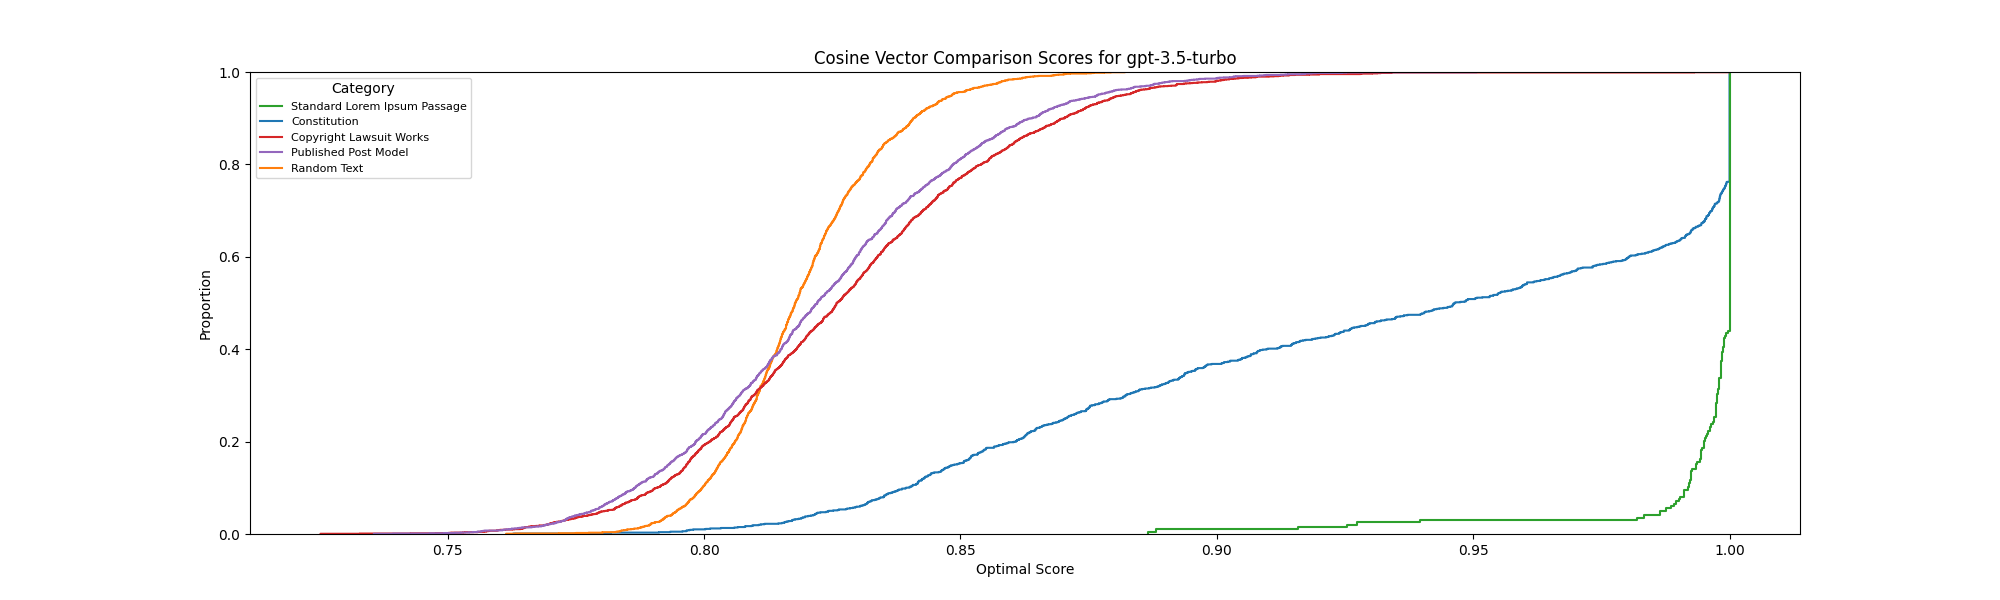
\includegraphics[width=1.0\textwidth]{cosine-ecdf-plot-gpt-3.5-turbo.png}  \\  
% 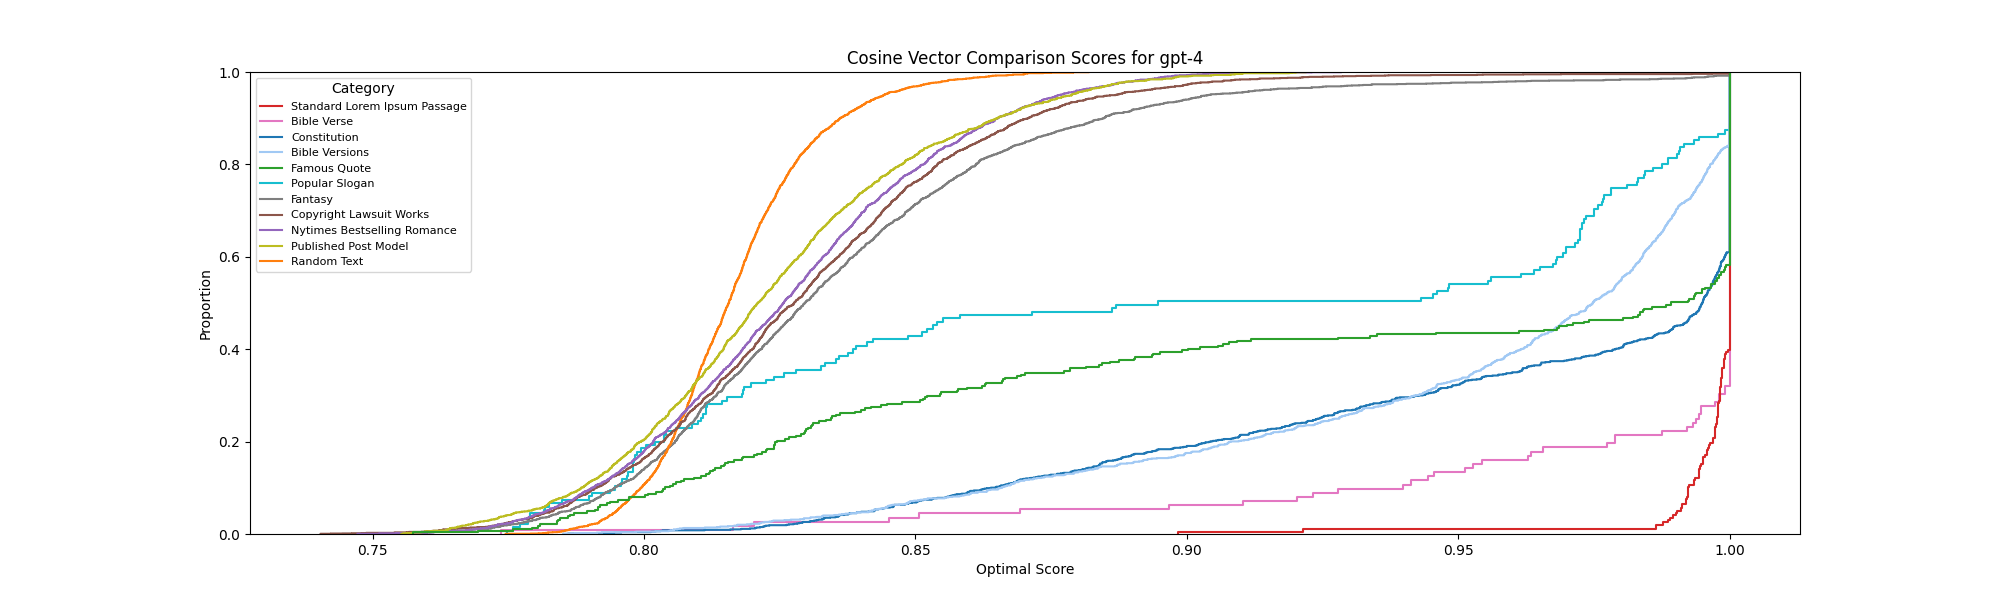
\includegraphics[width=1.0\textwidth]{cosine-ecdf-plot-gpt-4.png}  \\ 
% 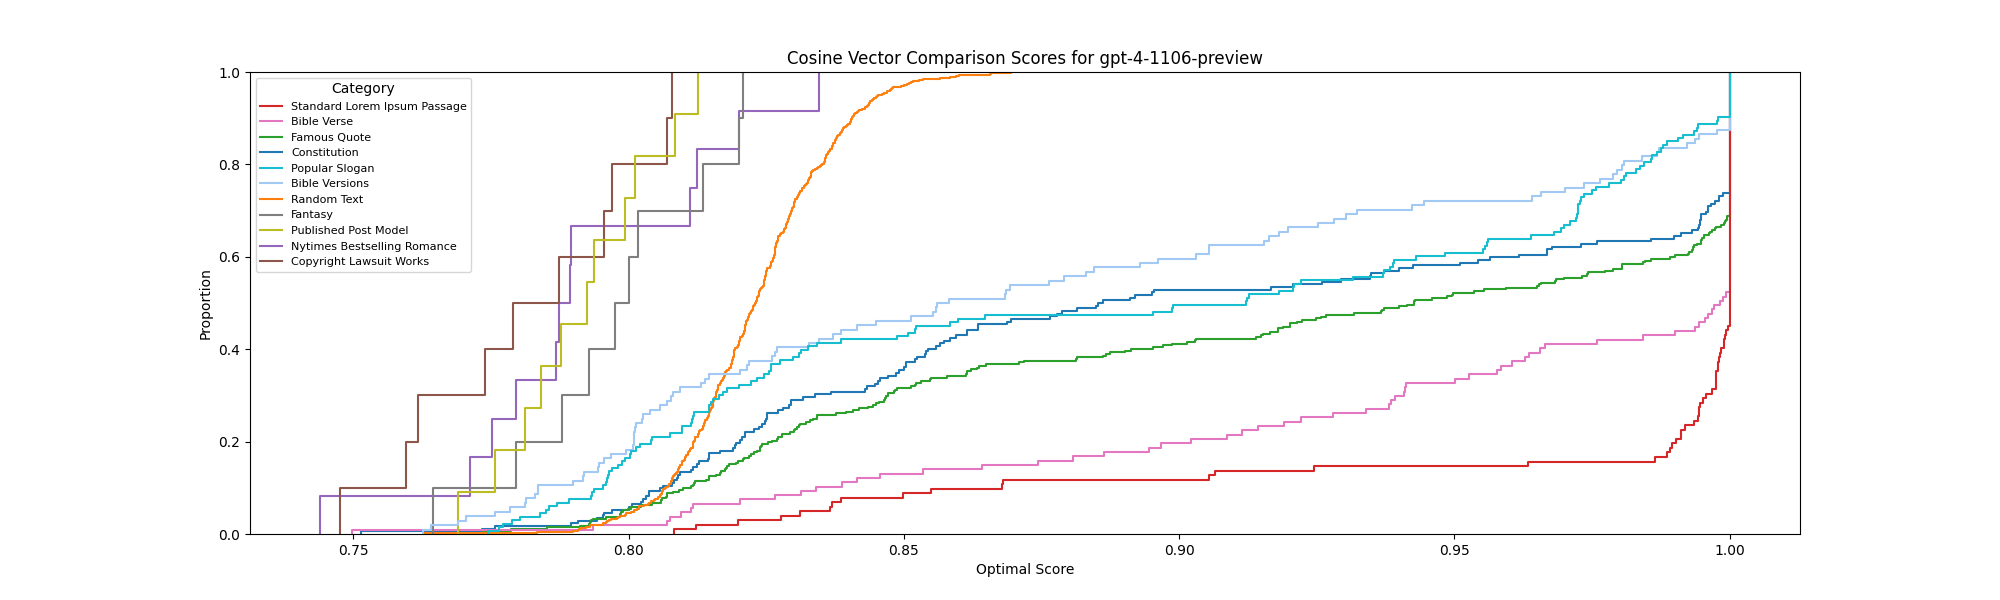
\includegraphics[width=1.0\textwidth]{cosine-ecdf-plot-gpt-4-1106-preview.png}  \\ 
% \end{tabular} 
% \caption{Cosine Similarity ECDF Plot for All Categories} 
% \label{tab:images} 
% \end{table} 

\begin{table}[ht] 
\centering 
\begin{tabular}{ccc} 
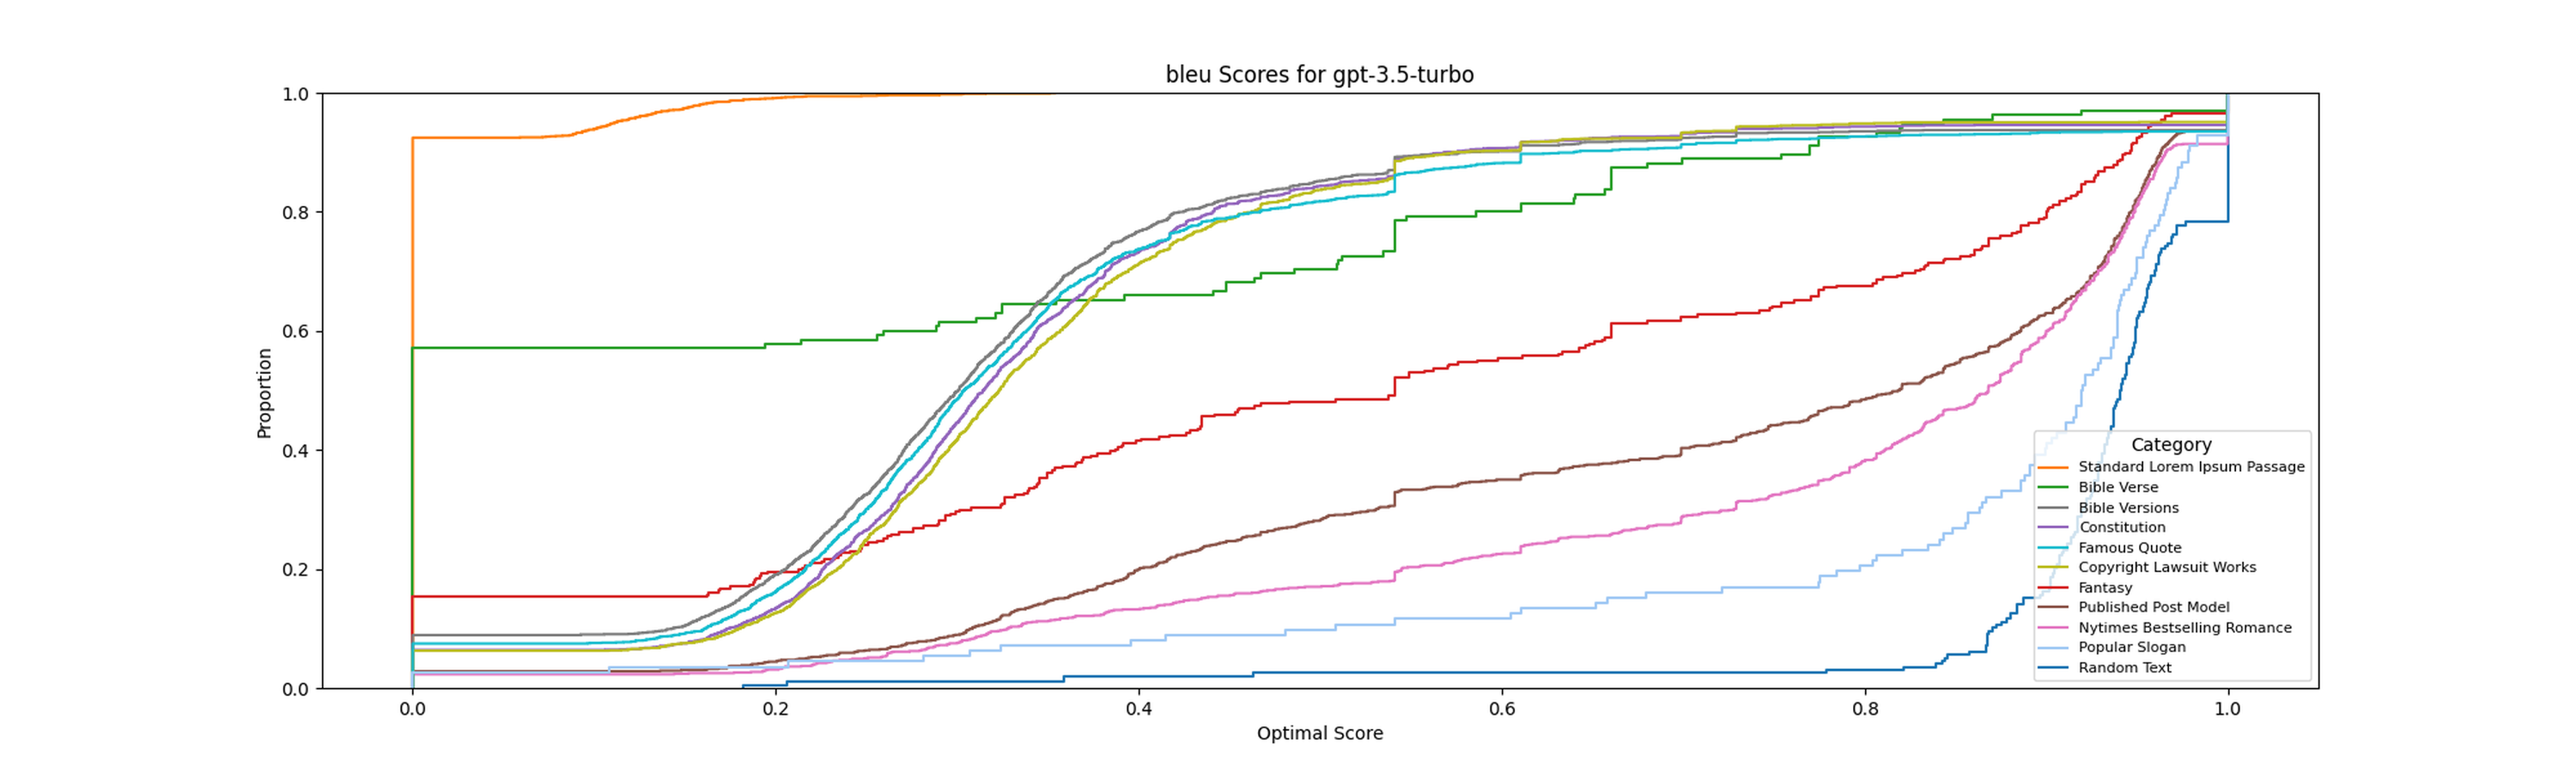
\includegraphics[width=1.0\textwidth]{plots/bleu-ecdf-plot-gpt-3.5-turbo.png}  \\  
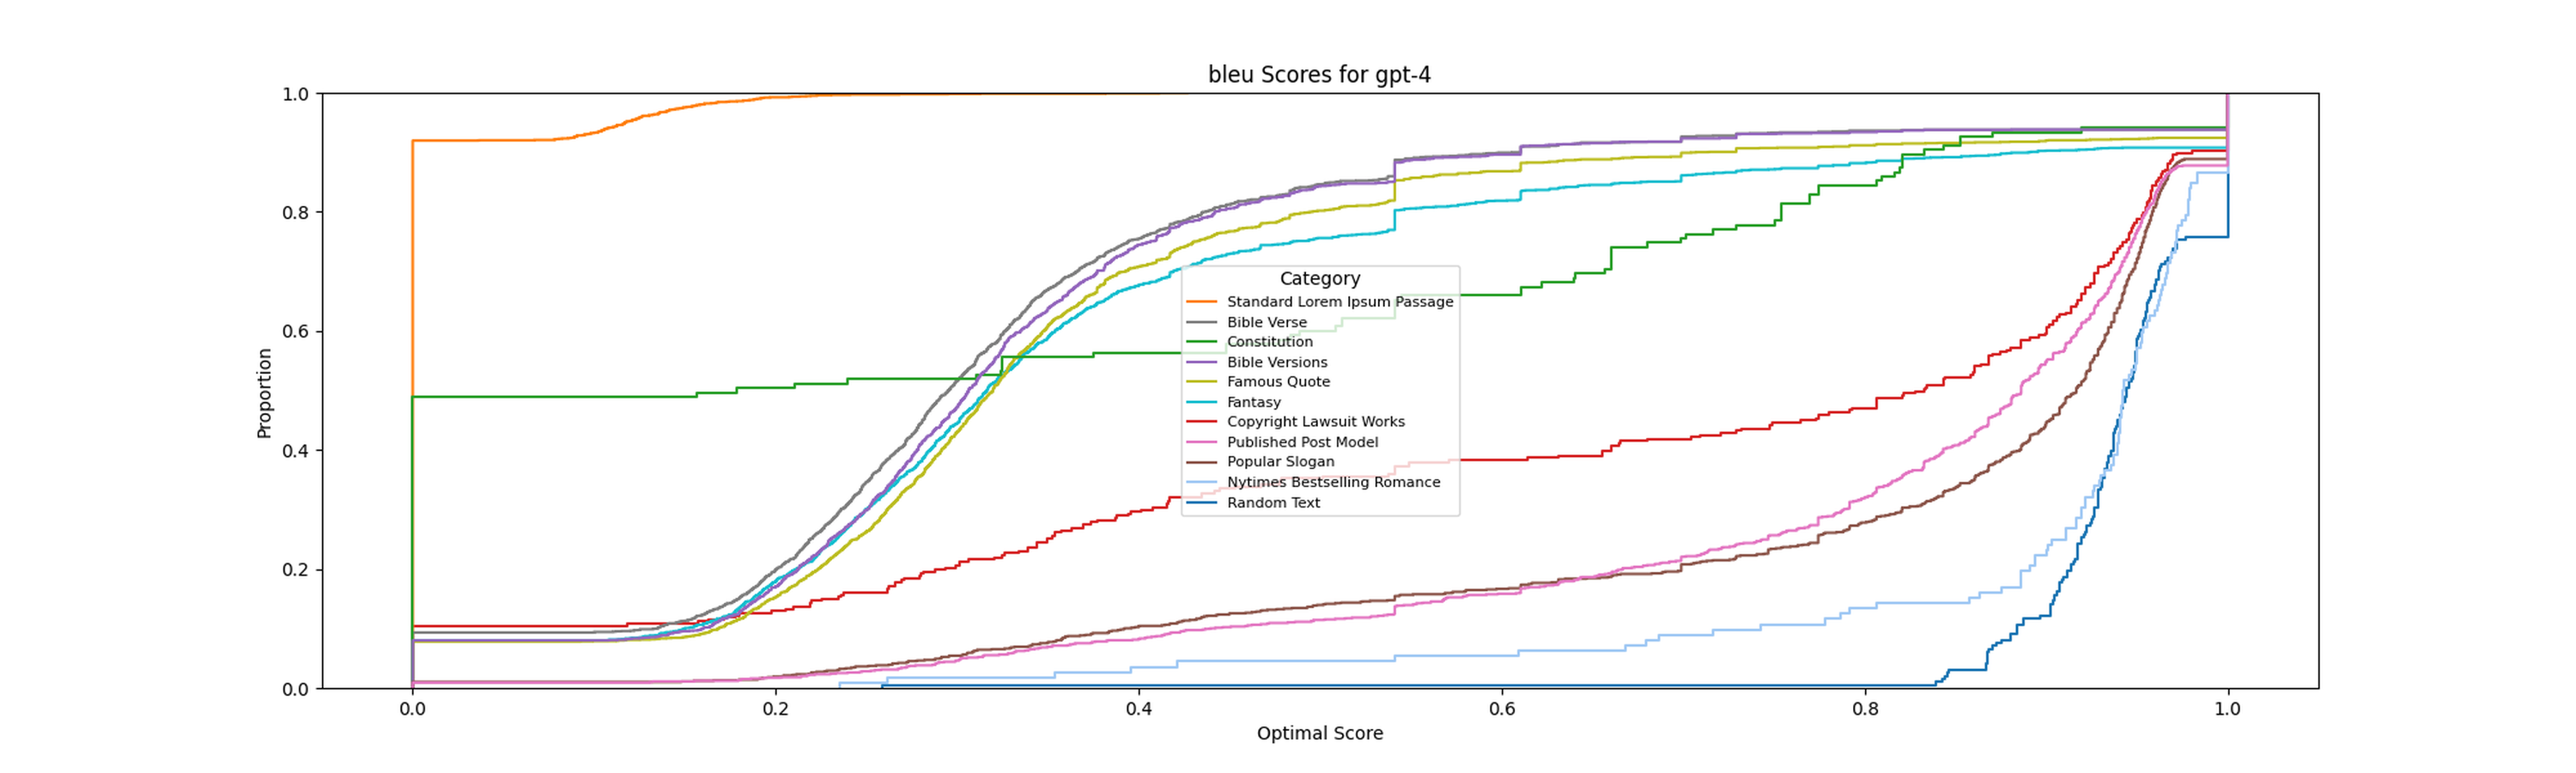
\includegraphics[width=1.0\textwidth]{plots/bleu-ecdf-plot-gpt-4.png}  \\ 
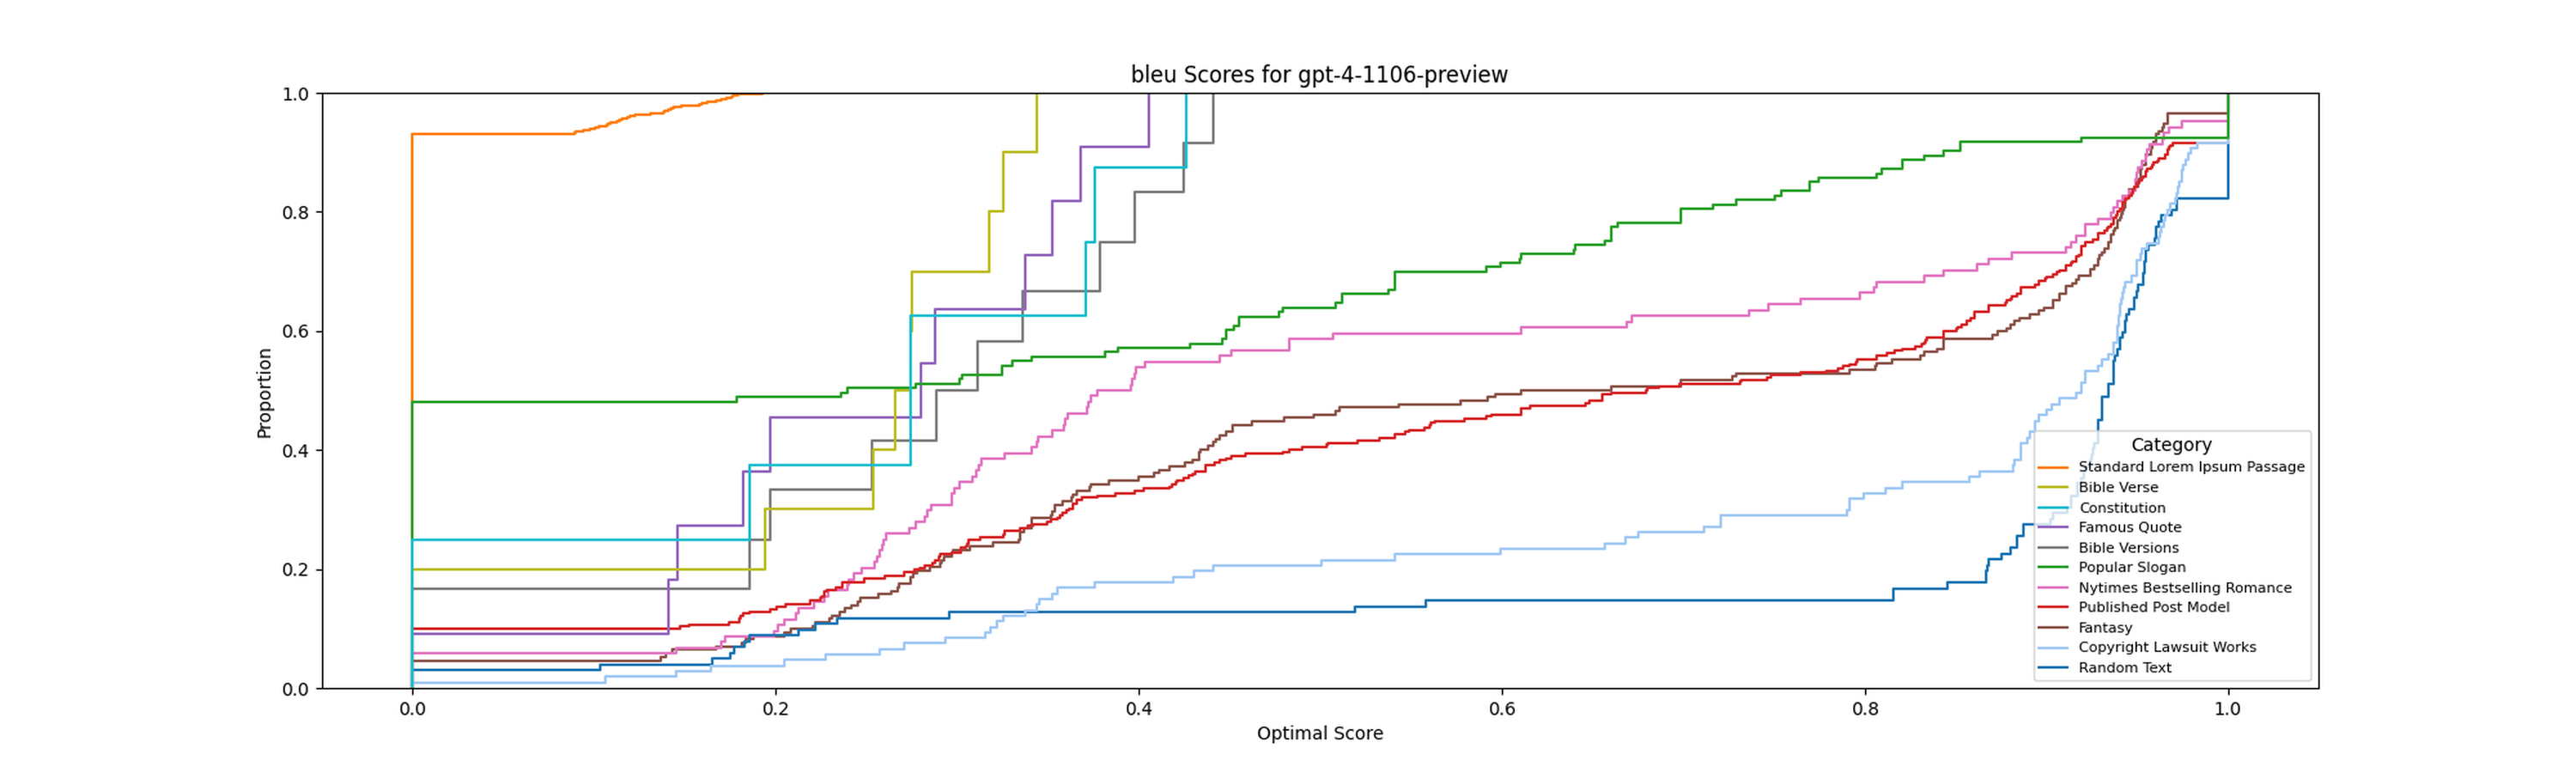
\includegraphics[width=1.0\textwidth]{plots/bleu-ecdf-plot-gpt-4-1106-preview.png}  \\ 
\end{tabular} 
\caption{BLEU Similarity ECDF Plot for All Categories} 
\label{tab:images} 
\end{table}

\begin{table}[htbp]
    \centering
    \caption{Empirical CDF Bleu Scores per Model}
    \begin{tabular}{lrrr}
    \toprule
    Category & gpt-3.5-turbo & gpt-4-1106-preview & gpt-4 \\
    \midrule
    Standard Lorem Ipsum Passage & 1.000000 & 1.000000 & 1.000000 \\
    Random Text & 0.000000 & 0.000000 & 0.000000 \\
    Popular Slogan & 0.263901 & 0.389707 & 0.351767 \\
    Famous Quote & 0.563285 & 0.727591 & 0.688487 \\
    Published Post Model & 0.375558 & 0.287299 & 0.362750 \\
    Constitution & 0.753529 & 0.732690 & 0.860585 \\
    Bible Versions & 0.818209 & 0.629382 & 0.851589 \\
    Nytimes Bestselling Romance & 0.358871 & 0.314567 & 0.350969 \\
    Copyright Lawsuit Works & 0.381860 & 0.262597 & 0.388533 \\
    Fantasy & 0.377908 & 0.278820 & 0.407453 \\
    Bible Verse & 0.899282 & 0.932198 & 0.954506 \\
    \bottomrule
    \end{tabular}
    \caption{TODO: sort by score}
\end{table}

% \begin{table}[ht] 
% \centering 
% \begin{tabular}{ccc} 
% 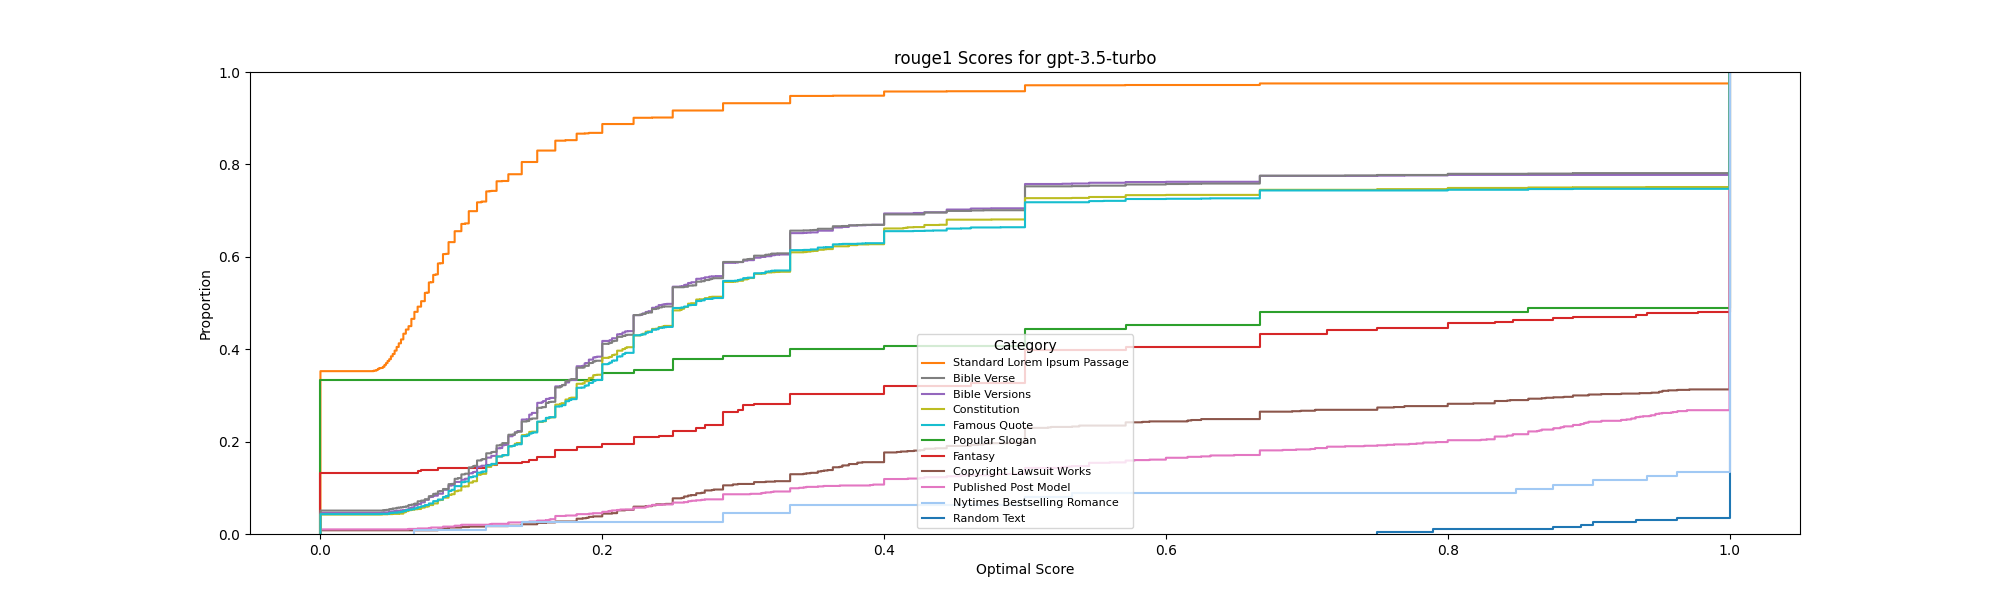
\includegraphics[width=1.0\textwidth]{rouge1-ecdf-plot-gpt-3.5-turbo.png}  \\  
% 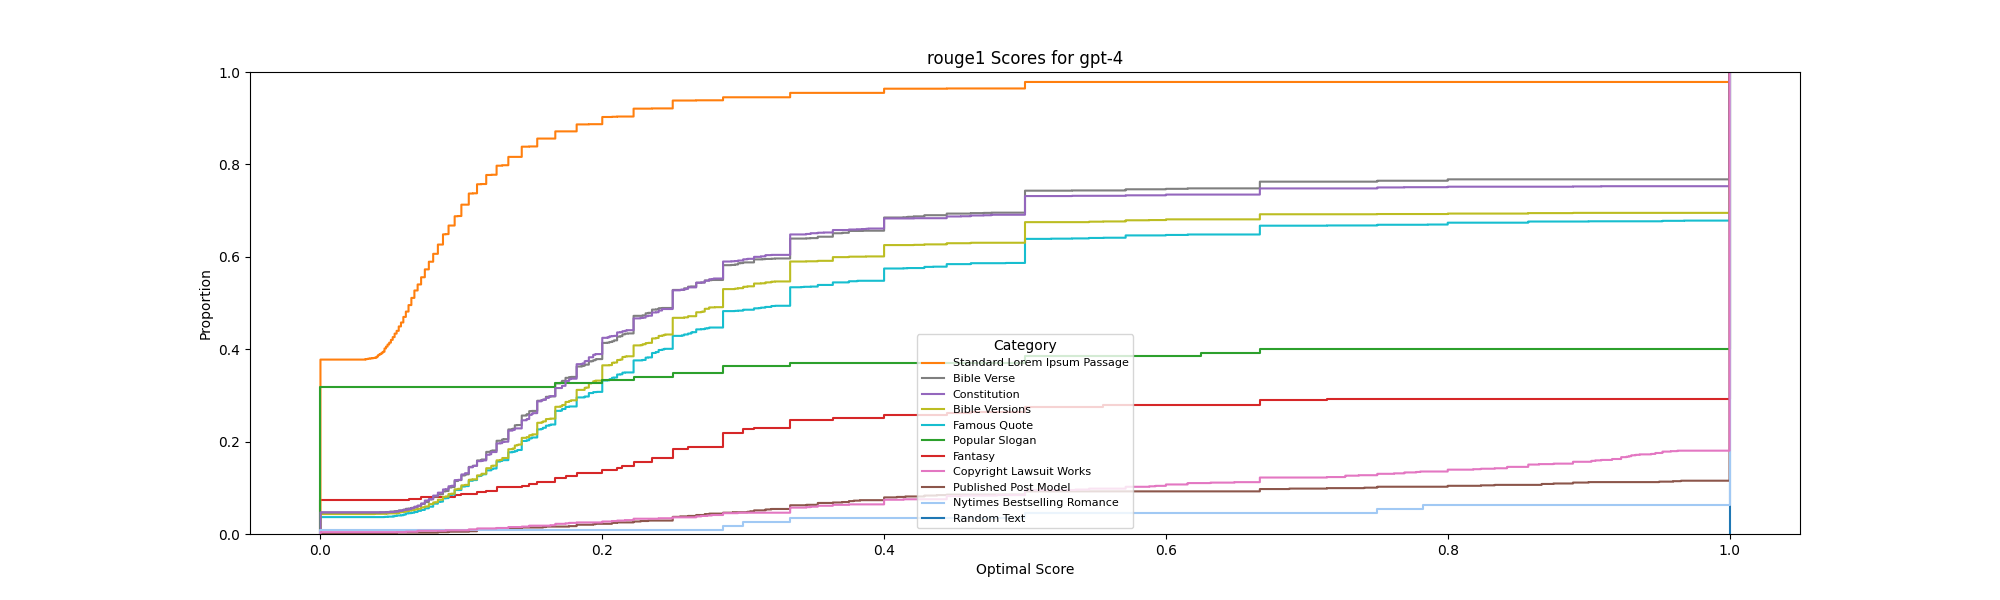
\includegraphics[width=1.0\textwidth]{rouge1-ecdf-plot-gpt-4.png}  \\ 
% 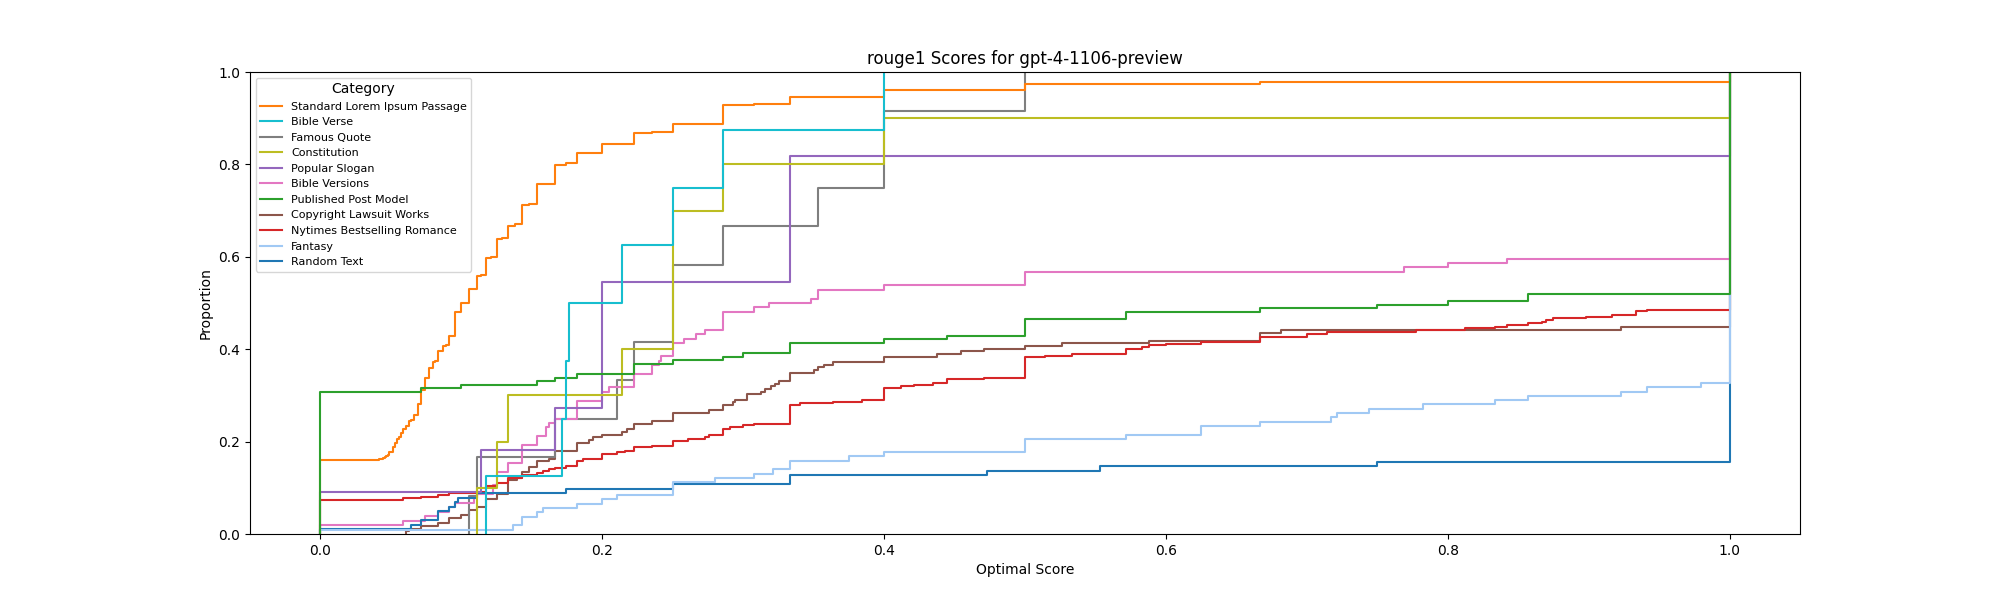
\includegraphics[width=1.0\textwidth]{rouge1-ecdf-plot-gpt-4-1106-preview.png}  \\ 
% \end{tabular} 
% \caption{Rouge1 Similarity ECDF Plot for All Categories} 
% \label{tab:images} 
% \end{table}

% \begin{table}[ht] 
% \centering 
% \begin{tabular}{ccc} 
% 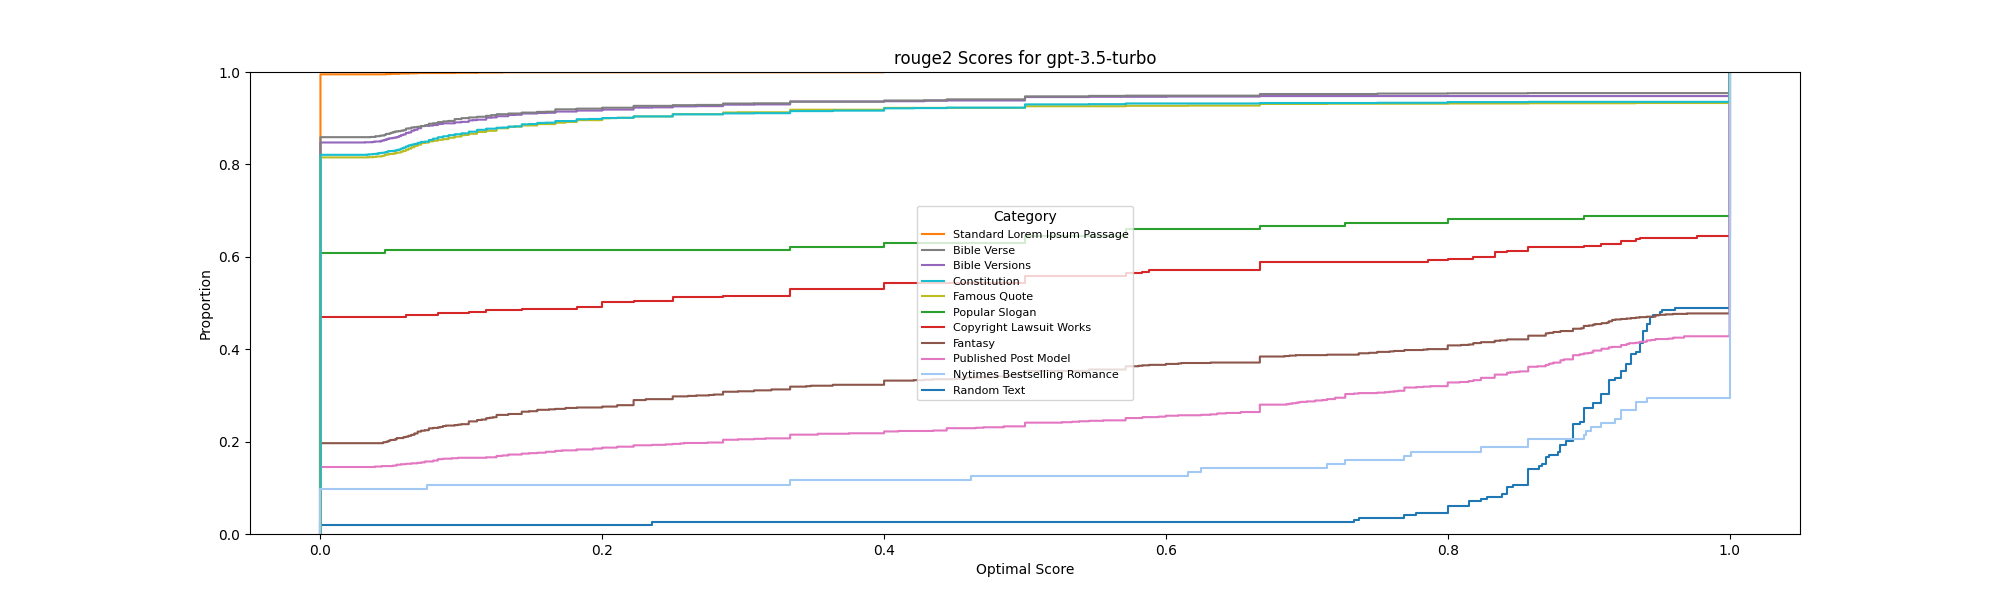
\includegraphics[width=1.0\textwidth]{rouge2-ecdf-plot-gpt-3.5-turbo.png}  \\  
% 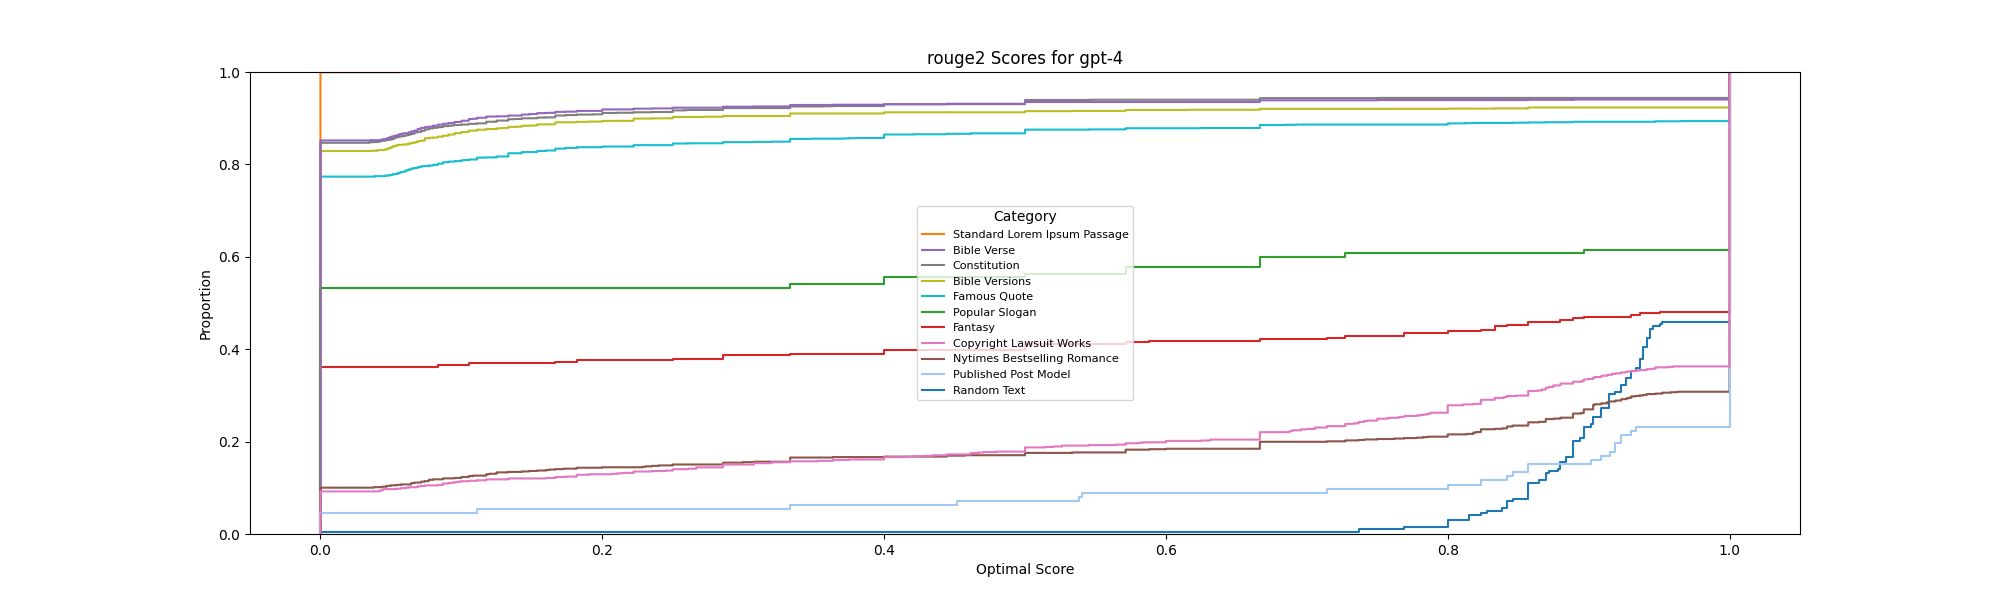
\includegraphics[width=1.0\textwidth]{rouge2-ecdf-plot-gpt-4.png}  \\ 
% 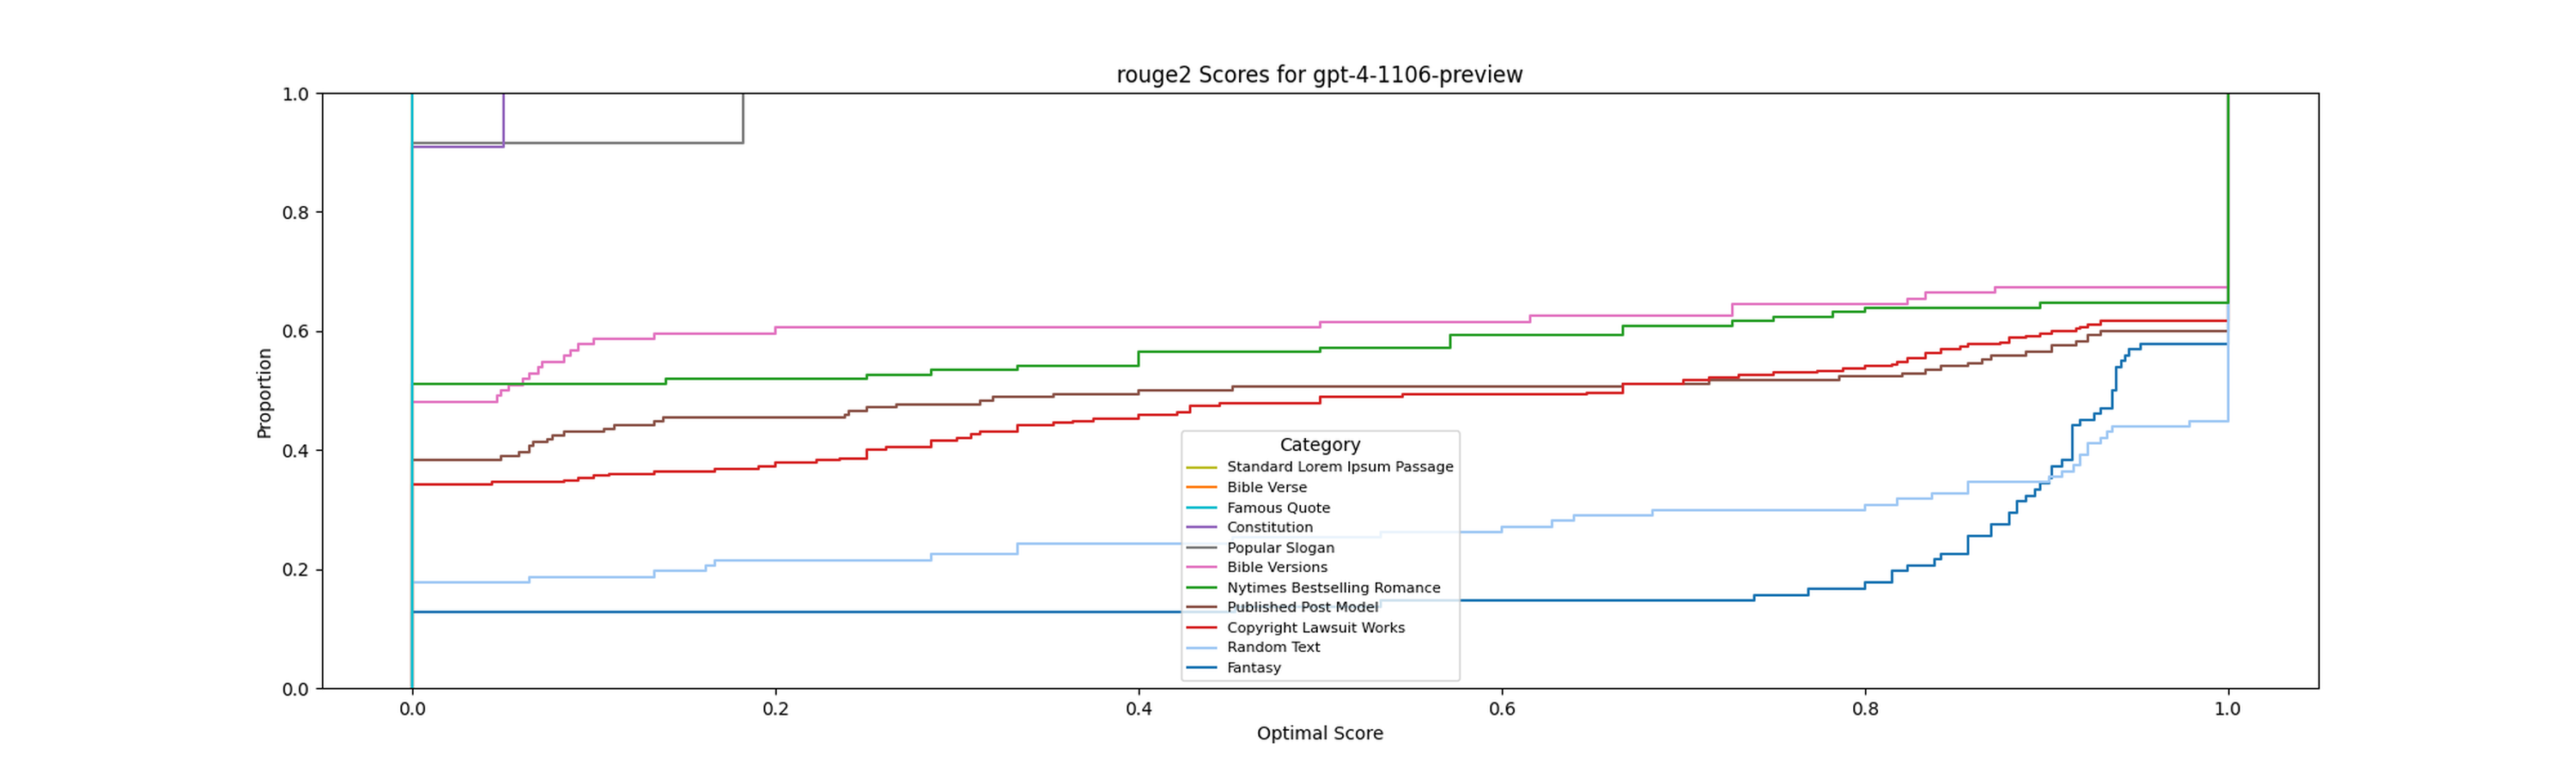
\includegraphics[width=1.0\textwidth]{rouge2-ecdf-plot-gpt-4-1106-preview.png}  \\ 
% \end{tabular} 
% \caption{Rouge2 Similarity ECDF Plot for All Categories} 
% \label{tab:images} 
% \end{table}

% \begin{table}[ht] 
% \centering 
% \begin{tabular}{ccc} 
% 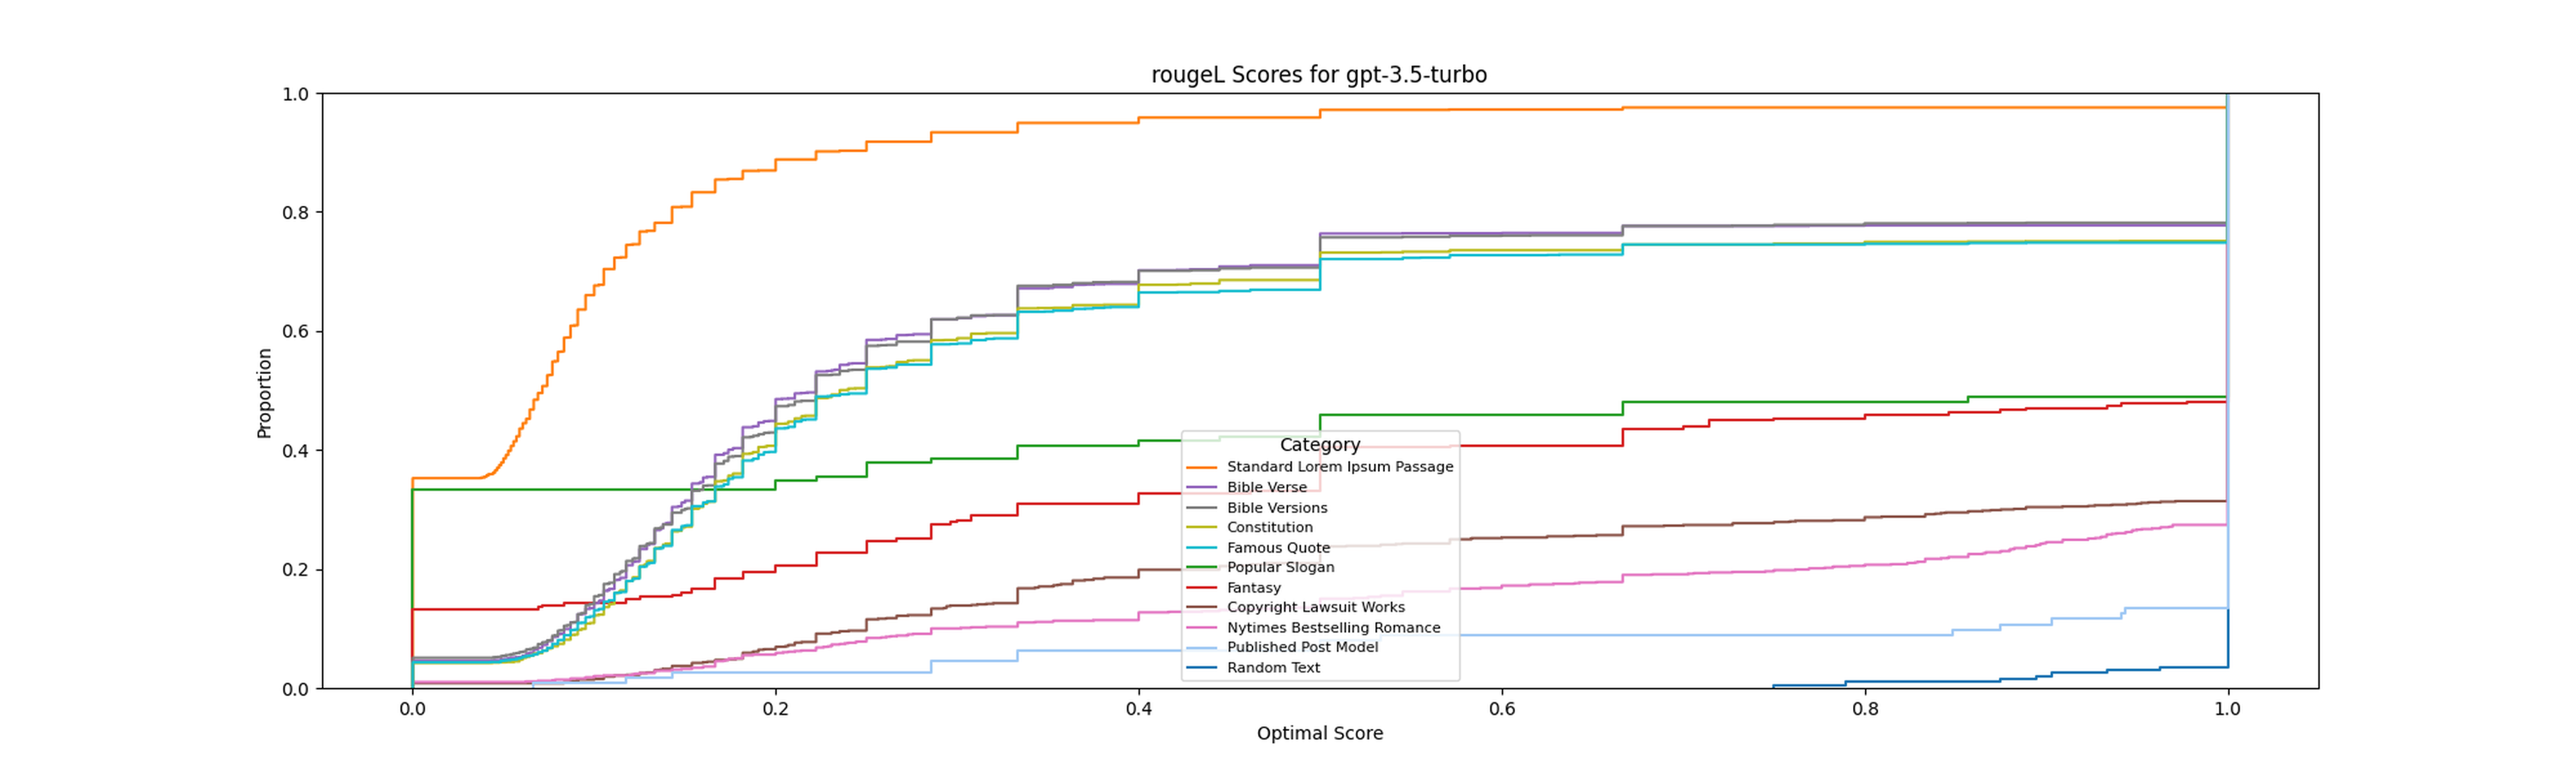
\includegraphics[width=1.0\textwidth]{rougeL-ecdf-plot-gpt-3.5-turbo.png}  \\  
% 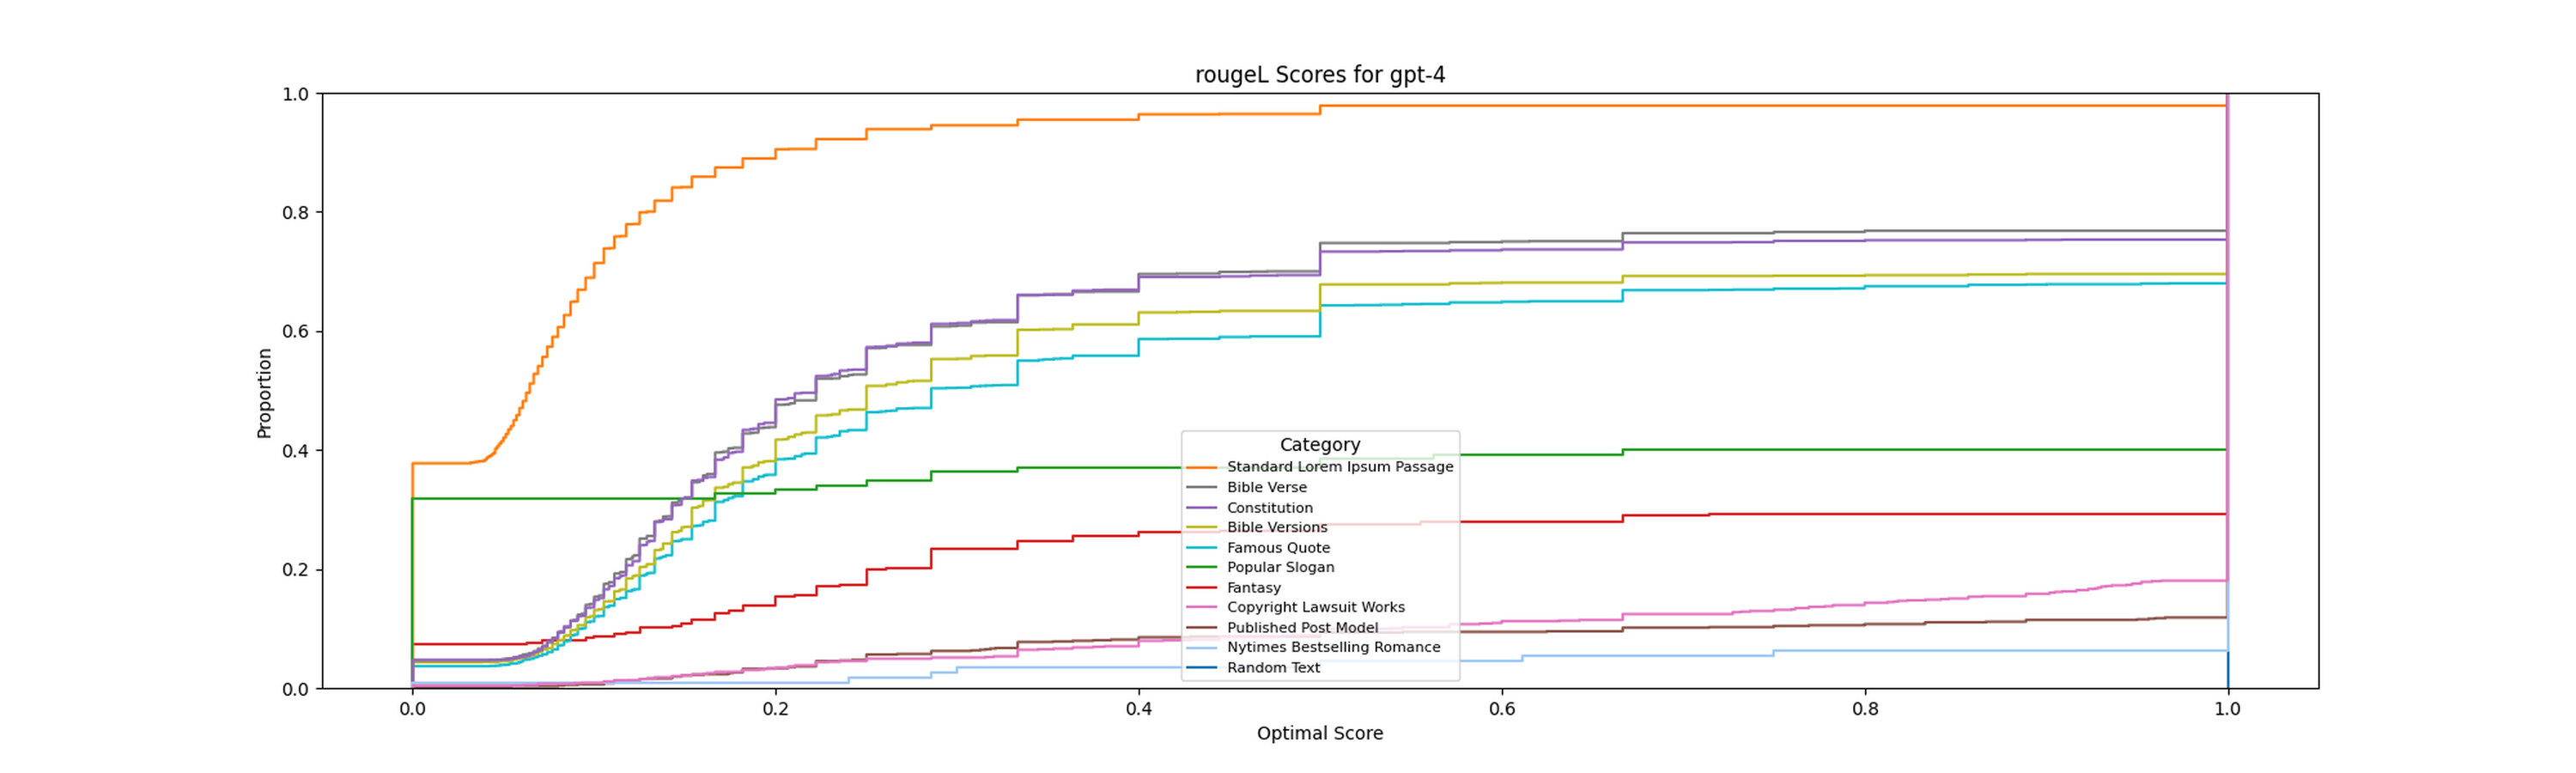
\includegraphics[width=1.0\textwidth]{rougeL-ecdf-plot-gpt-4.png}  \\ 
% 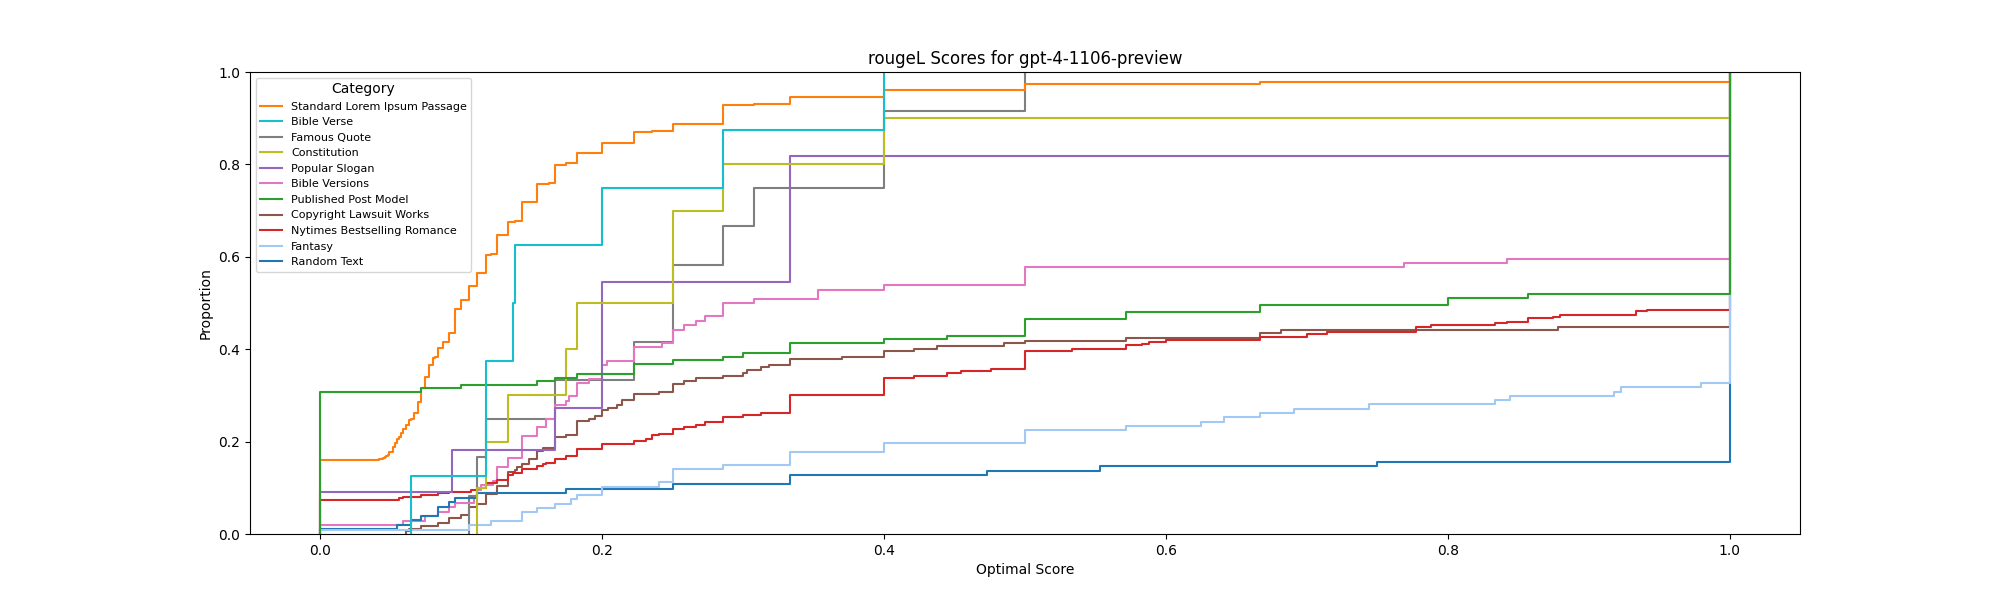
\includegraphics[width=1.0\textwidth]{rougeL-ecdf-plot-gpt-4-1106-preview.png}  \\ 
% \end{tabular} 
% \caption{RougeL Similarity ECDF Plot for All Categories} 
% \label{tab:images} 
% \end{table}

% \begin{table}[ht] 
% \centering 
% \begin{tabular}{ccc} 
% 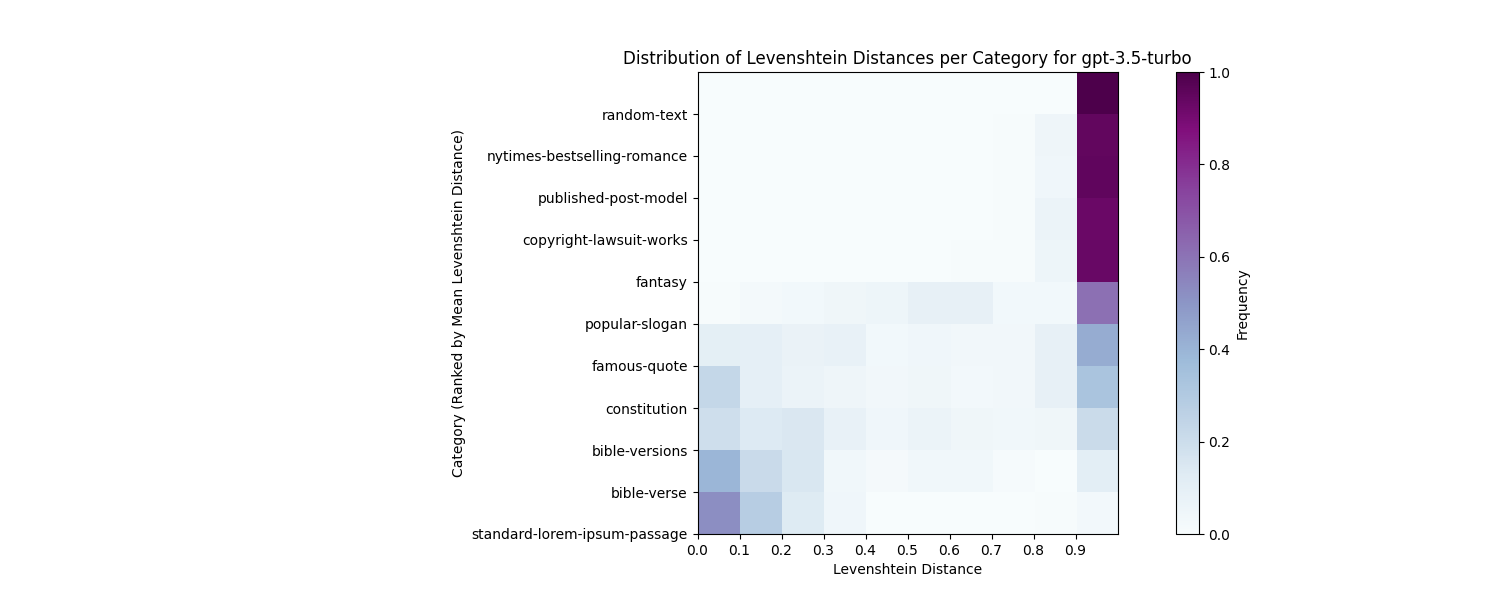
\includegraphics[width=1.0\textwidth]{categories-2d-histogram-gpt-3.5-turbo.png}  \\  
% 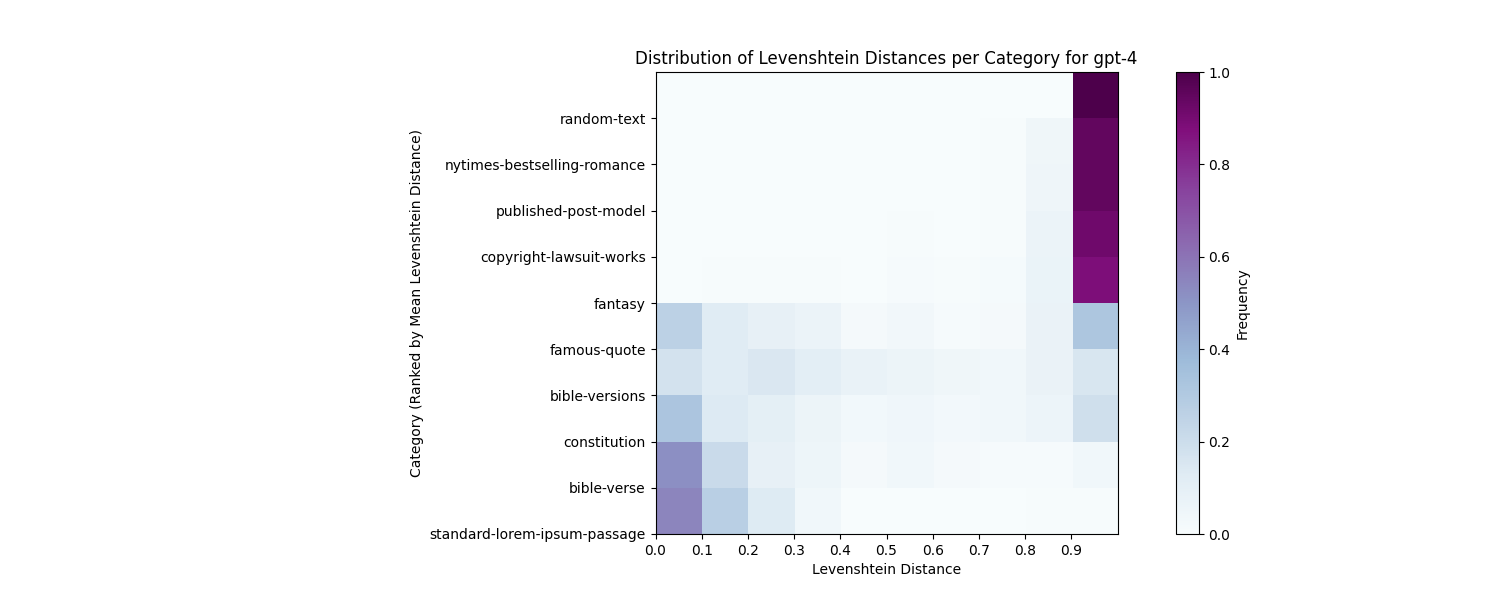
\includegraphics[width=1.0\textwidth]{categories-2d-histogram-gpt-4.png}  \\ 
% 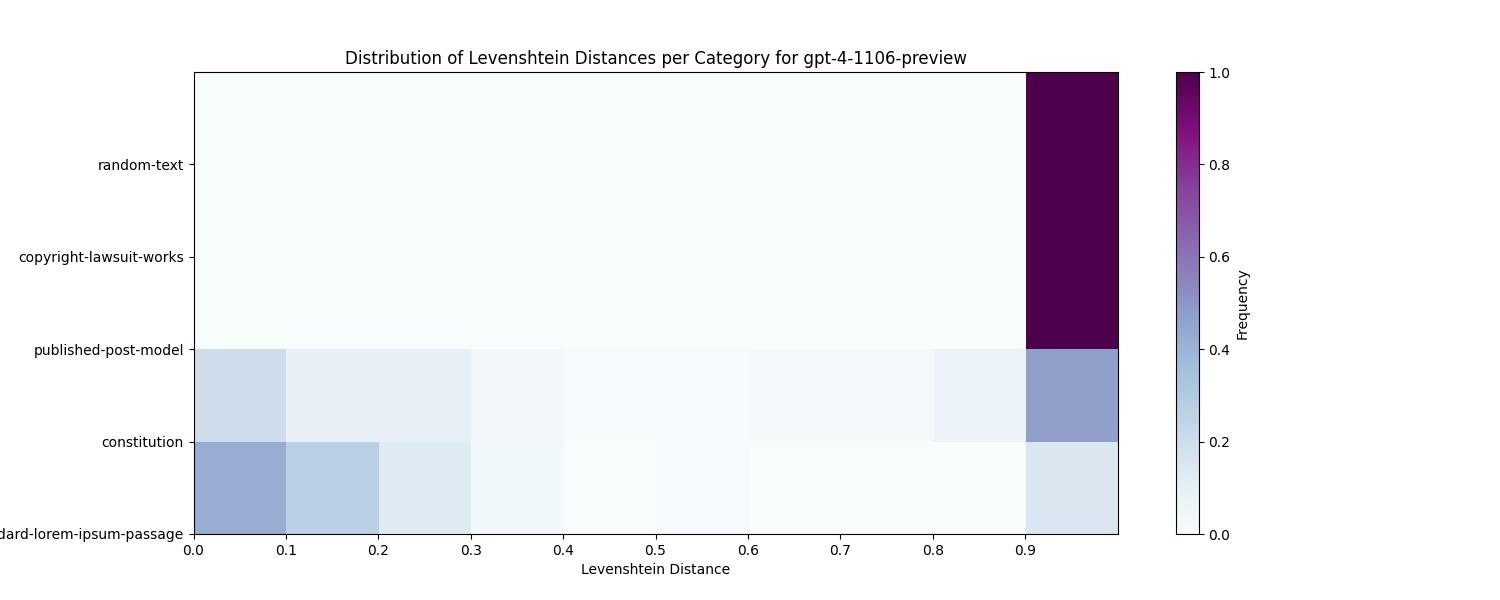
\includegraphics[width=1.0\textwidth]{categories-2d-histogram-gpt-4-1106-preview.png}  \\ 
% \end{tabular} 
% \caption{Levenshtein Distance Distributions per Category} 
% \label{tab:images} 
% \end{table} 



Results were produced on each model through each form of text. The most valuable results are shown through bleu measurements, as visualized through an ECDF graph, table of scores, and number line values. Quantitatively, all scores under the curve were normalized to values between 0 and 1, with Random text as the lower limit and Standard Lorem Ipusm Passage as the upper limit.  

Through each model, non copyrighted works performed better, more accurately quoted, than copyrighted works. Overall categories which produced good results include, Bible versions, Bible verses, Famous Quotes, Popular Slogans, and the Constitution. These are all non copyrighted works which are easily found through many sources online. On the other hand, categories which produced bad results were Fantasy, NY Times Bestselling Romance, and Suing GPT Works, all of which contain copyrighted materials. Further published most model works and copyrighted novels, such as NY Times Bestselling Romance and Fantasy, perform very similarly simply based on common use of language. Specifically, gpt-3.5 scores for published post model is 0.375558 compared to fantasy which is 0.377908. In theory, published post model would perform much worse, yet because of commonality in language, the scores have less variability, and give a lower limit bound of the results. 

As data was generated on three gpt models, gpt-3.5-turbo, gpt-4, and gpt-4-1106 preview, it is important to note the differences between each. In general, gpt-4 scores were slightly better than gpt-3.5, with scores for bible versions of 0.851589 and 0.818209 respectively. Although gpt-4 preview scores were scattered, it is important to note that almost the entirety of results with this model produced the inability to complete the quotes, as stated previously in the prompting section. All of the visualization includes all real responses, that is, those that did not return with a concern over copyright. So these results are not wholly comparable to gpt 3.5 and 4 results due to a smaller amount of quality data. 














\section{Discussion (rough draft)}
\label{sec:discussion}
[Fact check all of this]

Start with a discussion of Jorge Luis Borges's short story, "Pierre Menard, Author of the Quixote," in which the eponymous author Pierre Menard sets off to reproduce to the exact letter the entirety of Miguel Cervantes's famous novel \emph{Don Quixote}. Quote from it about how [CITE] the author-narrator visits Spain, adopts a particular lifestyle in the hopes that method acting like Cervantes will reproduce the exact text--and it does. The fictional critics of Pierre Menard's new text discuss how much richer it is in meaning, despite the fact that they are exactly the same words. What might we take from this critique of quotation to answer questions about copyright infringement and text-reproduction equivalence? Versus SMAUC optimization where GenAI can approximate the same meanings using a probabilistic approach. [Idea: look into the context in which "meaning" is measured, as it may be a question of scope of reading context rather than a sole focus on the text itself, which is what our project does with cosine similarity, whether with embeddings or exact character/token replacement.]

In analyzing the ability of GenAI to quote sources from its training data, our project indexes a set of related fields beyond computer science, including attribution studies, the history of material texts, and library science. Accordingly, we conducted the experiments in our study with the goal not only of identifying objective criteria to measure GenAI’s ability to reproduce quotes verbatim but also to test the cultural and legal definitions of quotation itself. The urgency of these questions at the time of writing in 2024 are readily apparent. Watershed legal cases over copyright have already started taking form between high-status institutions including \emph{The New York Times}, OpenAI, Microsoft, and Google [CITE]. 

However, it is important to note that the practice of quotation and citation as well as the legal definition of copyright have been in flux essentially from their very invention. The practice of quotation extends back to classical antiquity, where ancient teachers and their students would memorize popular aphorisms to pass down wisdom and cultivate arguments for rhetorical debate. [CITE: Find example of Plato, or Homer, or early Christian theologians, provide example.] This practice continued for centuries among oral and manuscript cultures in the Western world until the print revolution in medieval Europe in the 15th century [CITE: look into \emph{The Printing Revolution in Early Modern Europe}]. At that time, systems of reference evolved to better organize the vast stores of texts that started to proliferate among libraries, and as a result, it was in this era that the modern practice of textual citation began to develop to keep track not only of quotes but also their textual provenance [Fact check here, look at library science to see about organizational systems for library management, see about attribution studies and citaitons]. 

Academic citation in its early forms from the 16th century onward was an imperfect art because the culture of crediting authors for their ideas and work was in a nascent state. Indeed, religious tradition credited ideas in the first instance not to authors but to God; from the Christian God as Word to Allah’s first action to create a pen as according to Islamic tradition, the practice of attributing quotations to original sources was always already complicated, especially in writing. [Cite Islamic scholars on the significance of Allah’s first act to create a pen; cite a well-known Christian theologian (Thomas Aquinas?) about the symbolism of the Christian God as Word—perhaps cite Quine on \emph{Word and Object})

In the 19th and 20th centuries, with the rise of industrialization across the globe as well as concomitant rise of juridical institutions to protect property rights, including intellectual property rights, academic citation transitioned from a marginalized intellectual tradition to a social ethic. Colleges and universities established standards of citational practice as well as ethical guidelines governing what counted as plagiarism and how to discipline instances of it. Academic journals and print publishers quietly became the arbiters of intellectual thought not only as a scholarly activity but indeed as a culture industry in which index rankings, impact factors, and reference counts became social currency. [Find references for critical analyses of academic scholarship publication] [Discuss the founding and rise of organizations such as the Modern Language Association and the American Psychological Association as well as their style guides, etc., Chicago as oldest in 1891]

While citational practice in the contemporary era has the veneer of professional excellence and intellectual objectivity, there have always been cracks in its foundation. In the past decade, for instance, the “replication crisis” has plagued academic science and resulted in a uneven approach to article retractions in which faulty original research has been exposed but not the extent of its spread via citations in other papers. Most recently, high profile figures in the academic world have been confronted with career-altering accusations of plagiarism. [CITE: president of Harvard who recently stepped down; famous Stanford professor whose name I can’t remember; others, etc.] With such dire consequences attached to academic honesty in which proper attribution is a professional and ethical imperative, it is striking that our study has revealed the computational pitfalls of generating quotes using probabilistic transformer models. 

What will the standards for quotation and intellectual property look like in the future where text-generation technologies have proliferated in every culture across the globe? 

Discussion of the threshold for quote veracity, which seems to trouble questions of semantic embedding similarities (cosine approach) and information theory approaches (Levenschetin (sp?) approach) to measuring ability to quote.

Discussion of cryptography and spoofing text using homograph attacks to produce text that looks like an exact quote but uses different glyphs at a subliminal level.

Discussion of the challenges that will face copyright law to articulate policies and procedures that govern text generation while also adhering to a robust and informed sense of the technology’s underlying methods. Discussion of what intellectual property rights will need to be discarded now that Pandora’s Box has been opened, but also a historical argument for how this has always been happening and how we might extrapolate from this iteration of the process. Discussion about open access to information (Aaron Schwartz) and how the destabilization of intellectual property rights does not necessarily destabilizes the ideas that they were created to protect.
[Find what to cut that is beyond scope of project]


\section{Future Work}
\label{sec:future-work}

explore impact of punctuation, stage direction, LaTeX commands, etc. on reproduction quality

\section{Conclusion}
\label{sec:conclusion}


\bibliographystyle{hunsrtnat}
\bibliography{references}

\section{Appendix}

Chat Completion Example, Published Post Model and Novel Directory:
    \begin{verbatim}
    "Finish the rest of the paragraph. It is from {title} by {author}." 
    \end{verbatim}
    
    
Chat Completion Example, Constitution Directory:
    \begin{verbatim}
    "Finish the rest of the paragraph. It is from {title} of the US Constitution."
    \end{verbatim}
    

Chat Completion Example, Short Sentences Directory:
    \begin{verbatim}
    "Finish the rest of the sentence. It is a {sentence-type}." 
    \end{verbatim}
    
    
Chat Completion Example, Bible Versions Directory:
    \begin{verbatim}
    "Finish the rest of the paragraph. It is from the {bible-name}."
    \end{verbatim}


Chat Completion Example, Standard Lorem Ipsum:
    \begin{verbatim}
    "Finish the rest of the paragraph. It is from the {standard-lorem-ipsum}"
    \end{verbatim}


Chat Completion Example, Random Text:
    \begin{verbatim}
    "Finish the rest of the paragraph. It is {random-text}"
    \end{verbatim}



\subsection{Alternative Metrics}

\subsubsection{Levenshtein Distance}

Histograms

BIBLE VERSIONS 



SUING COPYRIGHTED WORKS 



FAMOUS SLOGANS



2D Histogram






\subsubsection{Cosine Embedding Vectors}
Sentence Length Line Graphs




ECDF


Levenshetin vs Cosine Scatter Plot




GRAPH/TABLE NOTES

MOST IMPORTANT: 
1) We have put these at the beginning of the RESULTS section, starting on line 285-ECDF plots across text types per model (pg6-10), 2D histograms that compare across text types per model (pg15). These are the most important forms of visualization because they allow you to easily see the difference across categories, and highlights how stark the difference is between each category. 

2)To show the difference in performance between models using Levenshtein, we have chosen the constitution 2D histograms(pg.52). Since this is not a copyrighted work, it does a good job of showing how well each model quotes in comparison. 

3) To show how well things that have been seen a lot can be quoted, the bible verses histograms do a good job of representing that(pg.27).

4) To show how bad and how unfounded lawsuits are, the Copyrighted Works and Published Post Model histograms and scatterplots represent this due to their results and similarity (pgs. 58, 60and pgs ). 

5) ECDF Cosine Scores table per model, which gives the numeric value of the distance under the curve for each text category, at the beginning of the Appendix (lines 743-851 and pgs 17-19). 

SUMMARY OF GRAPHS/TABLES

For each text type, we have Levenshtein Histograms, 4 types of scatter plots (Lev v Cosine, Bleu v Cosine, Rouge1 v Cosine, Rouge2 v Cosine, RougeL v Cosine), all each per model (3.5,4.0, 4.0 preview)

For text types that have more varied distribution of data, we have 2D histograms per model. 

We have 2D histograms that compare across text types per model.
We have ECDF plots that compare across text types per model. 

For tables, we have a table that shows average length in tokens of prompted previx and actual suffix, as well as a table of the average length for the predicted suffix per model. 

We also have an ECDF Cosine Scores table per model, which gives the numeric value of the distance under the curve for each text category. These are very important and are at the beginning of the Appendix (lines 743-851), shown on pages 17-19. 




%\setlength\parindent{50pt}
%    \setlength{\fboxsep}{10pt}\fbox{%
%    \begin{minipage}{30em}
%Original: \texttt{\textcolor{teal}{Quote quote quote quote quote quote}}
%    \newline Completion:  \texttt{\highLight{teal}{Quote quote %quote}\highLight{red}{misquote misquote misquote}} 
%    \end{minipage}
%  }






\subsection{Text Sources}

\textbf{Bible Versions}

Amplified Bible

Christian Standard Bible

English Standard Bible

King James Bible

New Living Translation Bible


\textbf{NY-Times Bestselling Romance}

D'Vaughn and Kris Plan a Wedding by Chencia Higgins

Electric Idol by Katee Robert

Fire Season by KD Casey

Ocean Echo by Everina Maxwell

Something Fabulous by Alexis Hall

Tanked by Mia Hopkins

Thank you for Listening by Julia Whelan

The Dead Romantics by Ashley Poston

The Very Secret Society of Witches by Sangu Mandanna

You Made a Fool of Death with Your Beauty by Akwaeke Emexi

\textbf{Fantasy}

American Gods by Neil Gaiman

Circe by Madeline 

Game of Thrones by George Martin

Harry Potter by JK Rowling

Lord of the Rings by JRR Tolkien

Six of Crows by Leigh Bardugo

The Blade Itself by Joe Abercrombie

The Name of the Wind by Patrick Rothfuss

The Nigh Circus by Erin Morgenstern

The Poppy War by RF Kuang

\textbf{Popular Slogans}

Popular Slogans and Famous Ad Jingles from Sports Feel Good Stories
11 Classic Examples Of Exceptional Jingle and Slogan Writing from Search Engine Journal


\textbf{Famous Quotes}

Quotes.txt from Rob McGuire (Robatron on GitHub)


\textbf{Bible Verses}

The Most Popular Verses of the Bible from Bible Lyfe 
Popular Bible Verses from King James Bible Online
25 Famous Bible Verses from SeedTime
50 Most Popular Bible Verses from Bible Study Tools


\subsection{Tables}



\begin{table}[htbp]
    \centering
    \caption{Average Length in Tokens}
    \begin{tabular}{lcc}
        \toprule
        Model and Dataset & Prompted Prefix & Actual Suffix\\
        \midrule
        \multicolumn{4}{l}{\textbf{GPT 3.5 Turbo}} \\
        \midrule
        Bible Verses & 9.4 & 19.6 \\
        Constitution & 9.8 & 18.9 \\
        Copyright Lawsuit Works & 9.8 & 19.7 \\
        Famous Quotes & 5.7 & 10.5 \\
        Popular Slogans & 2.5 & 4.3 \\
        Published Post Model & 9.9 & 20.0 \\
        Random Text & 9.9 & 18.8 \\
        Standard Lorem Ipsum Passage & 9.8 & 20.3 \\

        \midrule
        \multicolumn{4}{l}{\textbf{GPT 4}} \\
        \midrule
        Bible Verses & 9.4 & 22.0 \\
        Constitution & 9.8 & 20.3 \\
        Copyright Lawsuit Works & 9.8 & 20.0 \\
        Famous Quotes & 5.7 & 12.3 \\
        Popular Slogans & 2.5 & 4.6 \\
        Published Post Model & 9.9 & 20.0 \\
        Random Text & 9.8 & 20.0 \\
        Standard Lorem Ipsum Passage & 9.8 & 20.3 \\

        \midrule
        \multicolumn{4}{l}{\textbf{GPT 4 Preview}} \\
        \midrule
        Bible Verses & 9.7 & 22.7 \\
        Constitution & 10.0 & 19.2 \\
        Copyright Lawsuit Works & 7.7 & 23.4 \\
        Famous Quotes & 5.7 & 14.2 \\
        Popular Slogans & 2.6 & 5.0 \\
        Published Post Model & 8.3 & 21.0 \\
        Random Text & 9.1 & 20.2 \\
        Standard Lorem Ipsum Passage & 10.3 & 20.3 \\

        \bottomrule
    \end{tabular}
    \label{tab:avg_values}
\end{table}


\begin{table}[htbp]
    \centering
    \caption{Average Length in Tokens of Predicted Suffix}
    \begin{tabular}{lccc}
        \toprule
        Model and Dataset & Levenshtein & Optimal Cosine & Bleu / Rouge 1 / Rouge 2 / Rouge L\\
        \midrule
        \multicolumn{4}{l}{\textbf{GPT 3.5 Turbo}} \\
        \midrule
        Bible Verses & 19.5 & 16.8 & 163.3\\
        Constitution & 18.8 & 16.5 & 172.3\\
        Copyright Lawsuit Works & 19.6 & 16.7 & 174.5  \\
        Famous Quotes & 10.5 & 9.0 & 92.5 \\
        Popular Slogans & 4.1 & 3.3 & 34.2  \\
        Published Post Model & 19.8 & 16.2 & 177.1 \\
        Random Text & 18.9 & 6.9 & 195.3 \\
	Standard Lorem Ipsum Passage & 20.3 & 15.2 & 172.7 \\


        \midrule
        \multicolumn{4}{l}{\textbf{GPT 4}} \\
        \midrule
        Bible Verses & 22.0 & 18.7 & 183.2  \\
        Constitution & 19.7 & 17.0 & 179.0 \\
        Copyright Lawsuit Works & 19.7 & 16.5 & 175.0 \\
        Famous Quotes & 12.2 & 10.5 & 107.2  \\
        Popular Slogans & 4.4 & 3.6 & 36.3 \\
        Published Post Model & 19.8 & 16.1 & 177.2 \\
        Random Text & 20.1 & 6.7 & 207.7 \\
        Standard Lorem Ipsum Passage & 20.3 & 15.3 & 172.7 \\


        \midrule
        \multicolumn{4}{l}{\textbf{GPT 4 Preview}} \\
        \midrule
        Bible Verses & 22.6 & 19.8 & 191.3 \\
        Constitution & 18.8 & 20.5 & 174.7  \\
        Copyright Lawsuit Works & 22.2 & 14.3 & 195.6 \\
        Famous Quotes & 14.1 & 13.3 & 125.4 \\
        Popular Slogans & 4.7 & 4.6 & 40.7 \\
        Published Post Model & 20.9 & 11.9 & 195.3 \\
        Random Text & 19.4 & 19.0 & 207.2 \\
        Standard Lorem Ipsum Passage & 20.2 & 17.2 & 176.5 \\


        \bottomrule
    \end{tabular}
    \label{tab:avg_values}
\end{table}




\begin{table}[htbp]
    \centering
    \caption{Empirical CDF Cosine Scores per Model}
    \begin{tabular}{lrrr}
    \toprule
    Category & gpt-3.5-turbo & gpt-4-1106-preview & gpt-4 \\
    \midrule
    Standard Lorem Ipsum Passage & 1.000000 & 1.000000 & 1.000000 \\
    Random Text & 0.000000 & 0.214102 & 0.000000 \\
    Popular Slogan & 0.321436 & 0.578243 & 0.448703 \\
    Famous Quote & 0.440346 & 0.710745 & 0.610041 \\
    Published Post Model & 0.026576  & 0.050908 & 0.038320 \\
    Constitution & 0.640105 & 0.636652 & 0.788686 \\
    Bible Versions & 0.678951 & 0.501751 & 0.755707 \\
    Nytimes Bestselling Romance & 0.036873 & 0.053124 & 0.055115 \\
    Copyright Lawsuit Works & 0.049669 & 0.000000 & 0.073757 \\
    Fantasy & 0.063105 & 0.112152  & 0.106996 \\
    Bible Verse & 0.851441 & 0.886521 & 0.913040 \\
    Gpt Results.Csv & 0.232431 & 0.391601 & 0.209249 \\
    Gibberish Article Results.Csv & 0.060079 & 0.217117 & 0.160623 \\
\bottomrule
\end{tabular}
\end{table}


\begin{table}[htbp]
    \centering
    \caption{Empirical CDF Rouge1 Scores per Model}
    \begin{tabular}{lrrr}
    \toprule
    Category & gpt-3.5-turbo & gpt-4-1106-preview & gpt-4 \\
    \midrule
    Standard Lorem Ipsum Passage & 1.000000 & 1.000000 & 1.000000 \\
    Random Text & 0.000000 & 0.000000 & 0.000000 \\
    Popular Slogan & 0.531683 & 0.580688 & 0.590253 \\
    Famous Quote & 0.629378 & 0.733954 & 0.745466 \\
    Published Post Model & 0.326259 & 0.289102 & 0.349637 \\
    Constitution & 0.803770 & 0.718715 & 0.921988 \\
    Bible Versions & 0.856028 & 0.549080 & 0.905413 \\
    Nytimes Bestselling Romance & 0.326160 & 0.178632 & 0.342116 \\
    Copyright Lawsuit Works & 0.359073 & 0.220198 & 0.405800 \\
    Fantasy & 0.363152 & 0.114319 & 0.436577 \\
    Bible Verse & 0.930914 & 0.923626 & 0.959994 \\
    \bottomrule
    \end{tabular}
\end{table}

\begin{table}[htbp]
    \centering
    \caption{Empirical CDF Rouge2 Scores per Model}
    \begin{tabular}{lrrr}
    \toprule
    Category & gpt-3.5-turbo & gpt-4-1106-preview & gpt-4 \\
    \midrule
    Standard Lorem Ipsum Passage & 1.000000 & 1.000000 & 1.000000 \\
    Random Text & 0.000000 & 0.000000 & 0.000000 \\
    Popular Slogan & 0.384152 & 0.522850 & 0.457021 \\
    Famous Quote & 0.485114 & 0.648139 & 0.624427 \\
    Published Post Model & 0.074681 & 0.005573 & 0.079885 \\
    Constitution & 0.709056 & 0.616710 & 0.863012 \\
    Bible Versions & 0.805370 & 0.474081 & 0.845695 \\
    Nytimes Bestselling Romance & 0.070280 & 0.018595 & 0.080014 \\
    Copyright Lawsuit Works & 0.095838 & 0.000000 & 0.100668 \\
    Fantasy & 0.093521 & 0.000000 & 0.147911 \\
    Bible Verse & 0.924970 & 0.898190 & 0.962112 \\
    \bottomrule
    \end{tabular}
\end{table}

\begin{table}[htbp]
    \centering
    \caption{Empirical CDF RougeL Scores per Model}
    \begin{tabular}{lrrr}
    \toprule
    Category & gpt-3.5-turbo & gpt-4-1106-preview & gpt-4 \\
    \midrule
    Standard Lorem Ipsum Passage & 1.000000 & 1.000000 & 1.000000 \\
    Random Text & 0.000000 & 0.000000 & 0.000000 \\
    Popular Slogan & 0.528196 & 0.580000 & 0.589910 \\
    Famous Quote & 0.624341 & 0.721302 & 0.743324 \\
    Published Post Model & 0.311226 & 0.287387 & 0.336632 \\
    Constitution & 0.790346 & 0.700205 & 0.916673 \\
    Bible Versions & 0.848927 & 0.536970 & 0.901366 \\
    Nytimes Bestselling Romance & 0.312313 & 0.163984 & 0.328166 \\
    Copyright Lawsuit Works & 0.343762 & 0.205397 & 0.393734 \\
    Fantasy & 0.349141 & 0.059435 & 0.425000 \\
    Bible Verse & 0.930774 & 0.907684 & 0.957392 \\
    \bottomrule
    \end{tabular}
\end{table}

\subsection{Graphs}

% \begin{table}[ht] 
% \centering 
% \begin{tabular}{c} 
% 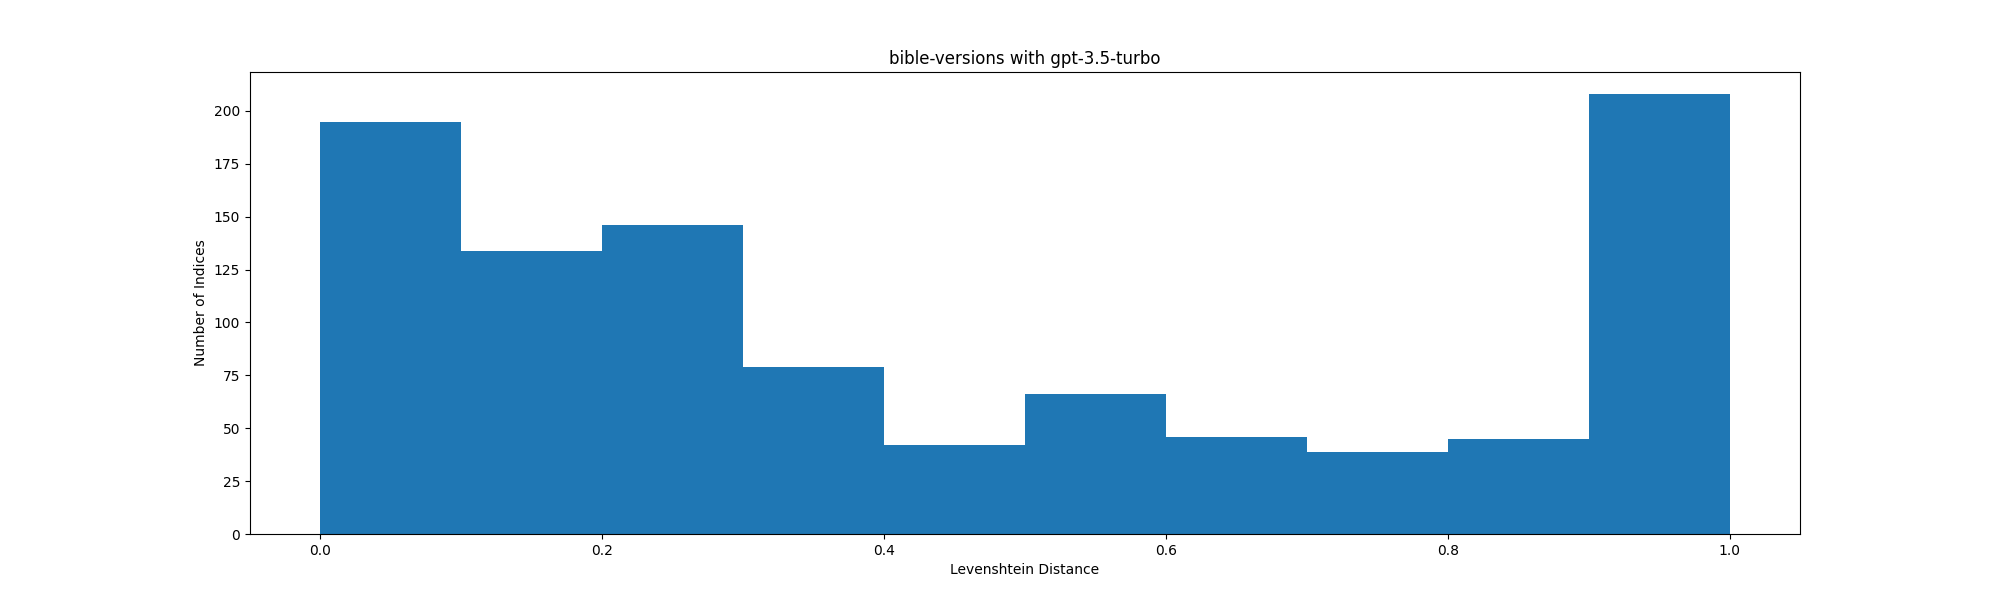
\includegraphics[width=1.0\textwidth]{bible-versions-gpt-3.5-turbo-histogram.png}  \\ 
% 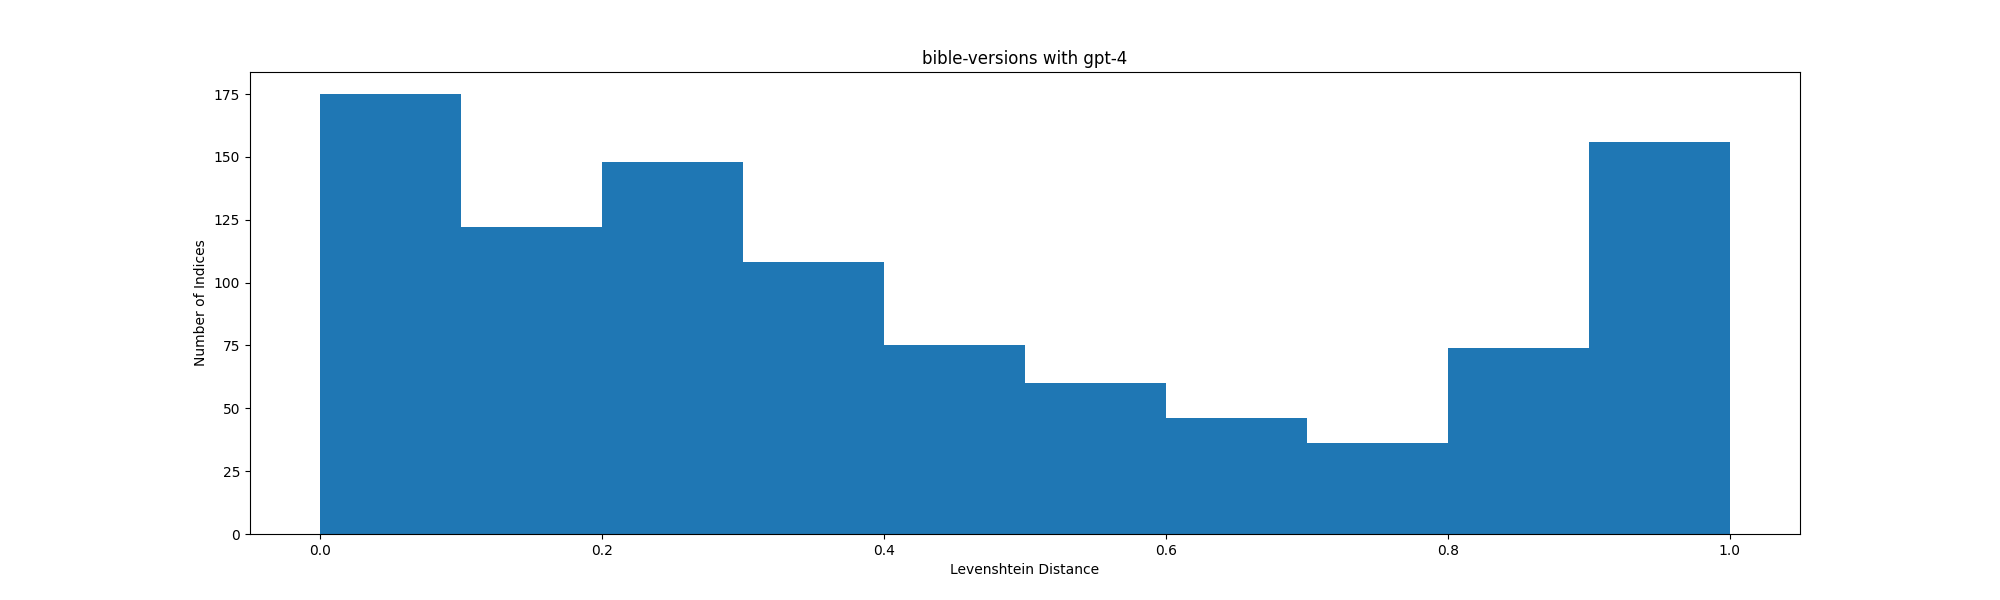
\includegraphics[width=1.0\textwidth]{bible-versions-gpt-4-histogram.png}  \\  
% 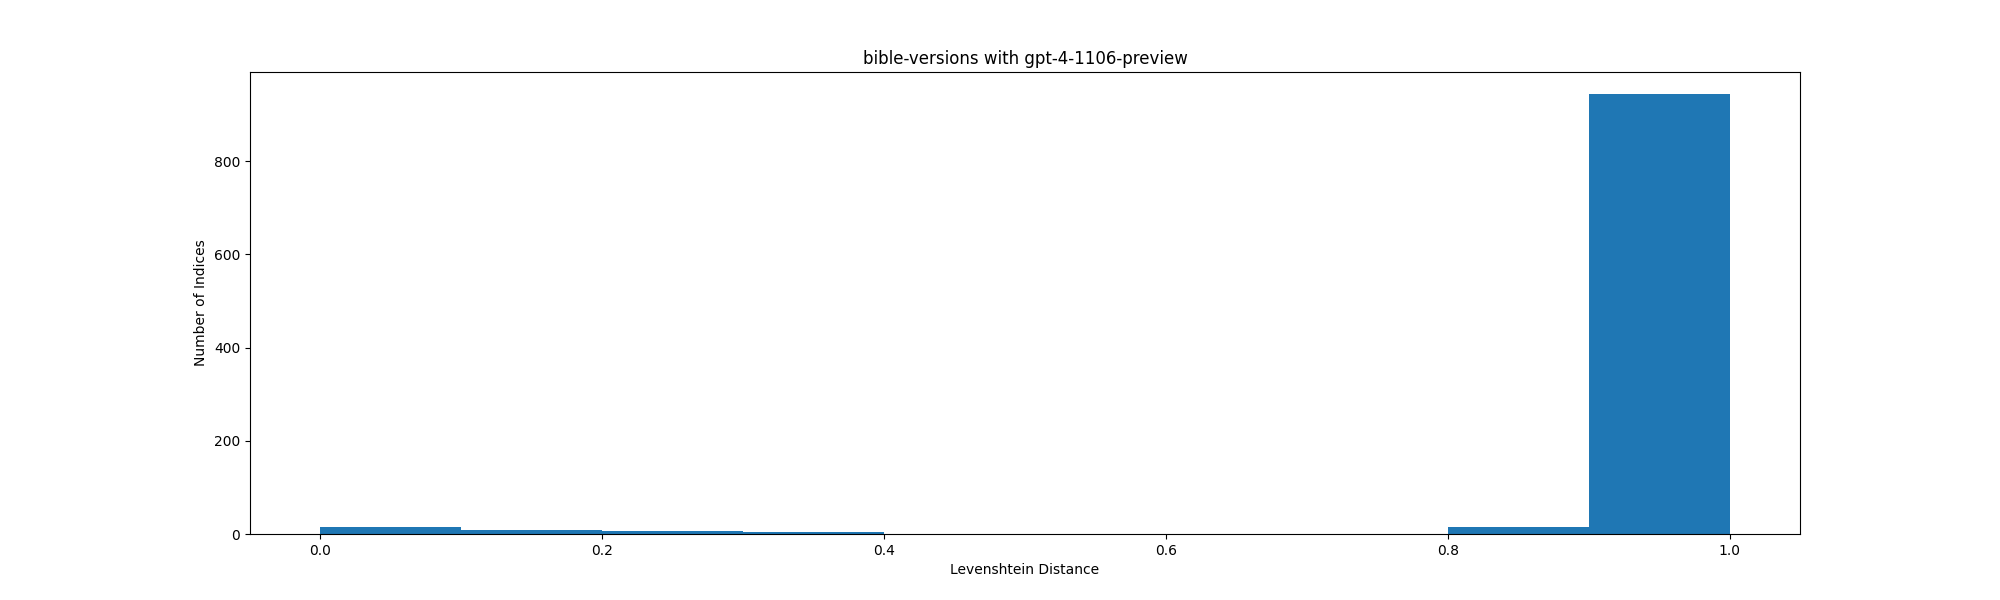
\includegraphics[width=1.0\textwidth]{bible-versions-gpt-4-1106-preview-histogram.png}  \\ 
% 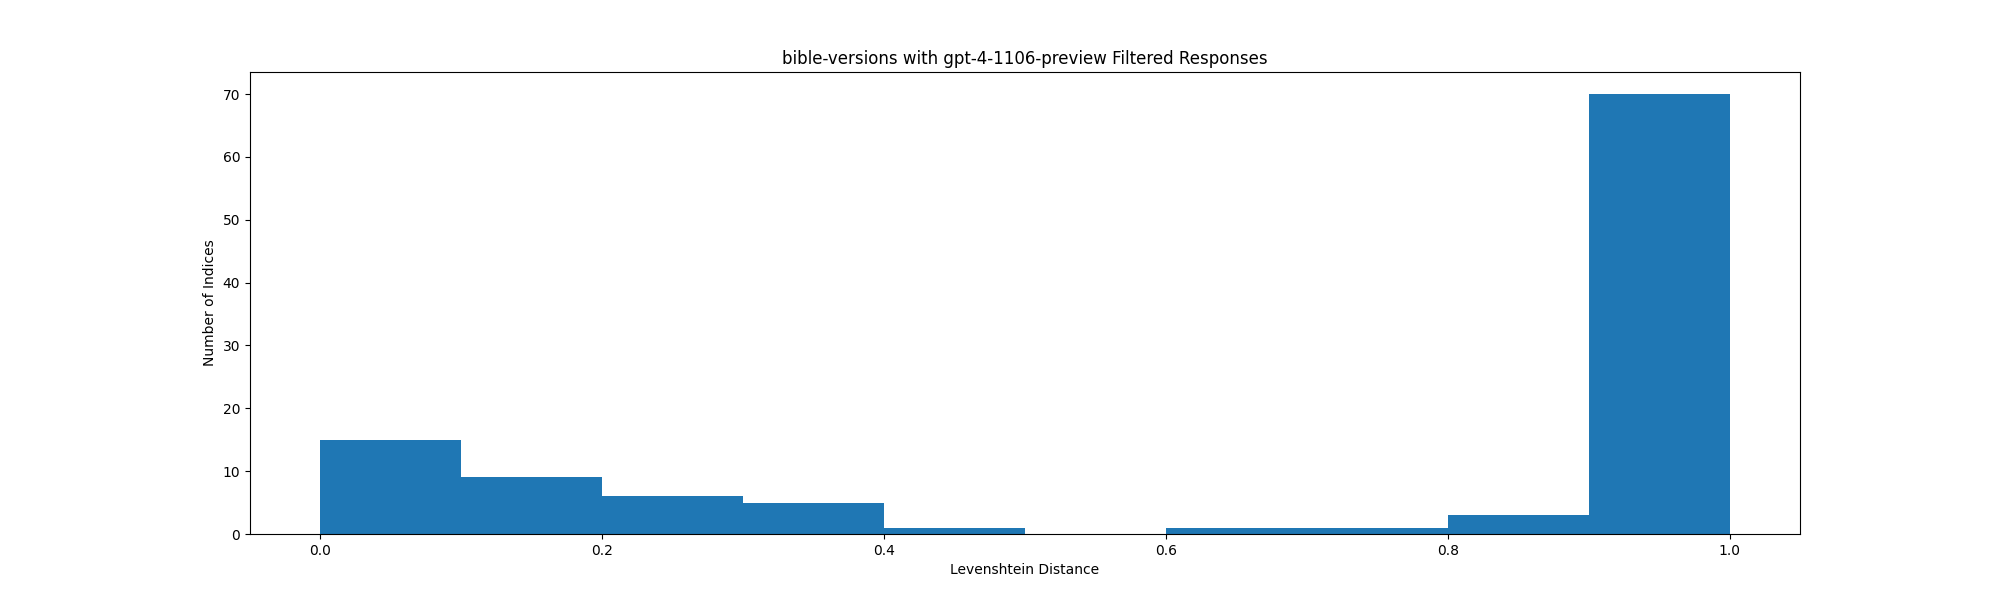
\includegraphics[width=1.0\textwidth]{bible-versions-gpt-4-1106-preview-histogram-filtered.png}  \\ 
% \end{tabular} 
% \caption{Levenshtein Distance Distribution for Bible Versions} 
% \label{tab:images} 
% \end{table} 



\begin{table}[ht] 
\centering 
\begin{tabular}{c}  
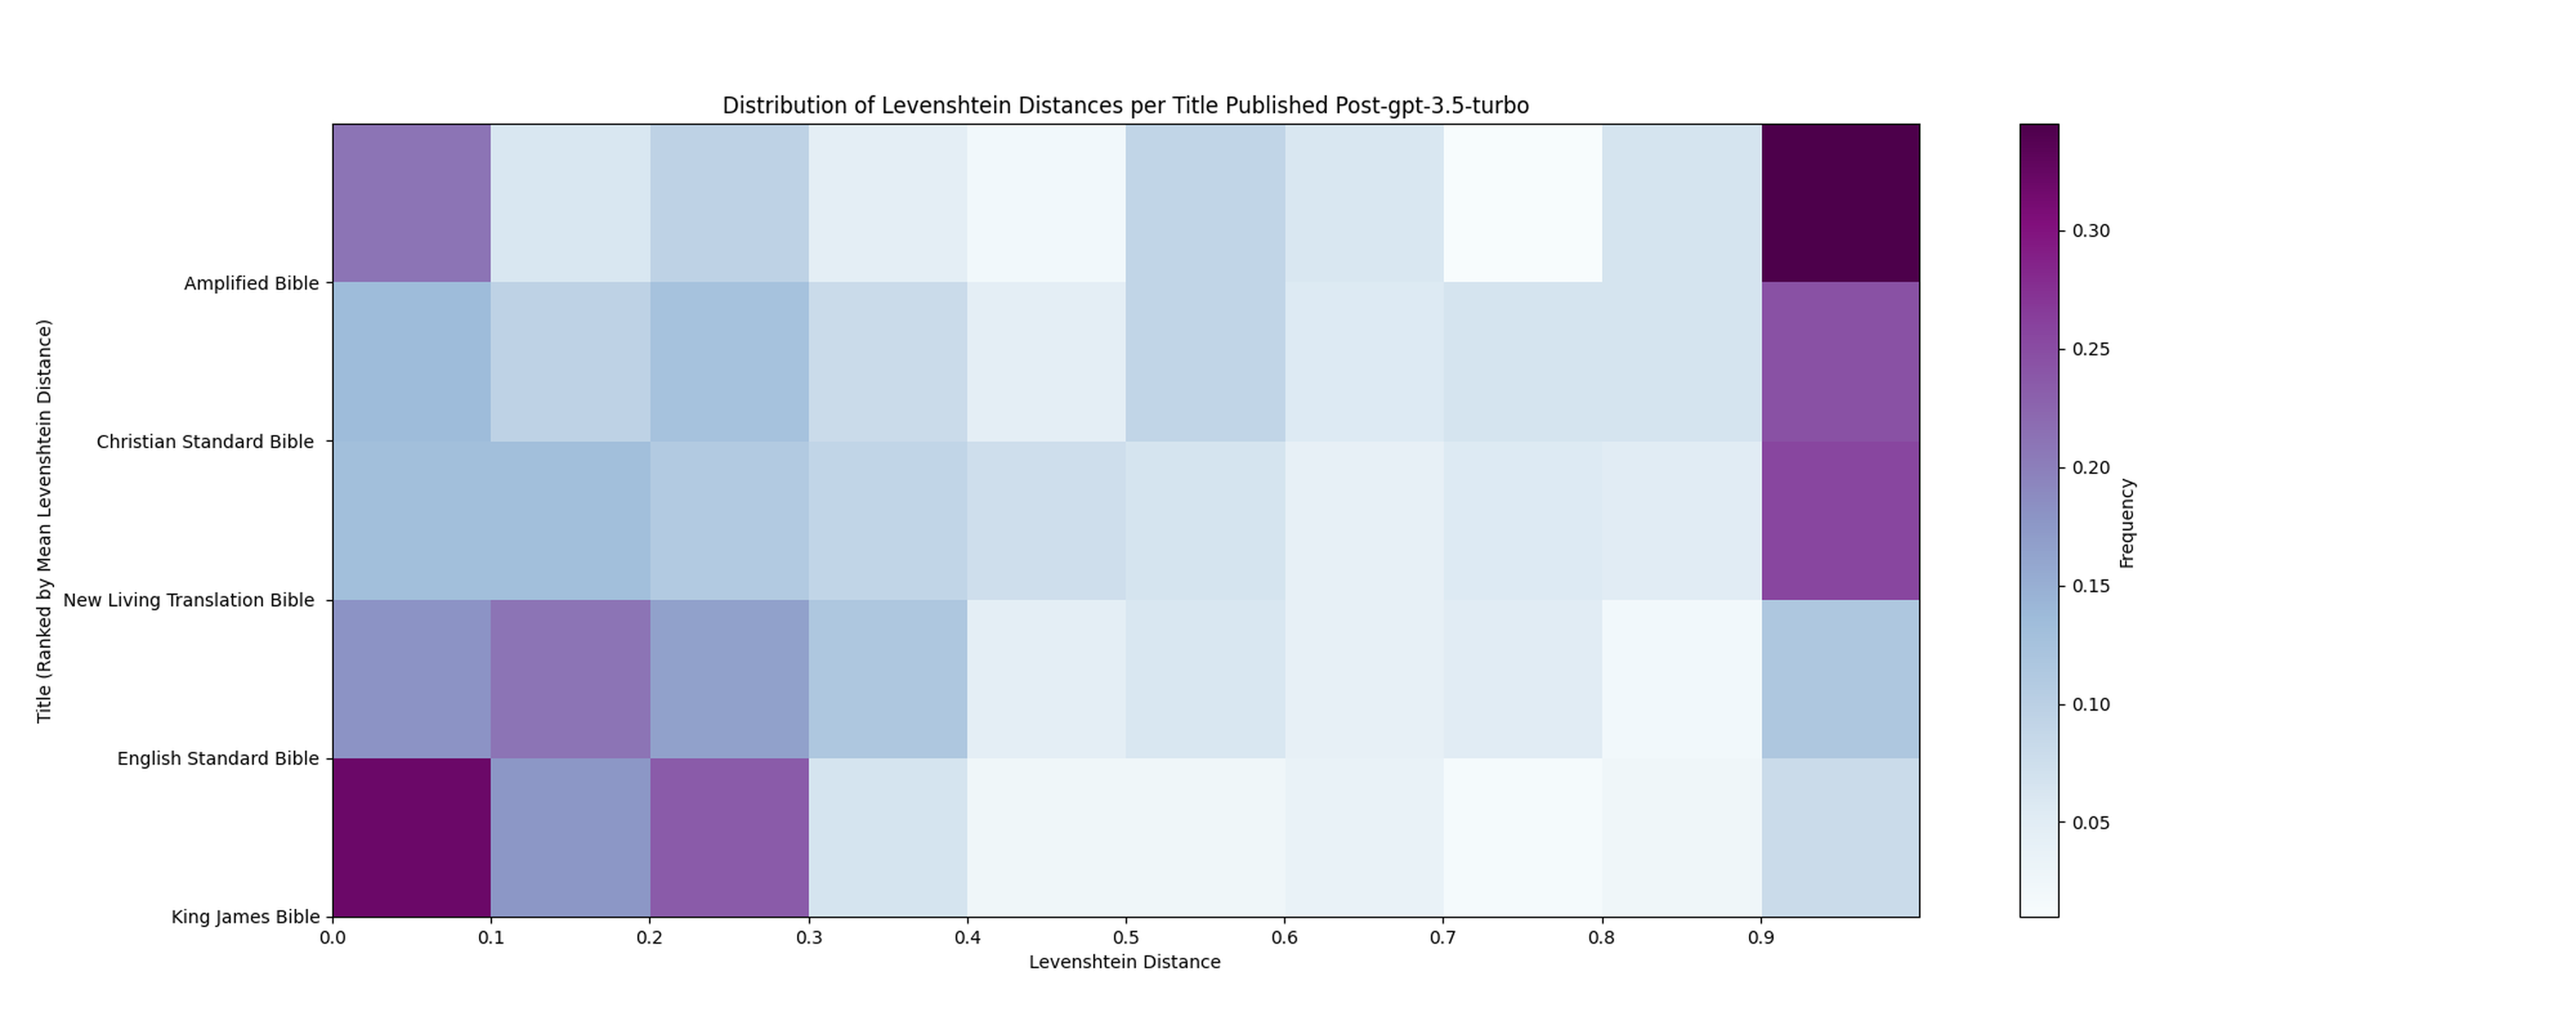
\includegraphics[width=1.0\textwidth]{plots/bible-versions-gpt-3.5-turbo-2d-histogram.png}  \\  
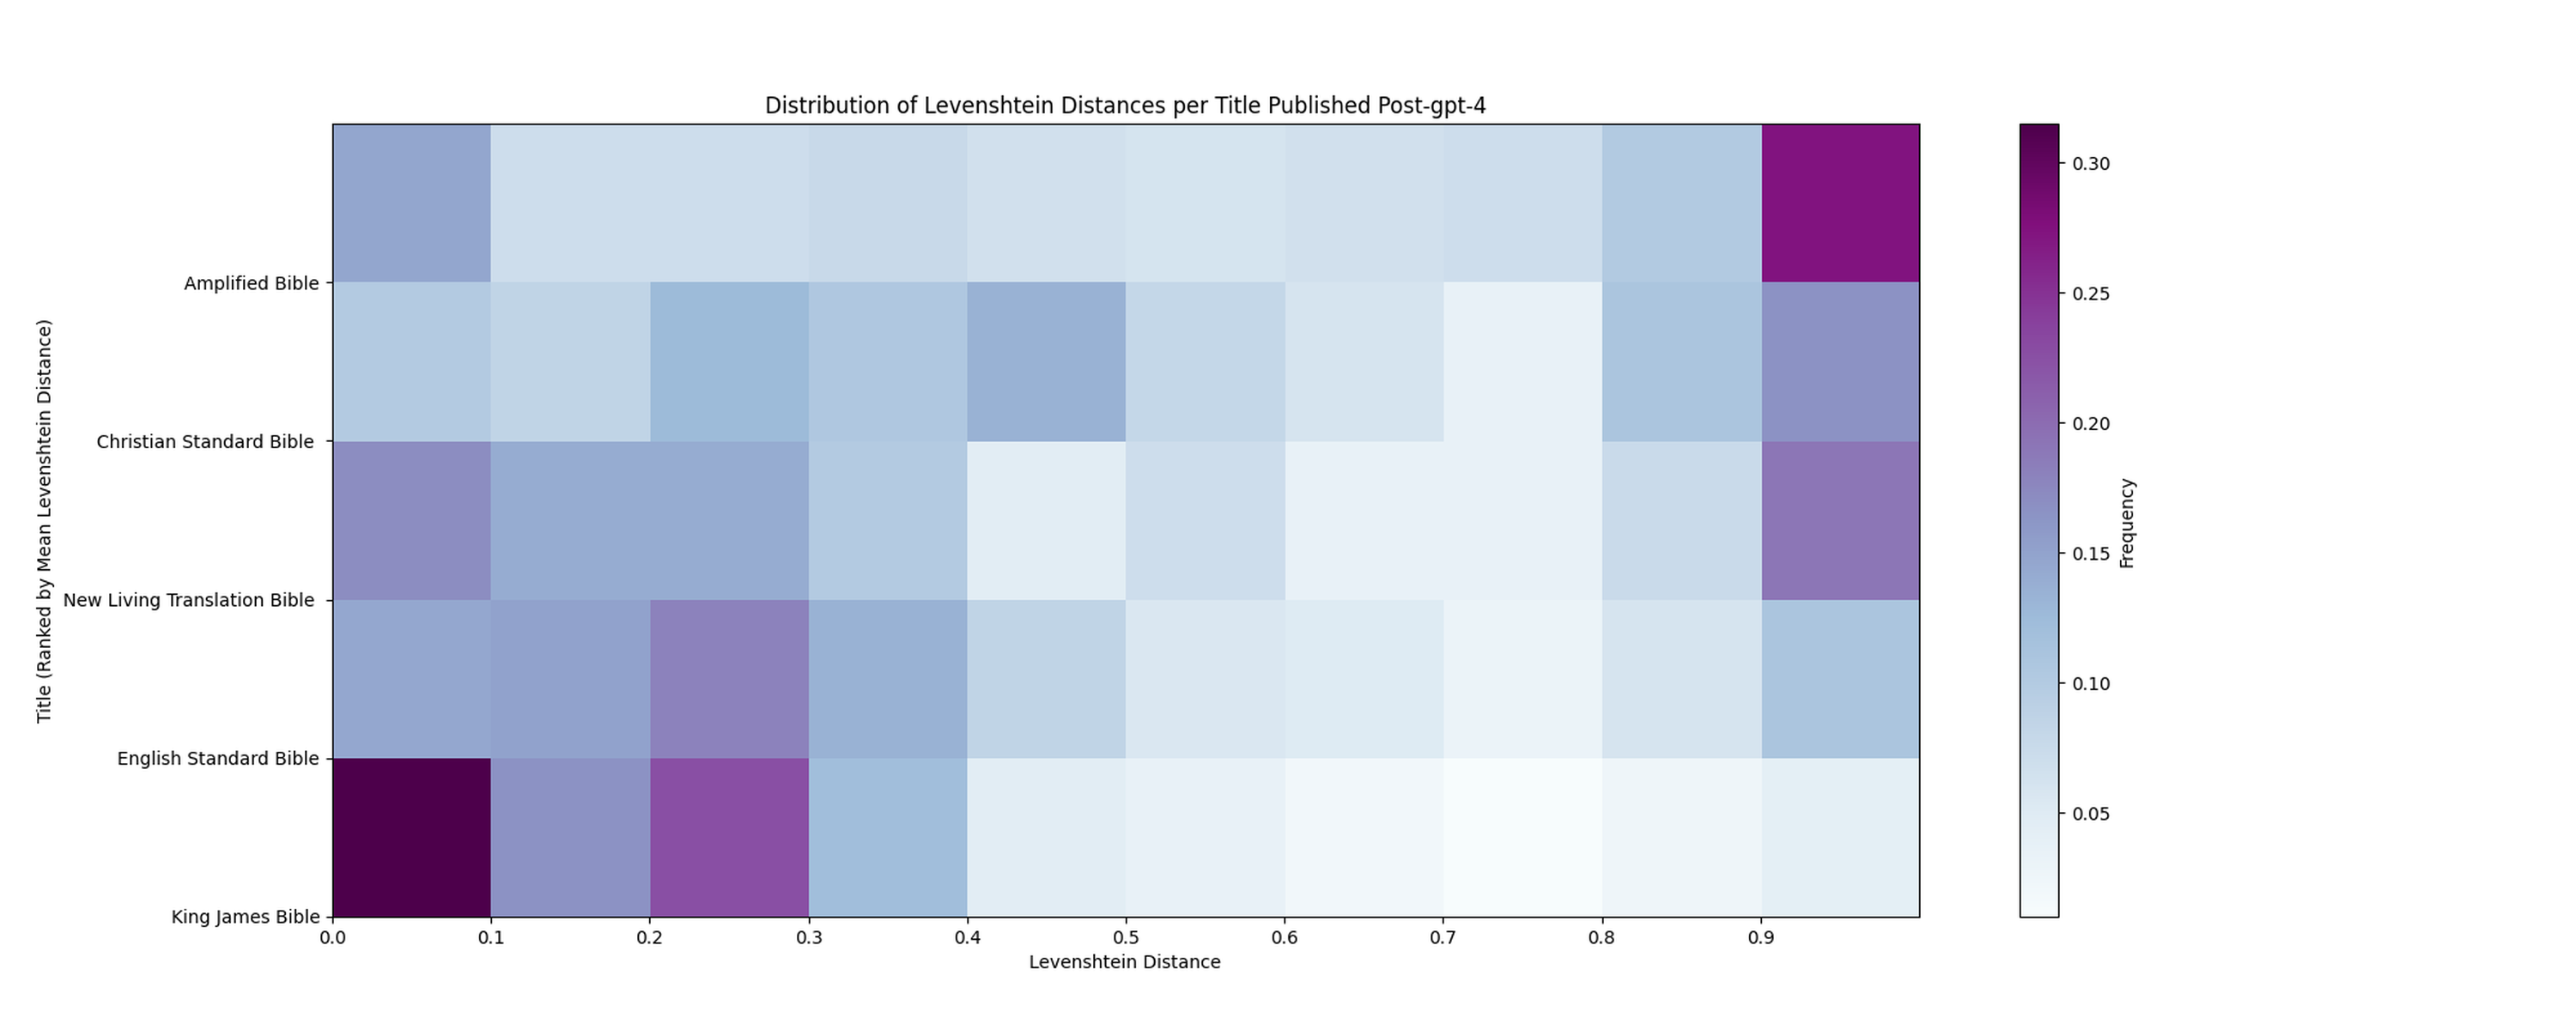
\includegraphics[width=1.0\textwidth]{plots/bible-versions-gpt-4-2d-histogram.png}  \\  
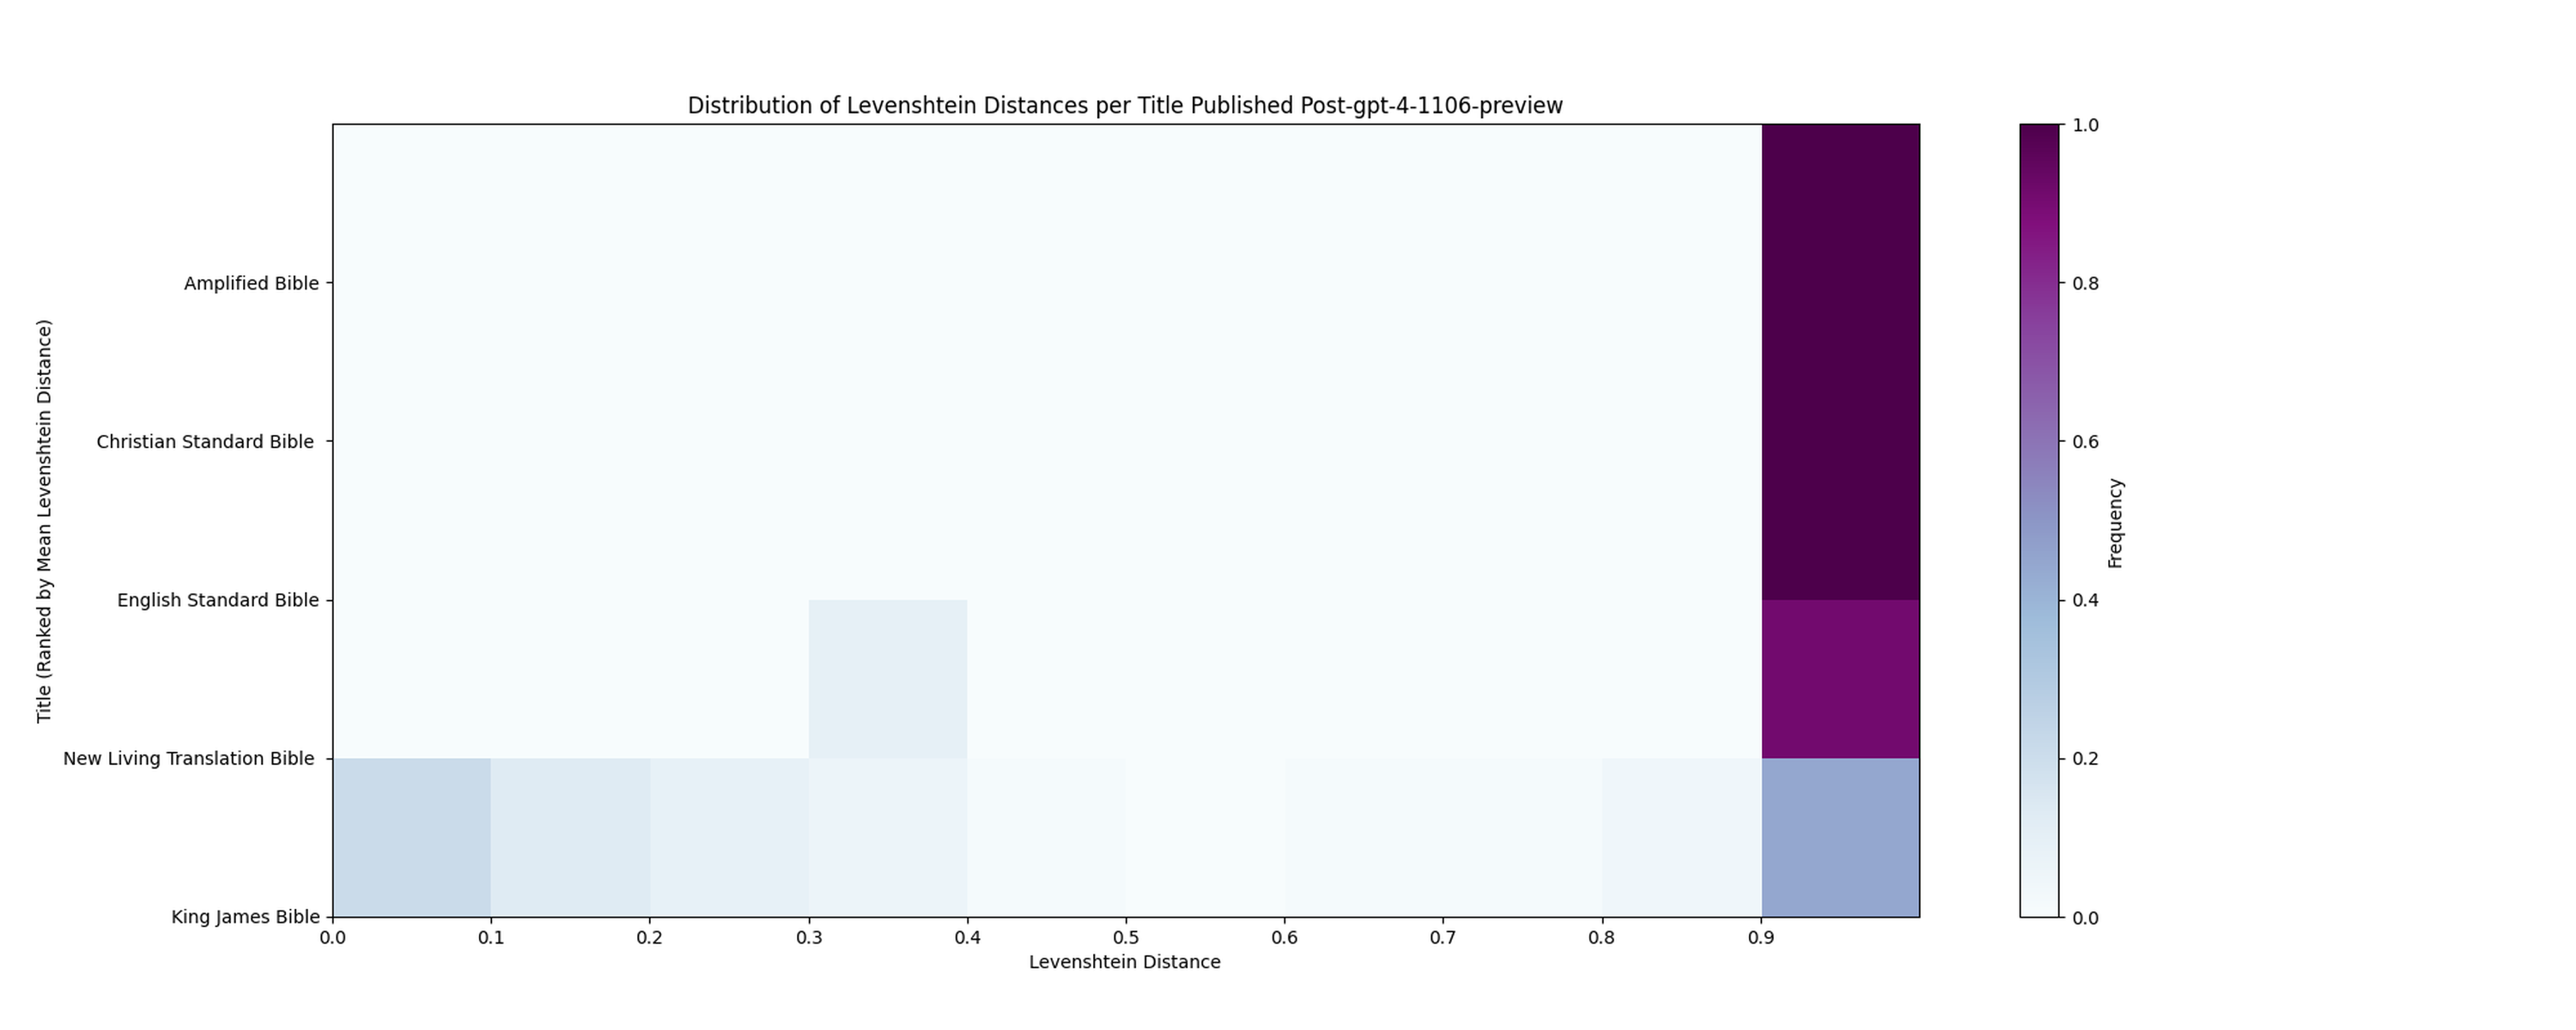
\includegraphics[width=1.0\textwidth]{plots/bible-versions-gpt-4-1106-preview-2d-histogram.png}  \\  
\end{tabular} 
\caption{Levenshtein Distance Distribution per Types of Bible Versions} 
\label{tab:images} 
\end{table} 



% \begin{table}[ht] 
% \centering 
% \begin{tabular}{c} 
% 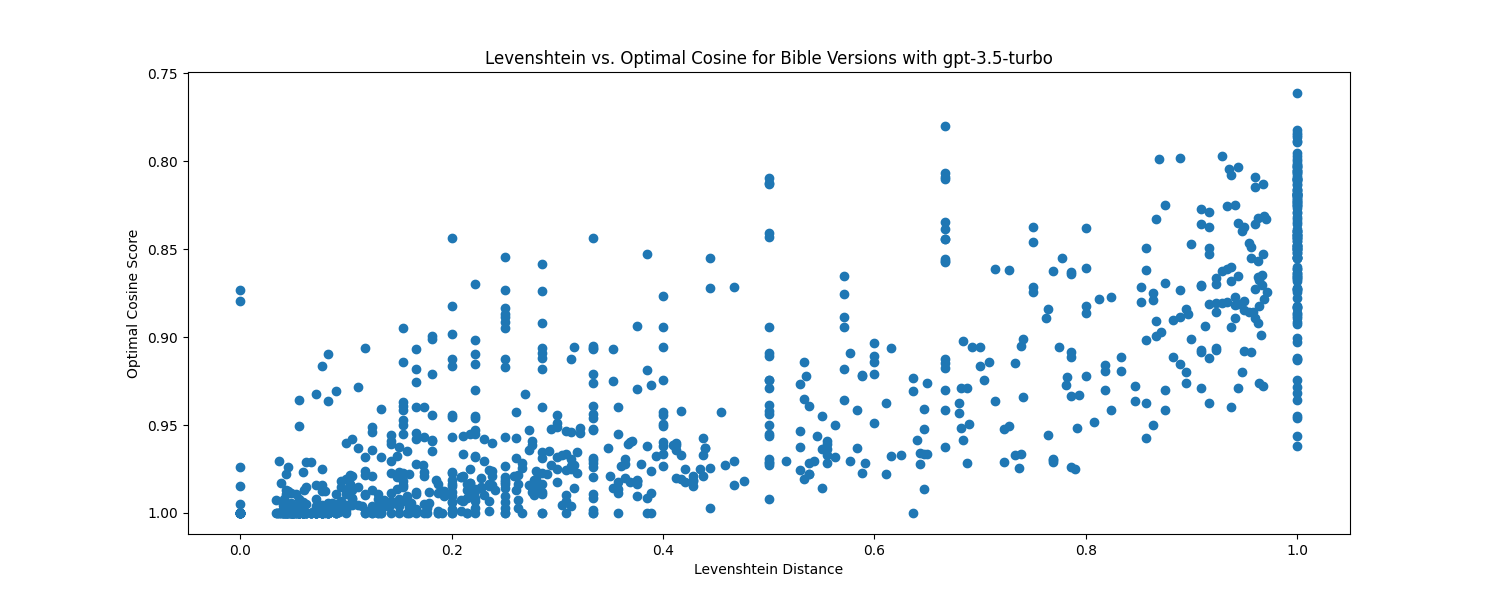
\includegraphics[width=1.0\textwidth]{bible-versions_levenshtein_v_cosine-gpt-3.5-turbo.png}  \\  
% 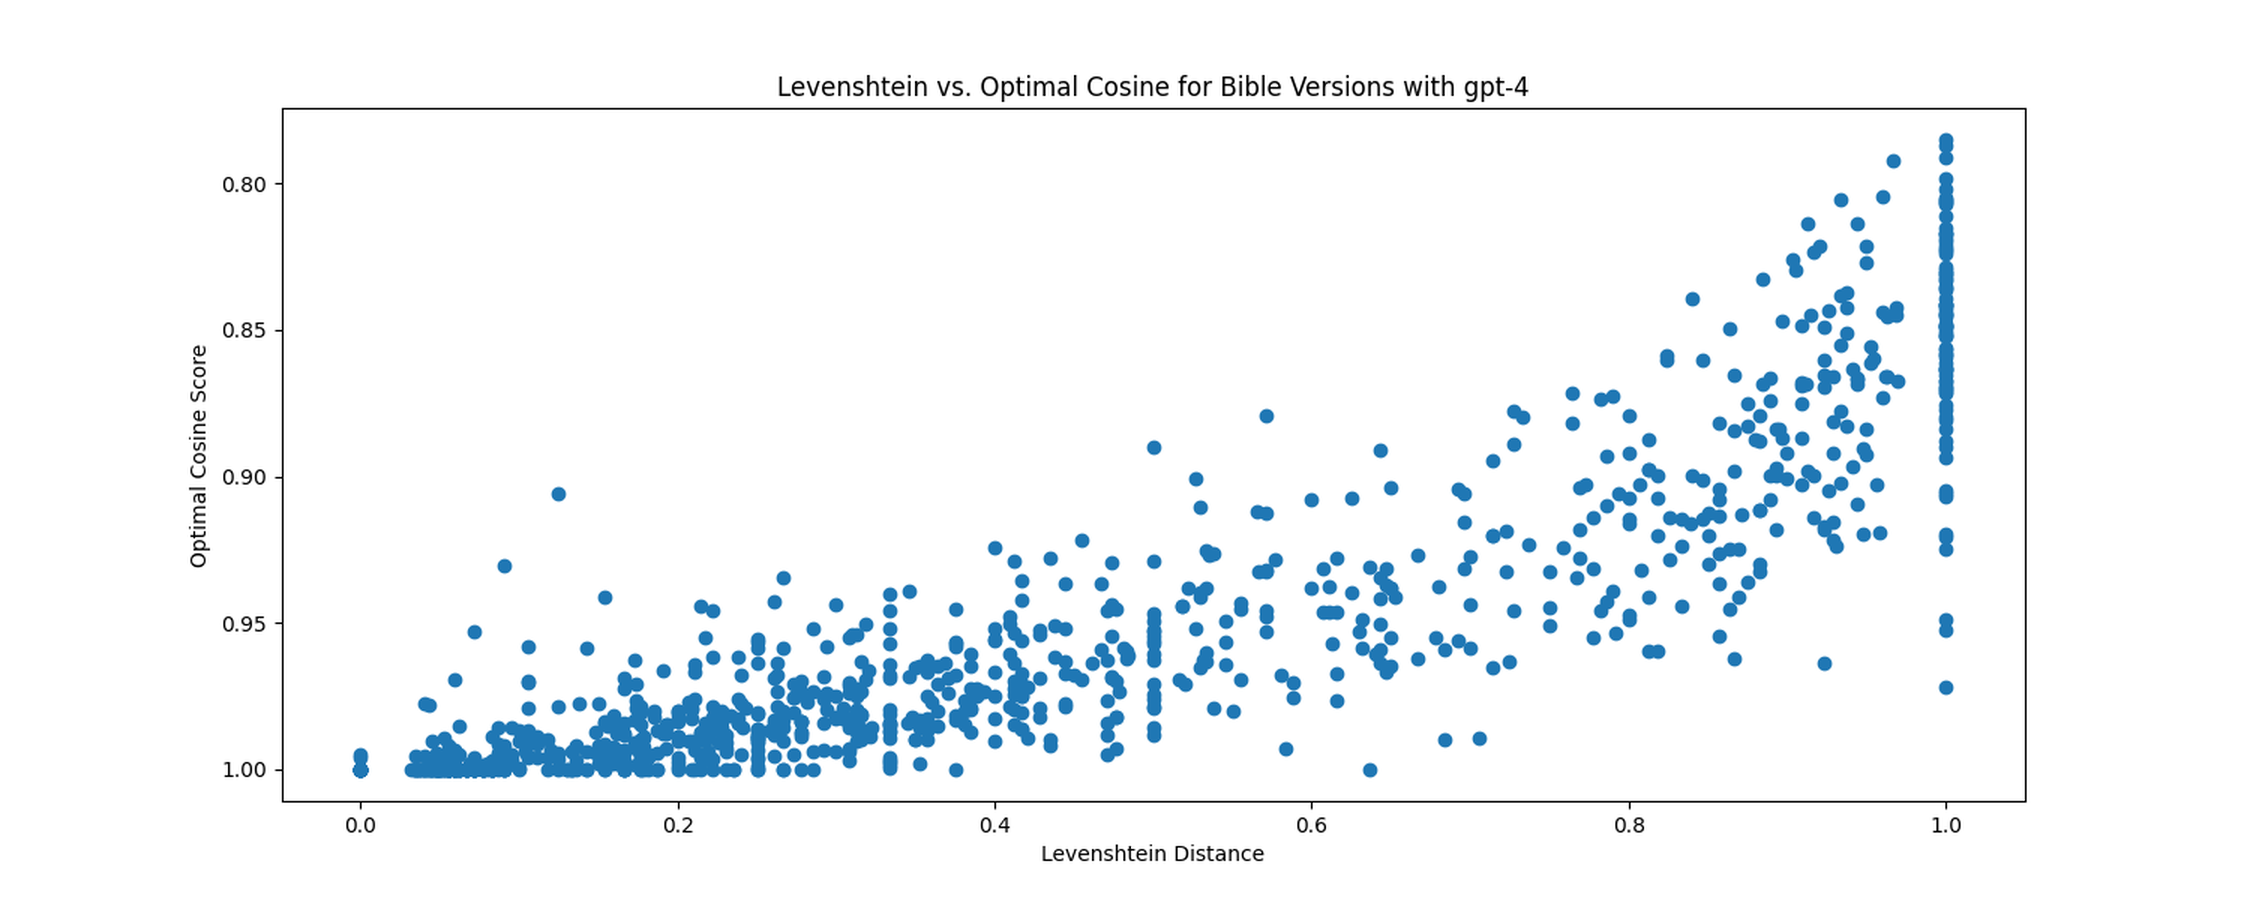
\includegraphics[width=1.0\textwidth]{bible-versions_levenshtein_v_cosine-gpt-4.png}  \\  
% 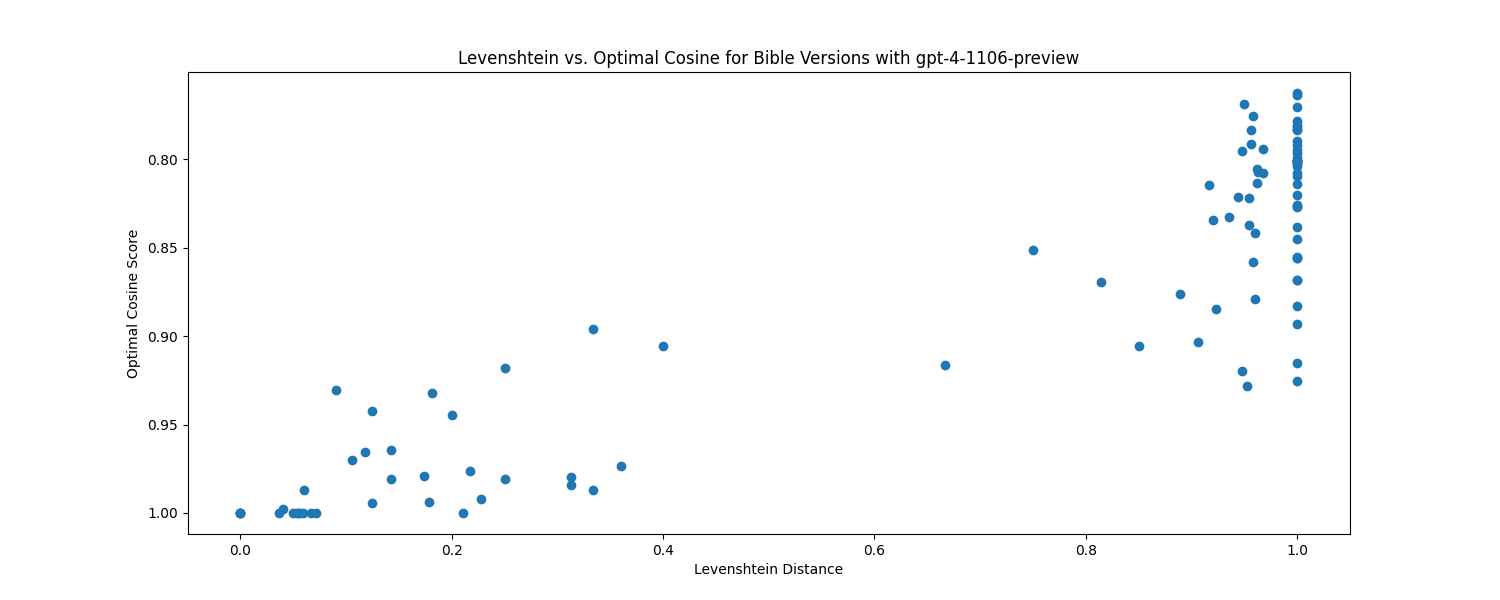
\includegraphics[width=1.0\textwidth]{bible-versions_levenshtein_v_cosine-gpt-4-1106-preview.png}  \\ 
% \end{tabular} 
% \caption{Levenshtein vs. Cosine Similarity Score for Bible Versions} 
% \label{tab:images} 
% \end{table} 

% \begin{table}[ht] 
% \centering 
% \begin{tabular}{c} 
% 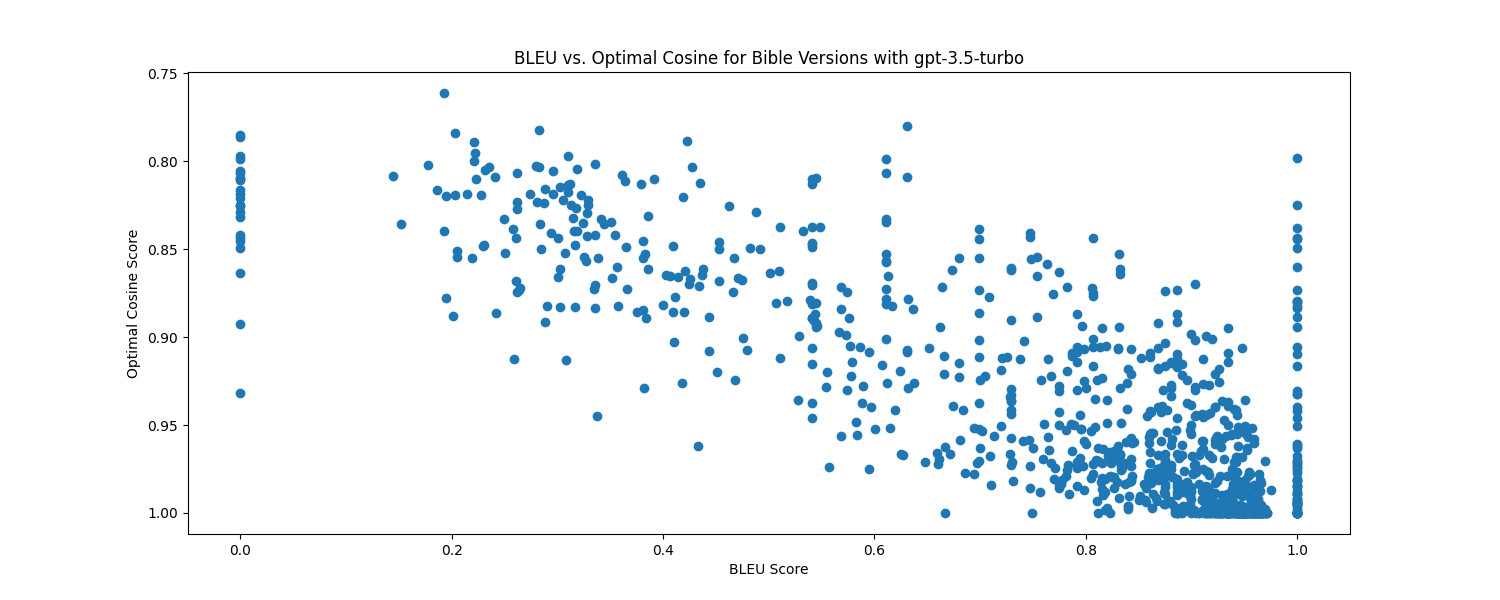
\includegraphics[width=1.0\textwidth]{bible-versions_bleu_v_cosine-gpt-3.5-turbo.png}  \\  
% 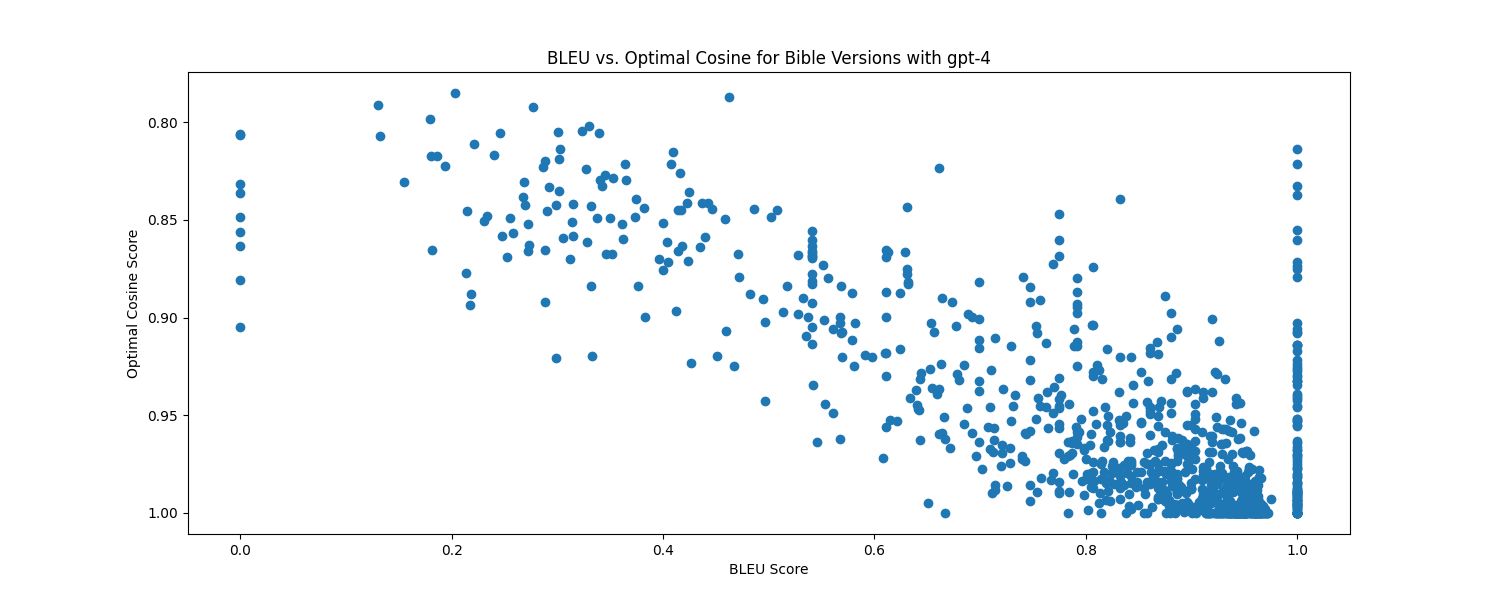
\includegraphics[width=1.0\textwidth]{bible-versions_bleu_v_cosine-gpt-4.png}  \\  
% 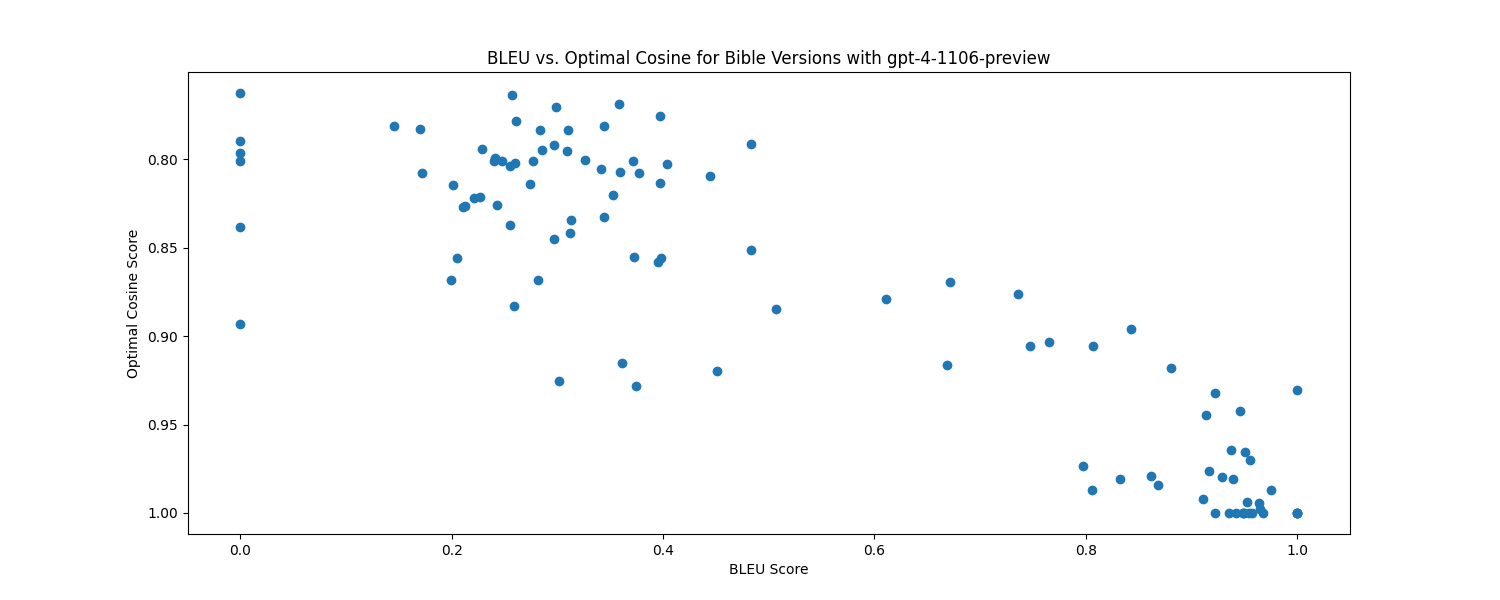
\includegraphics[width=1.0\textwidth]{bible-versions_bleu_v_cosine-gpt-4-1106-preview.png}  \\ 
% \end{tabular} 
% \caption{Bleu vs. Cosine Similarity Score for Bible Versions} 
% \label{tab:images} 
% \end{table} 

% \begin{table}[ht] 
% \centering 
% \begin{tabular}{c} 
% 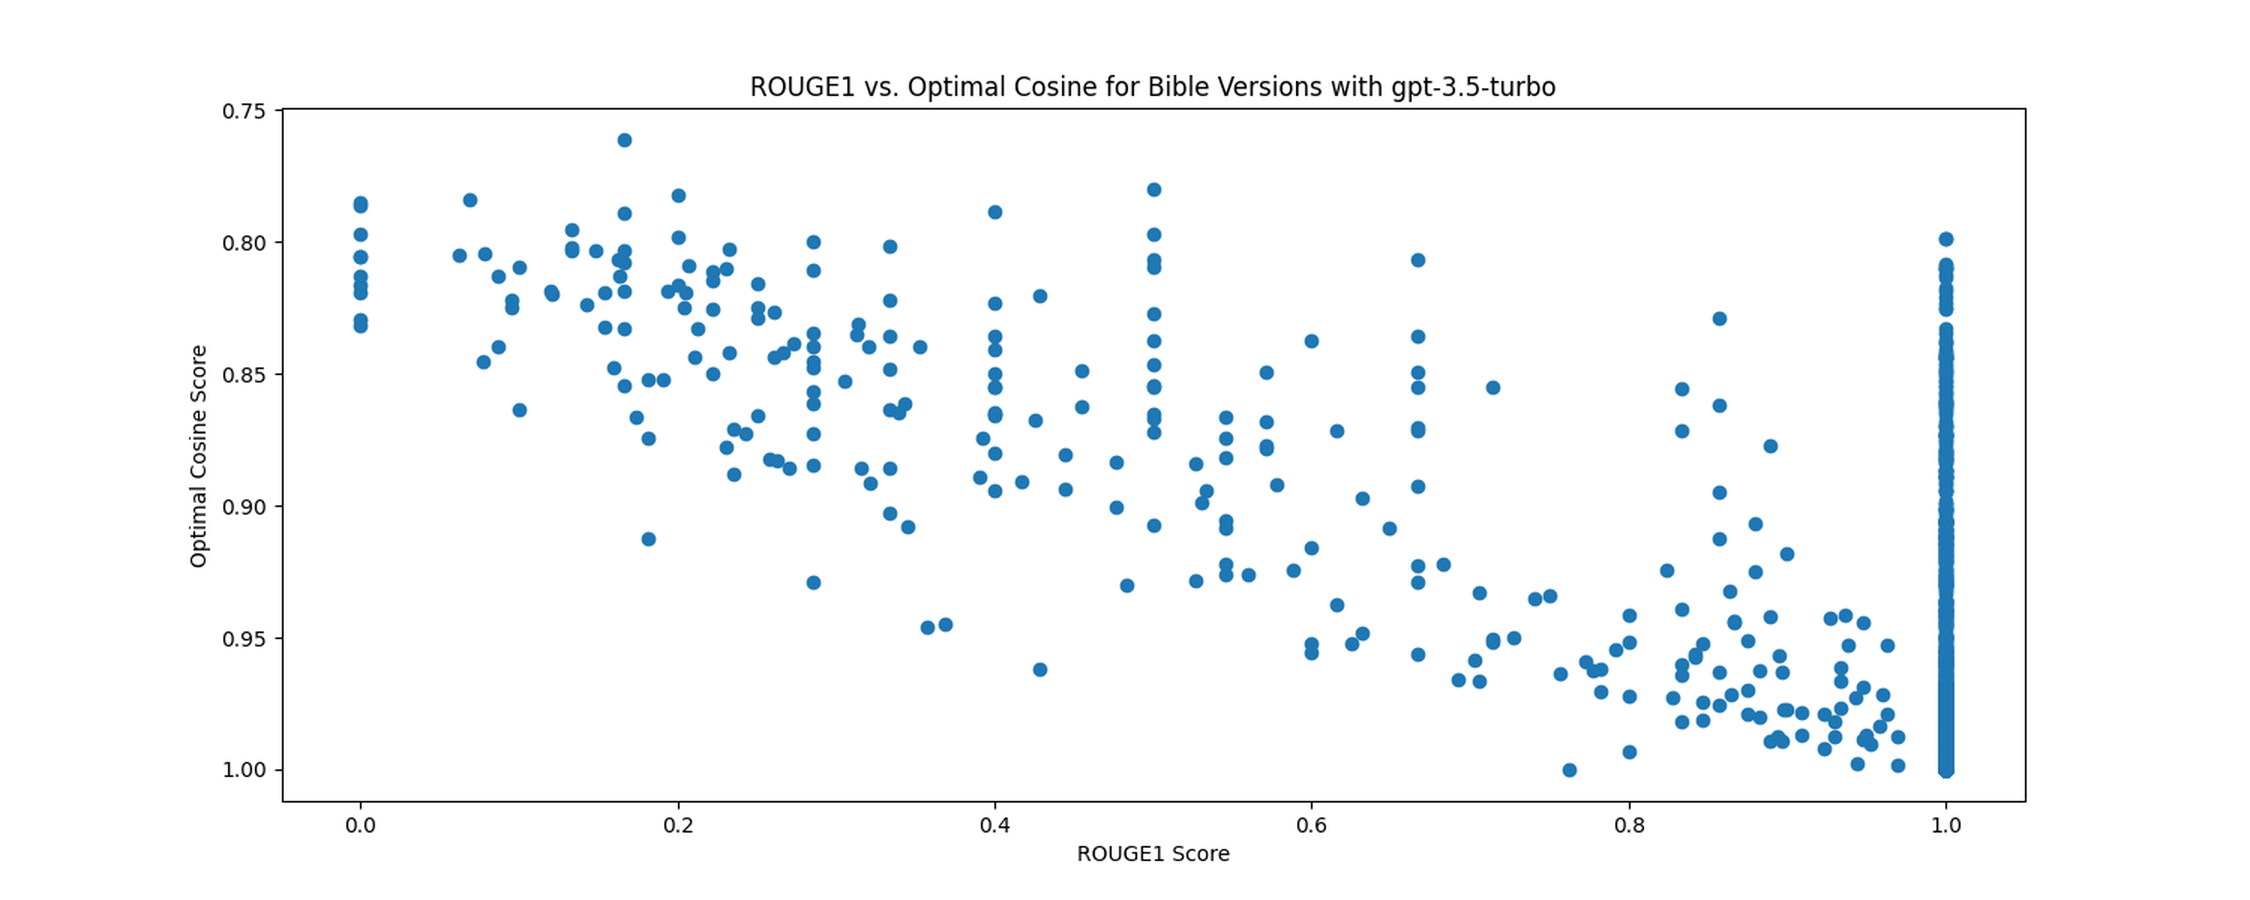
\includegraphics[width=1.0\textwidth]{bible-versions_rouge1_v_cosine-gpt-3.5-turbo.png}  \\  
% 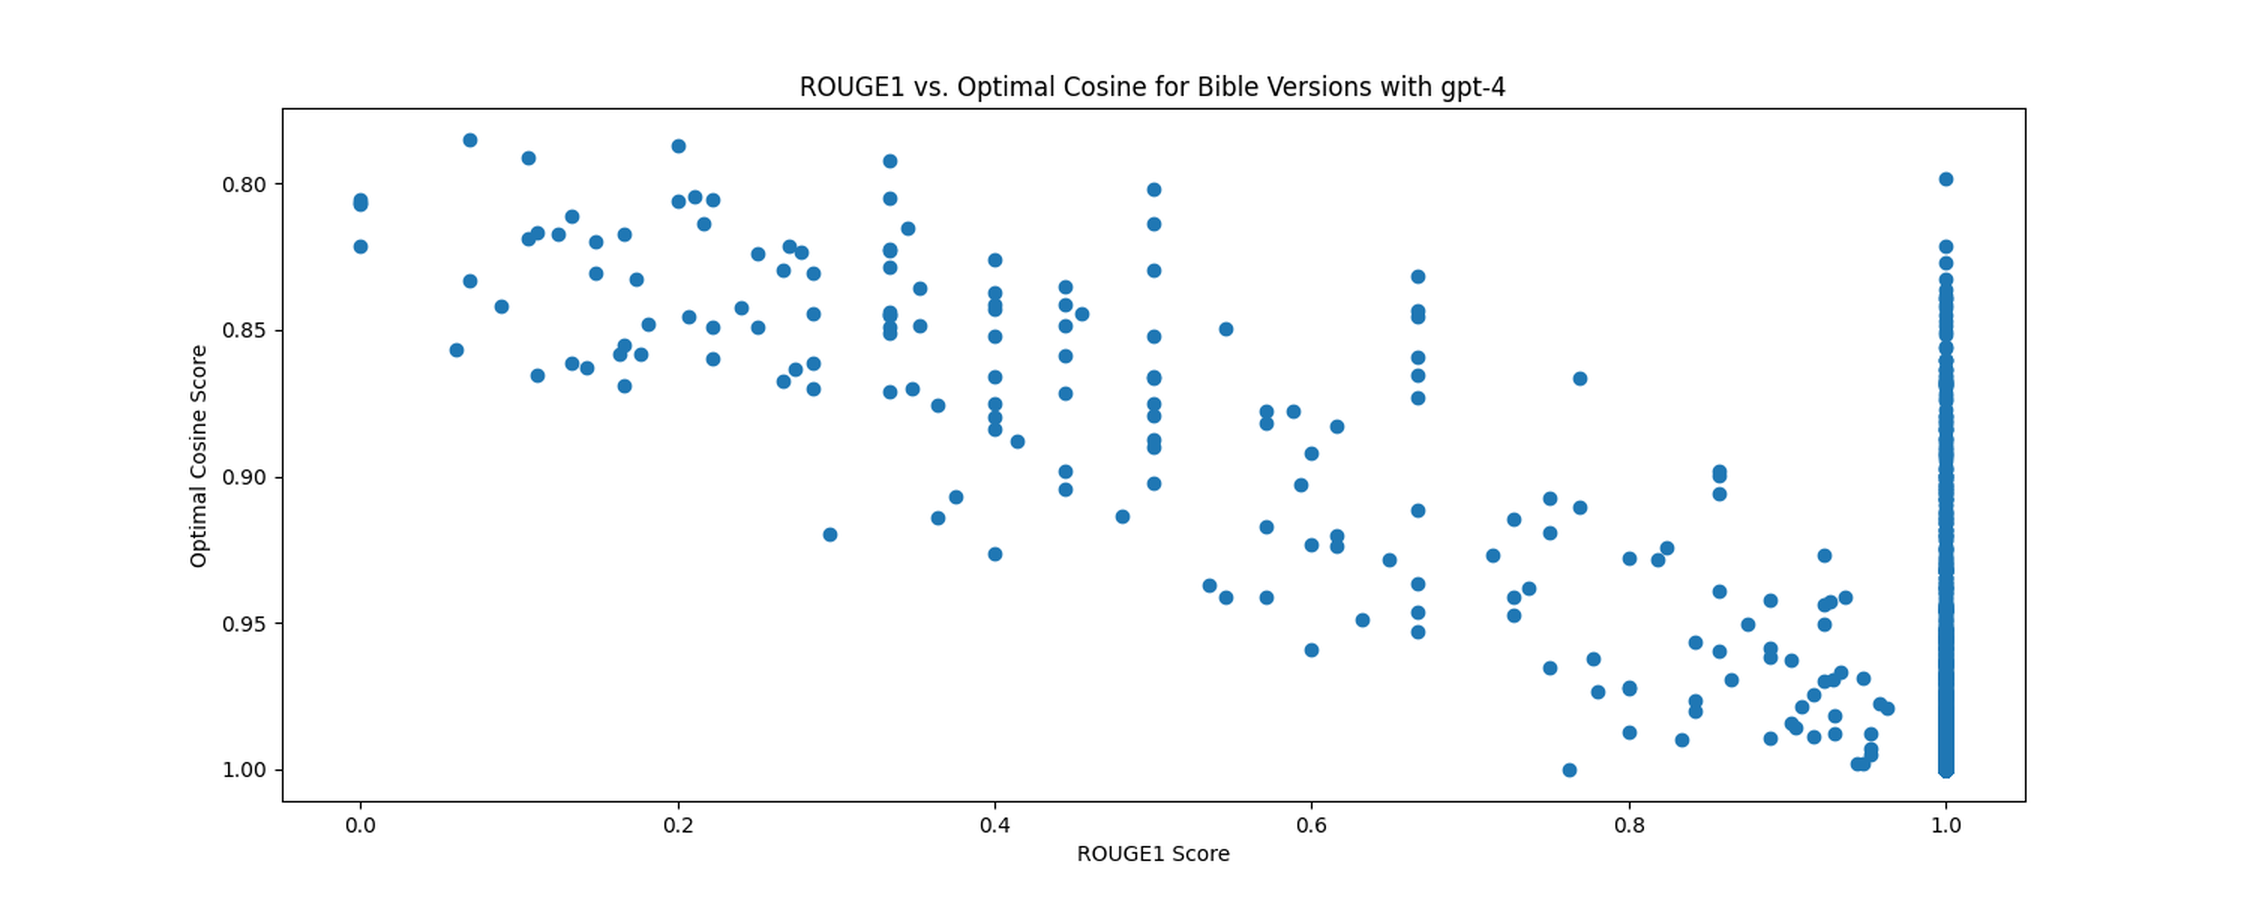
\includegraphics[width=1.0\textwidth]{bible-versions_rouge1_v_cosine-gpt-4.png}  \\  
% 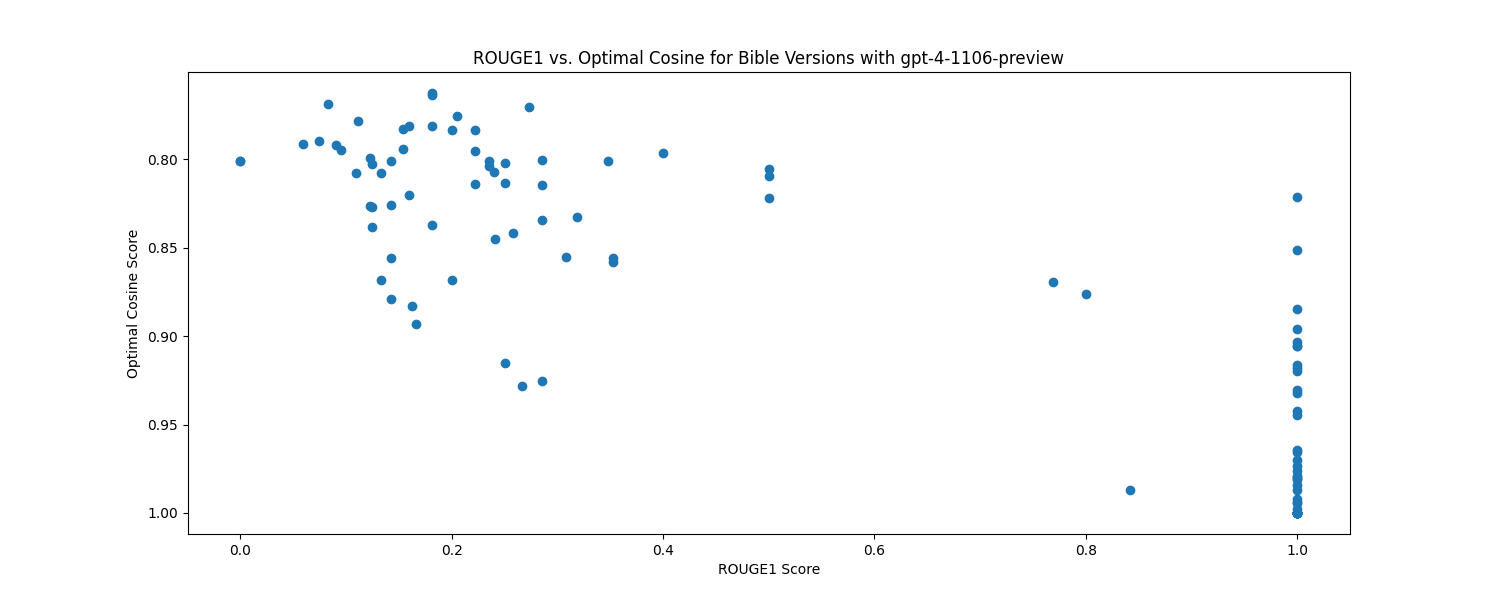
\includegraphics[width=1.0\textwidth]{bible-versions_rouge1_v_cosine-gpt-4-1106-preview.png}  \\ 
% \end{tabular} 
% \caption{Rouge1 vs. Cosine Similarity Score for Bible Versions} 
% \label{tab:images} 
% \end{table} 

% \begin{table}[ht] 
% \centering 
% \begin{tabular}{c} 
% 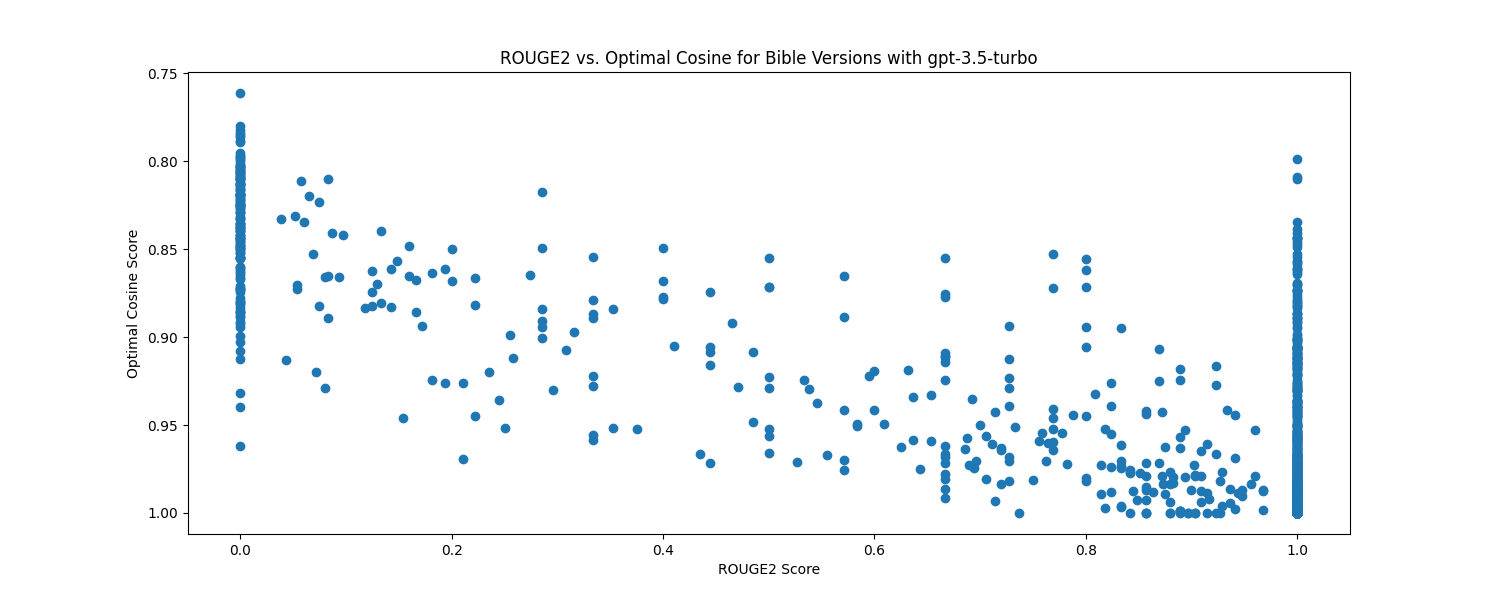
\includegraphics[width=1.0\textwidth]{bible-versions_rouge2_v_cosine-gpt-3.5-turbo.png}  \\  
% 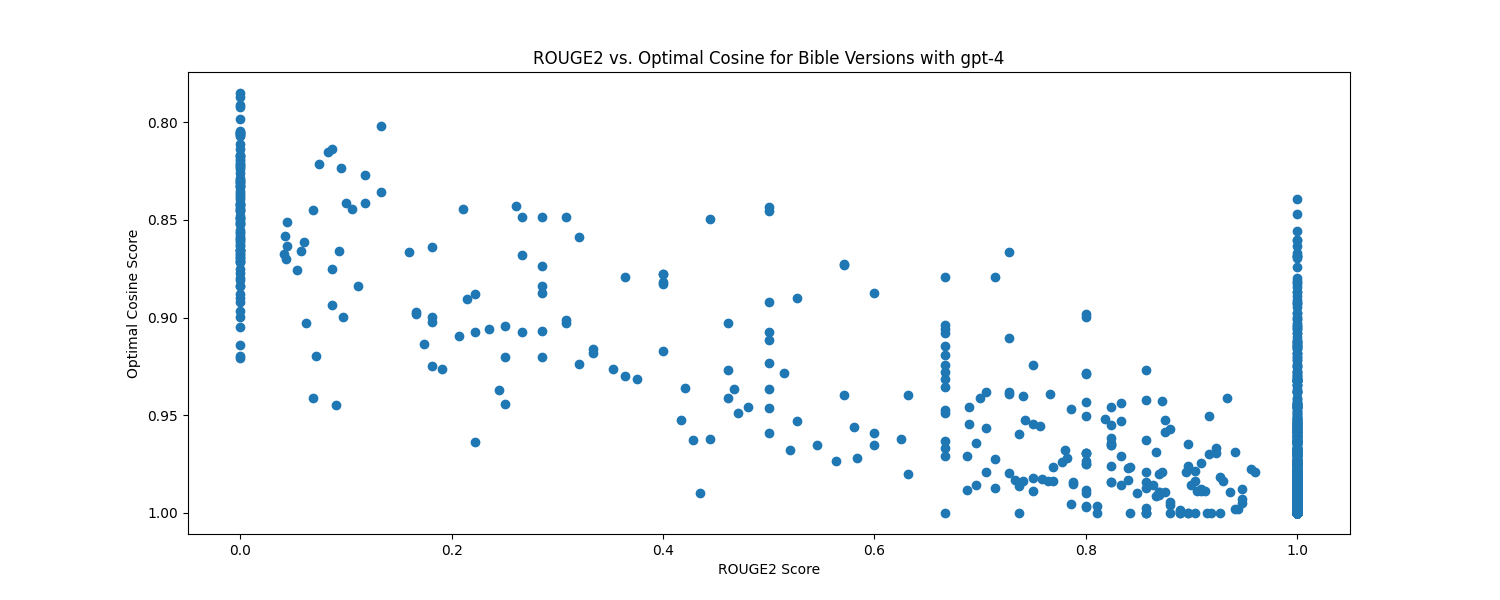
\includegraphics[width=1.0\textwidth]{bible-versions_rouge2_v_cosine-gpt-4.png}  \\  
% 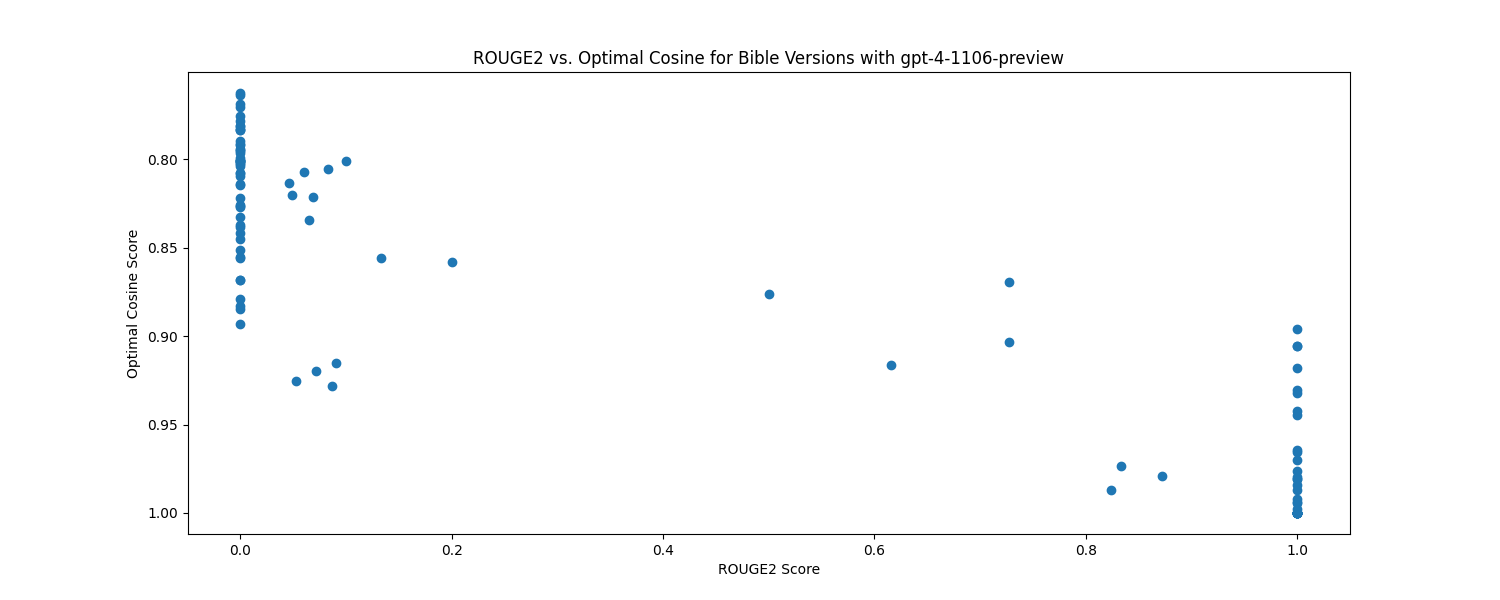
\includegraphics[width=1.0\textwidth]{bible-versions_rouge2_v_cosine-gpt-4-1106-preview.png}  \\ 
% \end{tabular} 
% \caption{Rouge2 vs. Cosine Similarity Score for Bible Versions} 
% \label{tab:images} 
% \end{table} 


% \begin{table}[ht] 
% \centering 
% \begin{tabular}{c} 
% 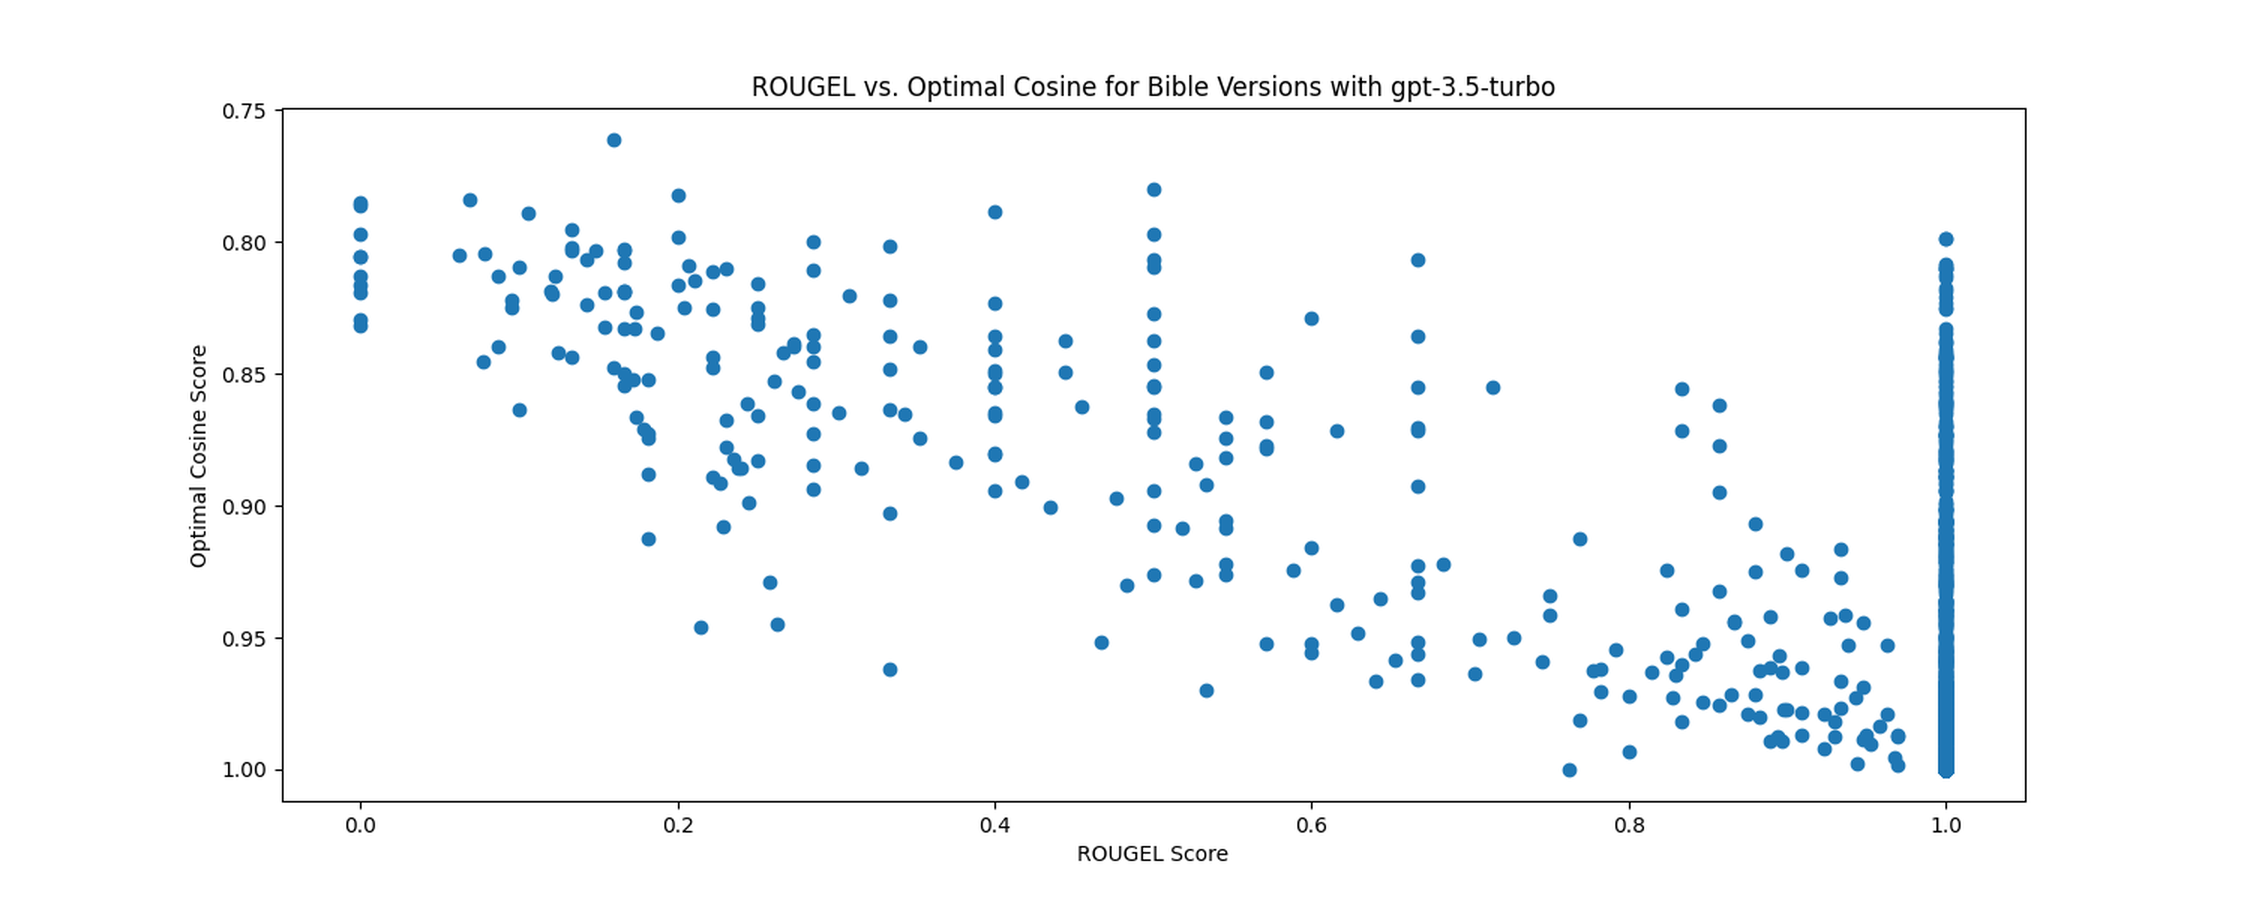
\includegraphics[width=1.0\textwidth]{bible-versions_rougeL_v_cosine-gpt-3.5-turbo.png}  \\  
% 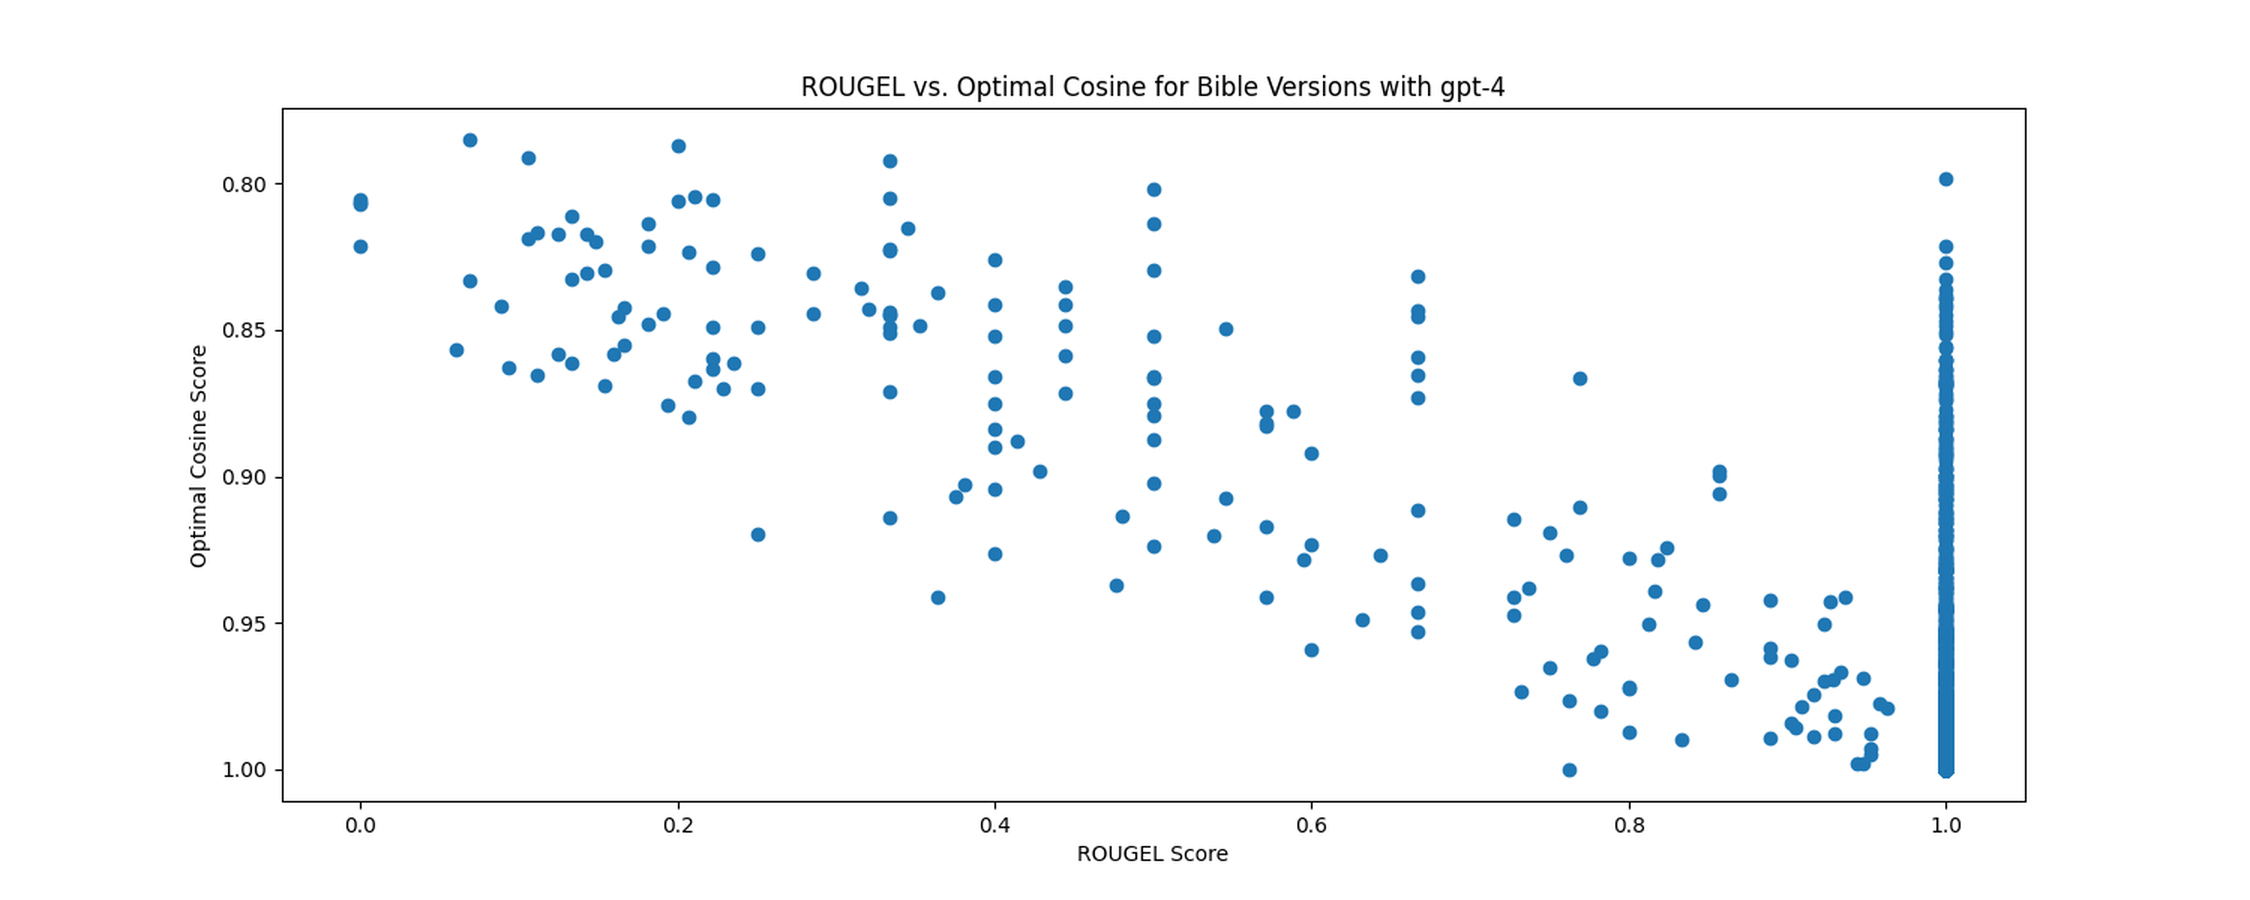
\includegraphics[width=1.0\textwidth]{bible-versions_rougeL_v_cosine-gpt-4.png}  \\  
% 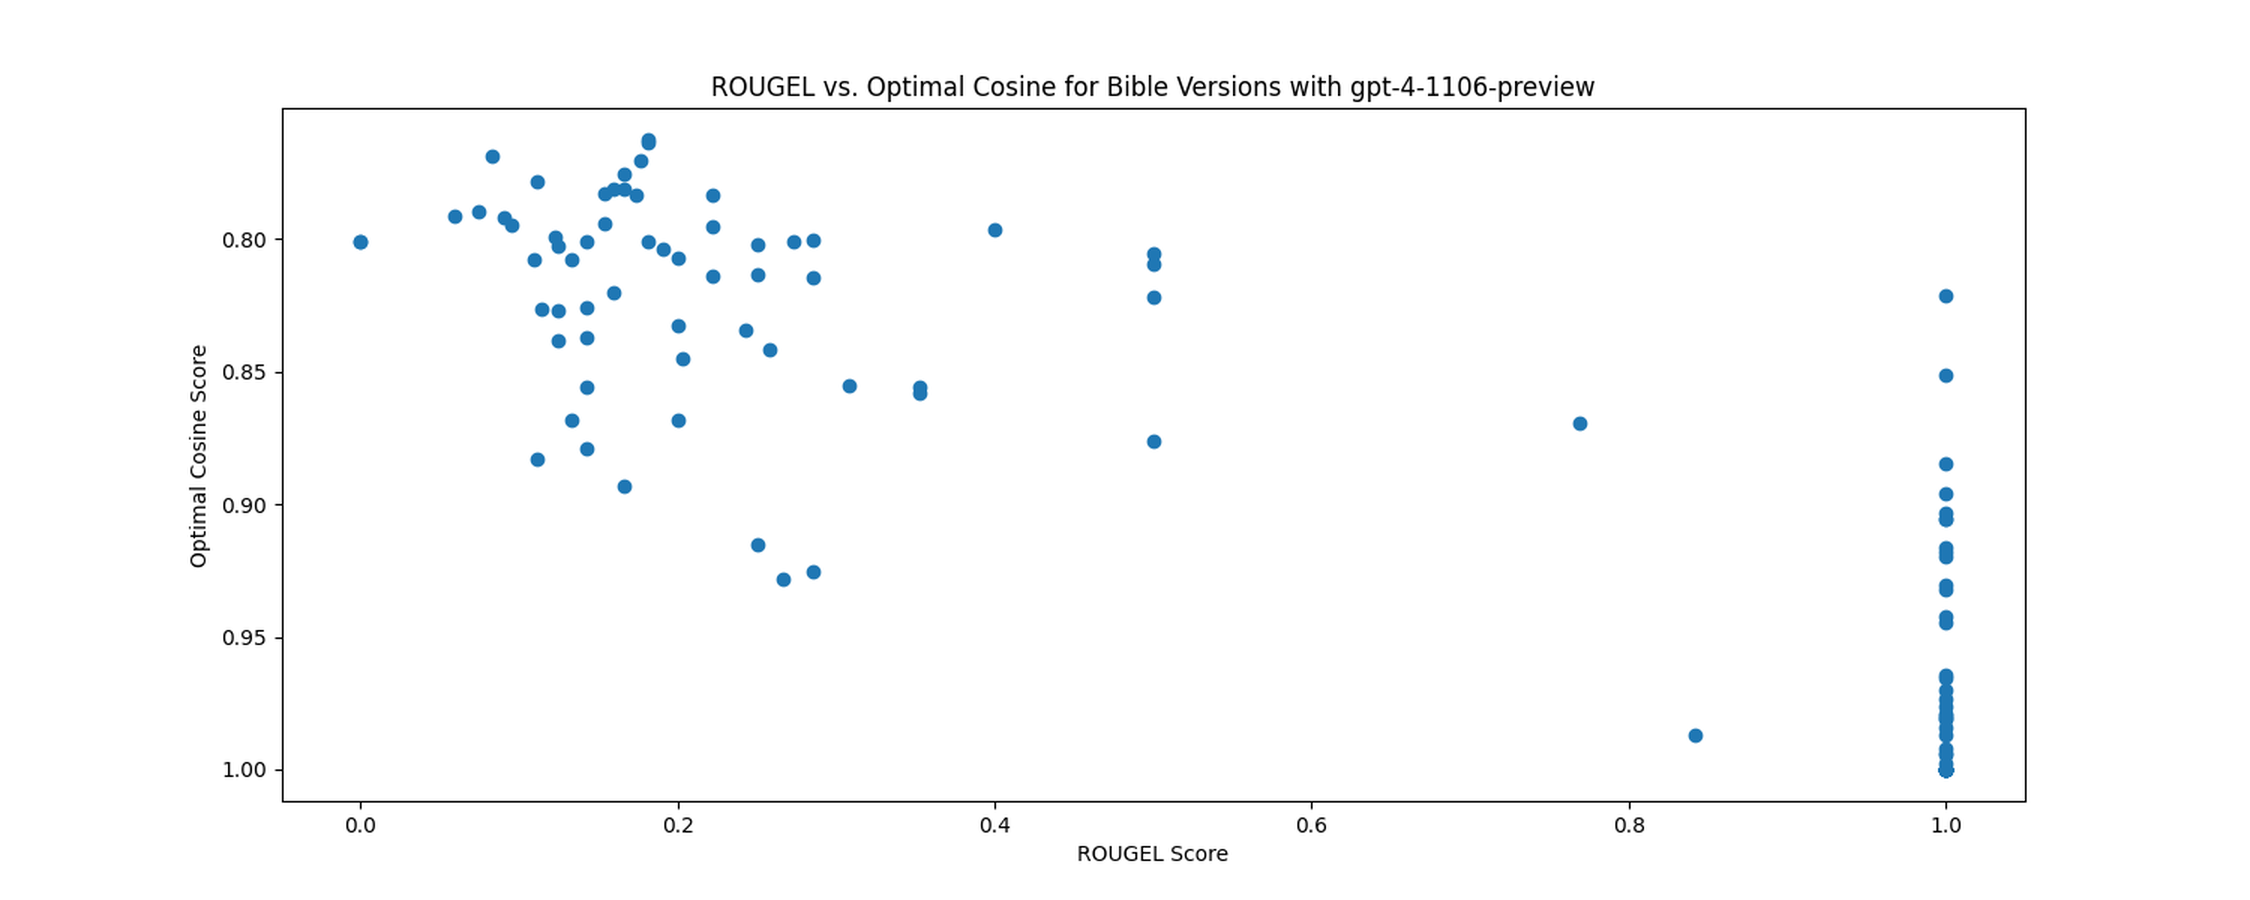
\includegraphics[width=1.0\textwidth]{bible-versions_rougeL_v_cosine-gpt-4-1106-preview.png}  \\ 
% \end{tabular} 
% \caption{RougeL vs. Cosine Similarity Score for Bible Versions} 
% \label{tab:images} 
% \end{table} 





% \begin{table}[ht] 
% \centering 
% \begin{tabular}{c} 
% 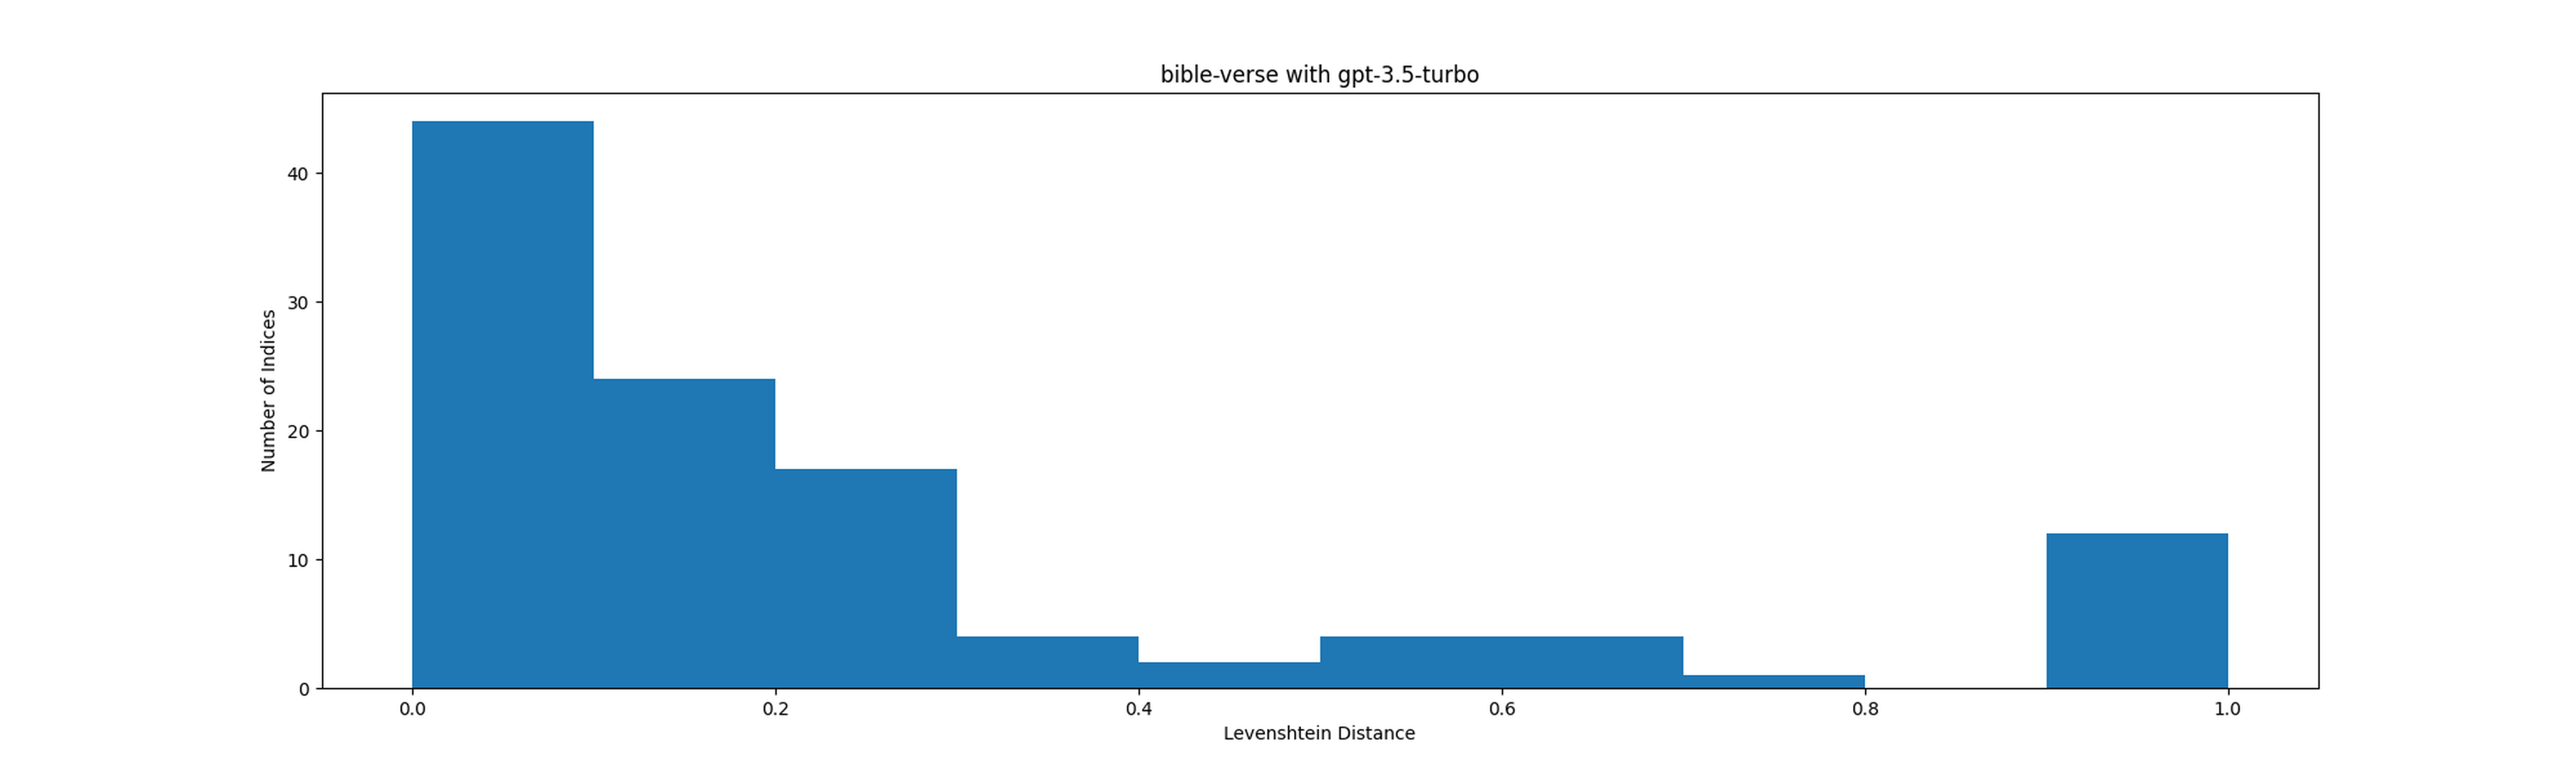
\includegraphics[width=1.0\textwidth]{bible-verse-gpt-3.5-turbo-histogram.png}  \\  
% 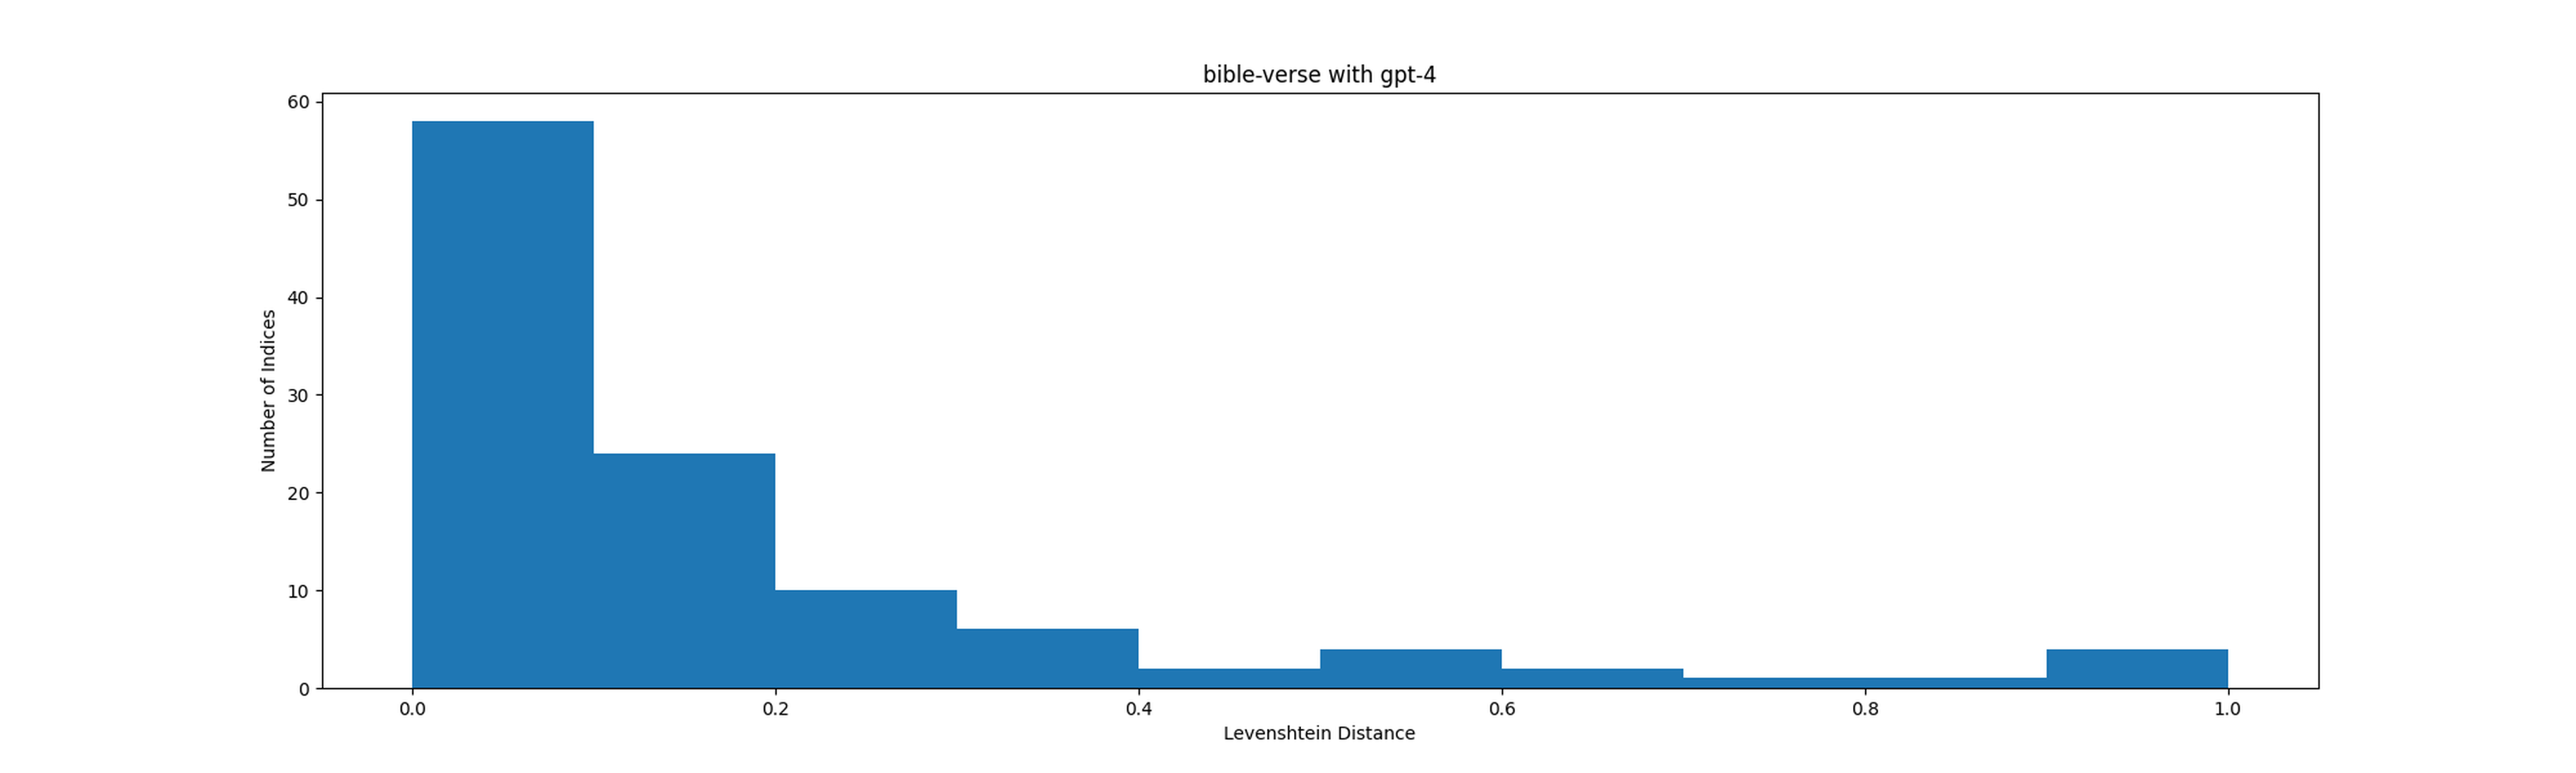
\includegraphics[width=1.0\textwidth]{bible-verse-gpt-4-histogram.png}  \\  
% 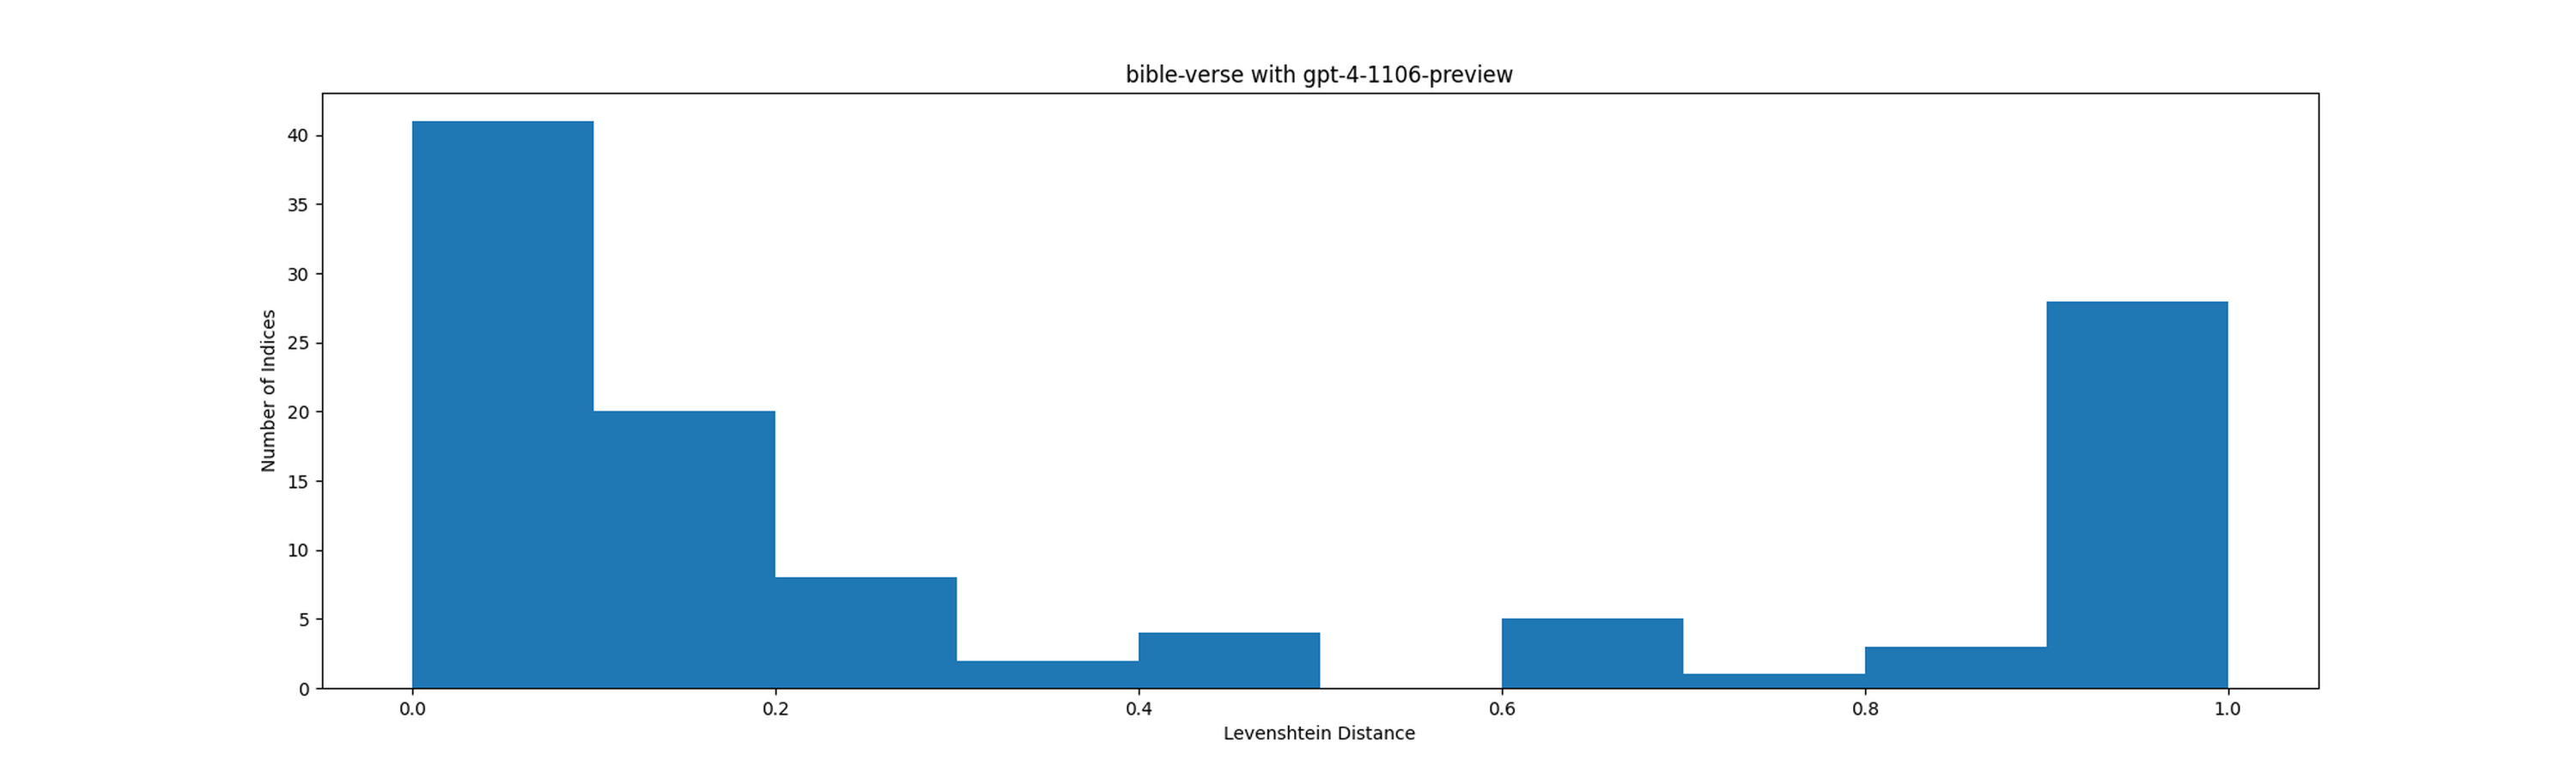
\includegraphics[width=1.0\textwidth]{bible-verse-gpt-4-1106-preview-histogram.png}  \\ 
% 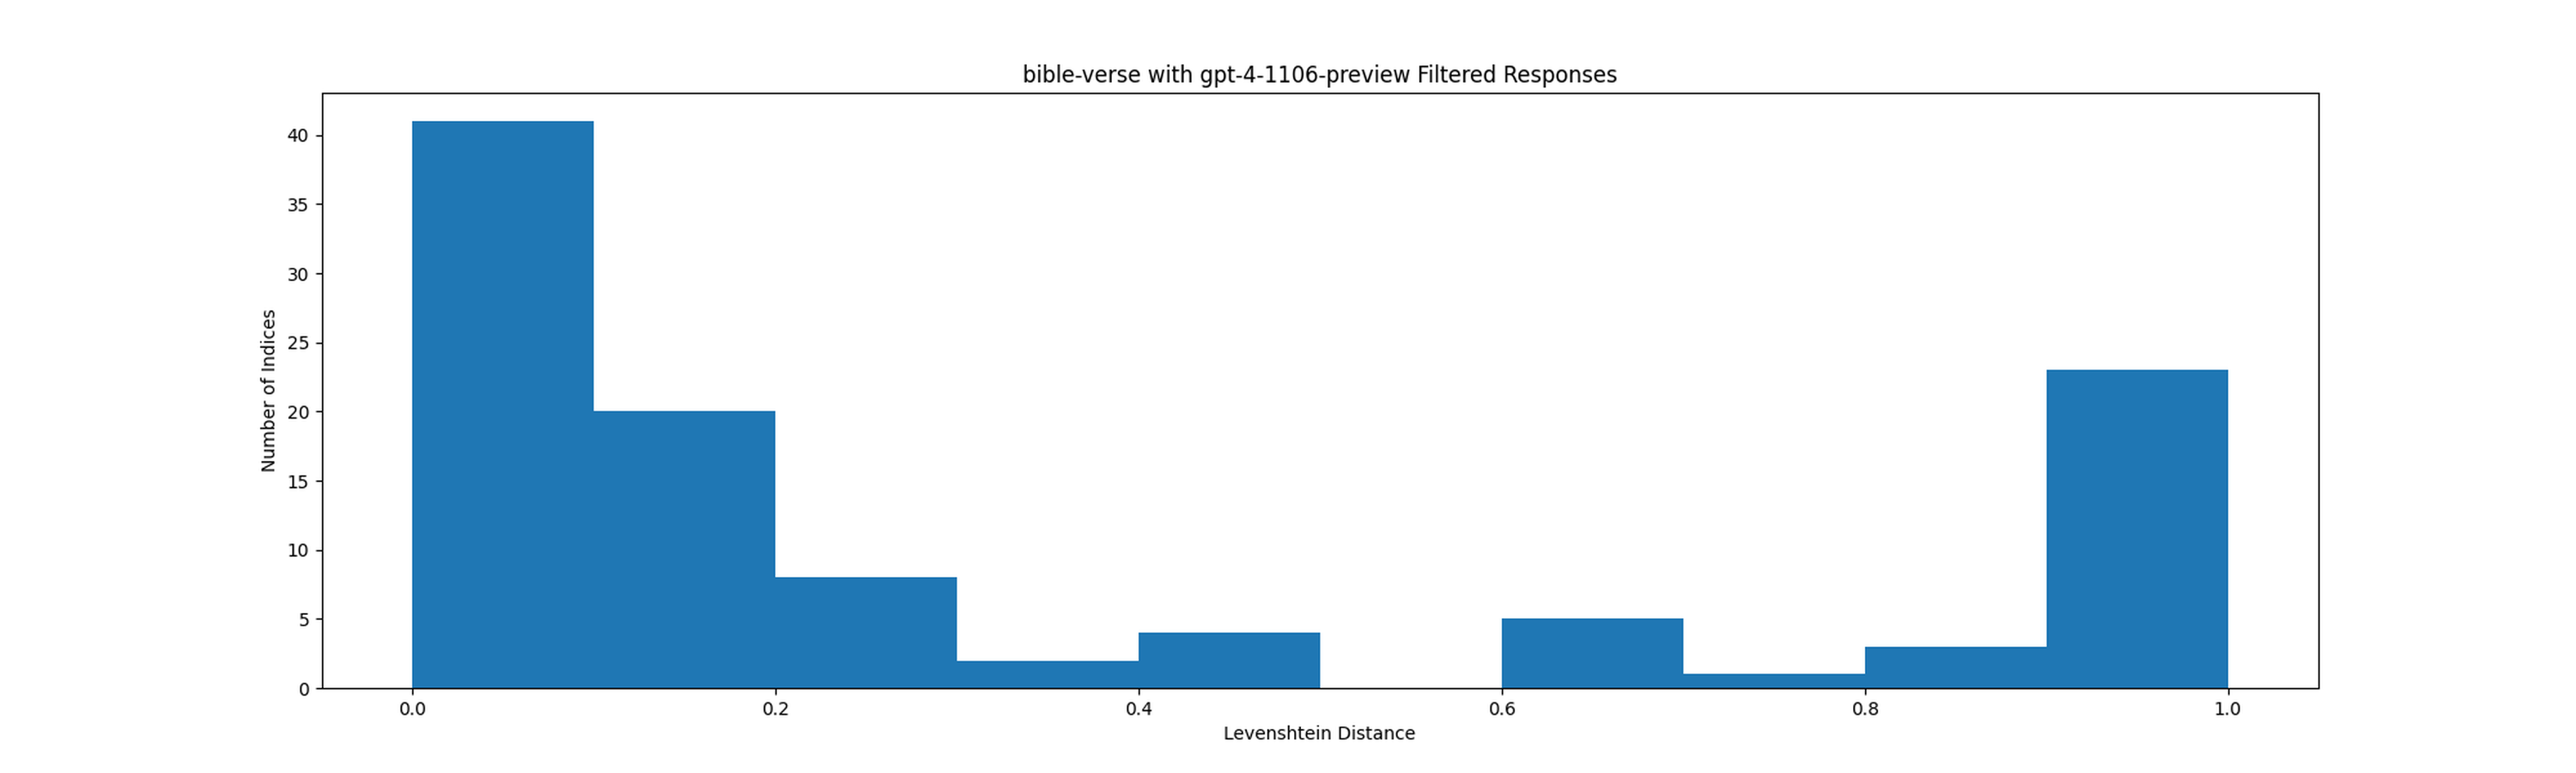
\includegraphics[width=1.0\textwidth]{bible-verse-gpt-4-1106-preview-histogram-filtered.png}  \\ 
% \end{tabular} 
% \caption{Levenshtein Distance Distribution for Bible Verses} 
% \label{tab:images} 
% \end{table} 

% \begin{table}[ht] 
% \centering 
% \begin{tabular}{c} 
% 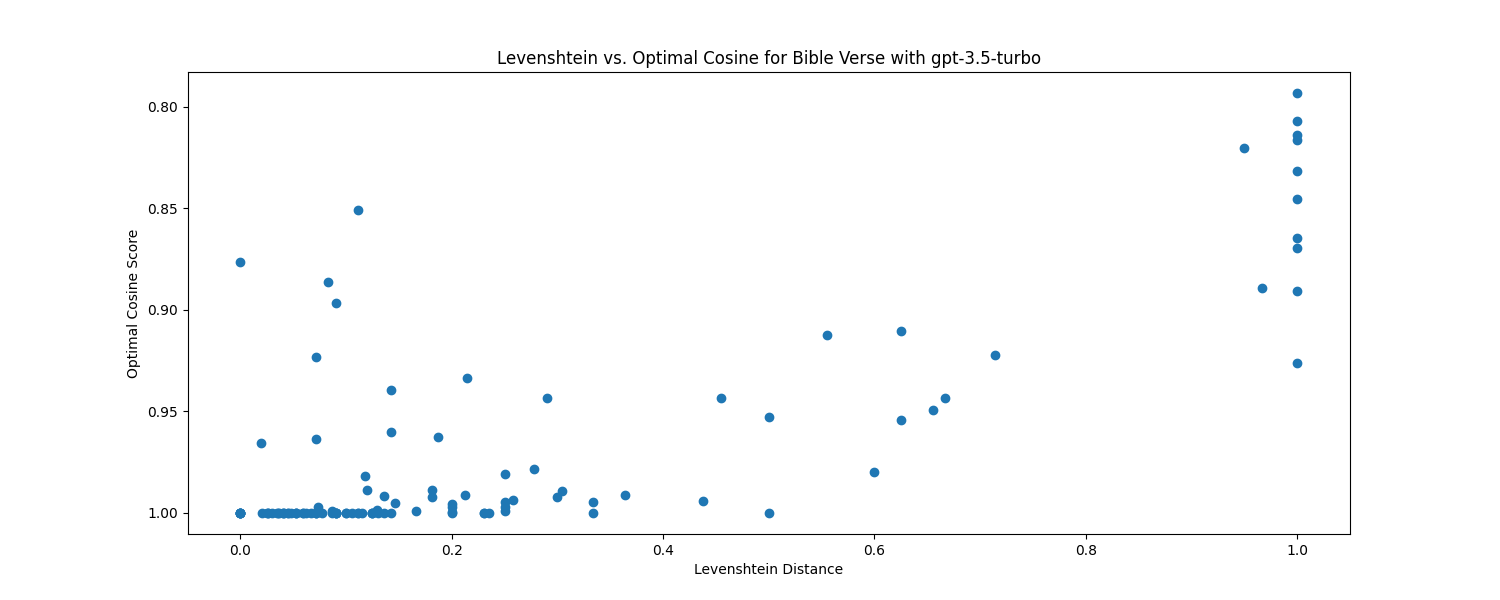
\includegraphics[width=1.0\textwidth]{bible-verse_levenshtein_v_cosine-gpt-3.5-turbo.png}  \\  
% 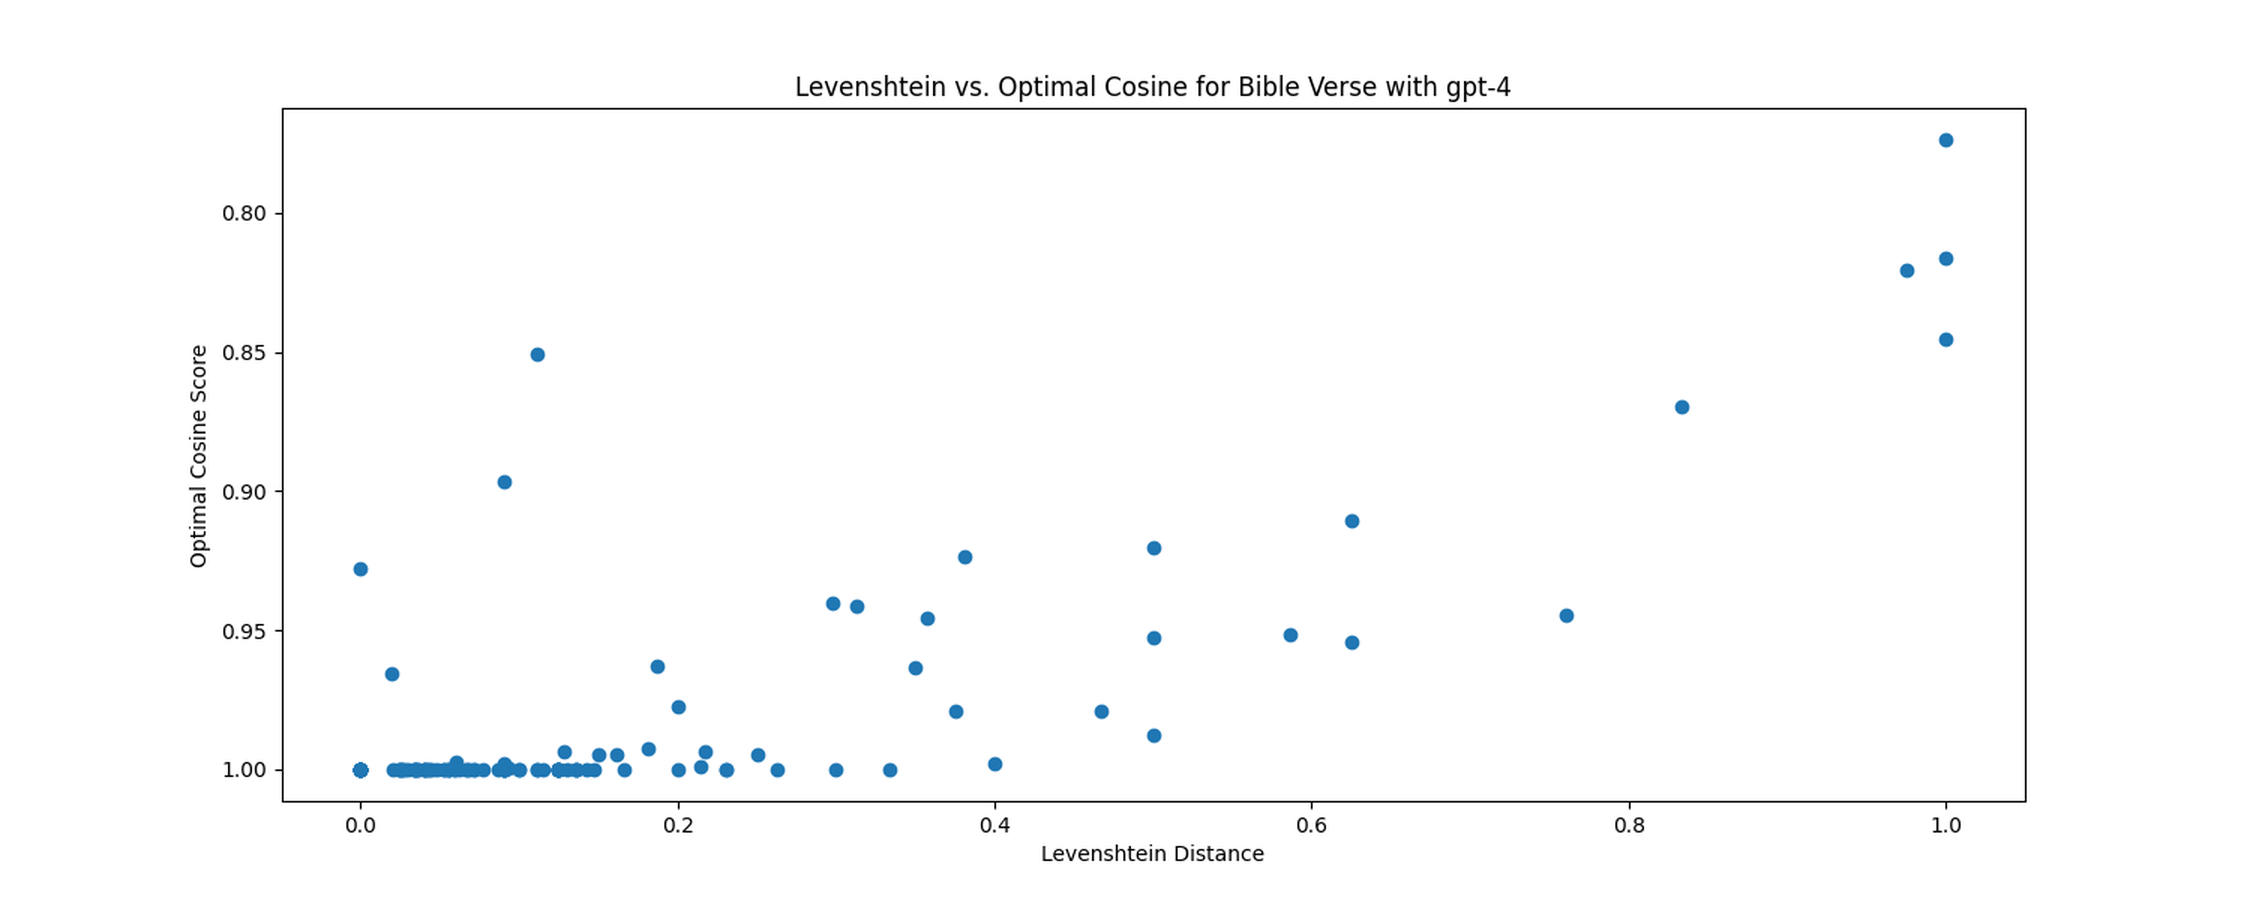
\includegraphics[width=1.0\textwidth]{bible-verse_levenshtein_v_cosine-gpt-4.png}  \\  
% \includegraphics[width=1.0\textwidth]{bible-verse_levenshtein_v_cosine-gpt-4-1106-preview.png}  \\ 
% \end{tabular} 
% \caption{Levenshtein vs. Cosine Similarity Score for Bible Verses} 
% \label{tab:images} 
% \end{table} 

% \begin{table}[ht] 
% \centering 
% \begin{tabular}{c} 
% \includegraphics[width=1.0\textwidth]{bible-verse_bleu_v_cosine-gpt-3.5-turbo.png}  \\  
% \includegraphics[width=1.0\textwidth]{bible-verse_bleu_v_cosine-gpt-4.png}  \\  
% \includegraphics[width=1.0\textwidth]{bible-verse_bleu_v_cosine-gpt-4-1106-preview.png}  \\ 
% \end{tabular} 
% \caption{Bleu vs. Cosine Similarity Score for Bible Verses} 
% \label{tab:images} 
% \end{table} 

% \begin{table}[ht] 
% \centering 
% \begin{tabular}{c} 
% \includegraphics[width=1.0\textwidth]{bible-verse_rouge1_v_cosine-gpt-3.5-turbo.png}  \\  
% \includegraphics[width=1.0\textwidth]{bible-verse_rouge1_v_cosine-gpt-4.png}  \\  
% \includegraphics[width=1.0\textwidth]{bible-verse_rouge1_v_cosine-gpt-4-1106-preview.png}  \\ 
% \end{tabular} 
% \caption{Rouge1 vs. Cosine Similarity Score for Bible Verses} 
% \label{tab:images} 
% \end{table} 

% \begin{table}[ht] 
% \centering 
% \begin{tabular}{c} 
% \includegraphics[width=1.0\textwidth]{bible-verse_rouge2_v_cosine-gpt-3.5-turbo.png}  \\  
% \includegraphics[width=1.0\textwidth]{bible-verse_rouge2_v_cosine-gpt-4.png}  \\  
% \includegraphics[width=1.0\textwidth]{bible-verse_rouge2_v_cosine-gpt-4-1106-preview.png}  \\ 
% \end{tabular} 
% \caption{Rouge2 vs. Cosine Similarity Score for Bible Verses} 
% \label{tab:images} 
% \end{table} 

% \begin{table}[ht] 
% \centering 
% \begin{tabular}{c} 
% \includegraphics[width=1.0\textwidth]{bible-verse_rougeL_v_cosine-gpt-3.5-turbo.png}  \\  
% \includegraphics[width=1.0\textwidth]{bible-verse_rougeL_v_cosine-gpt-4.png}  \\  
% \includegraphics[width=1.0\textwidth]{bible-verse_rougeL_v_cosine-gpt-4-1106-preview.png}  \\ 
% \end{tabular} 
% \caption{RougeL vs. Cosine Similarity Score for Bible Verses} 
% \label{tab:images} 
% \end{table} 


% \begin{table}[ht] 
% \centering 
% \begin{tabular}{c} 
% \includegraphics[width=1.0\textwidth]{nytimes-bestselling-romance-gpt-3.5-turbo-histogram.png}  \\  
% \includegraphics[width=1.0\textwidth]{nytimes-bestselling-romance-gpt-4-histogram.png}  \\  
% \includegraphics[width=1.0\textwidth]{nytimes-bestselling-romance-gpt-4-1106-preview-histogram.png}  \\ 
% \includegraphics[width=1.0\textwidth]{nytimes-bestselling-romance-gpt-4-1106-preview-histogram-filtered.png}  \\ 
% \end{tabular} 
% \caption{NY Times Bestselling Romance Histogram} 
% \label{tab:images} 
% \end{table} 

% \begin{table}[ht] 
% \centering 
% \begin{tabular}{c} 
% \includegraphics[width=1.0\textwidth]{nytimes-bestselling-romance_levenshtein_v_cosine-gpt-3.5-turbo.png}  \\  
% \includegraphics[width=1.0\textwidth]{nytimes-bestselling-romance_levenshtein_v_cosine-gpt-4.png}  \\  
% \includegraphics[width=1.0\textwidth]{nytimes-bestselling-romance_levenshtein_v_cosine-gpt-4-1106-preview.png}  \\ 
% \end{tabular} 
% \caption{Levenshtein vs. Cosine Similarity Score for NY Times Bestselling Romance} 
% \label{tab:images} 
% \end{table} 

% \begin{table}[ht] 
% \centering 
% \begin{tabular}{c} 
% \includegraphics[width=1.0\textwidth]{nytimes-bestselling-romance_bleu_v_cosine-gpt-3.5-turbo.png}  \\  
% \includegraphics[width=1.0\textwidth]{nytimes-bestselling-romance_bleu_v_cosine-gpt-4.png}  \\  
% \includegraphics[width=1.0\textwidth]{nytimes-bestselling-romance_bleu_v_cosine-gpt-4-1106-preview.png}  \\ 
% \end{tabular} 
% \caption{Bleu vs. Cosine Similarity Score for NY Times Bestselling Romance} 
% \label{tab:images} 
% \end{table} 

% \begin{table}[ht] 
% \centering 
% \begin{tabular}{c} 
% \includegraphics[width=1.0\textwidth]{nytimes-bestselling-romance_rouge1_v_cosine-gpt-3.5-turbo.png}  \\  
% \includegraphics[width=1.0\textwidth]{nytimes-bestselling-romance_rouge1_v_cosine-gpt-4.png}  \\  
% \includegraphics[width=1.0\textwidth]{nytimes-bestselling-romance_rouge1_v_cosine-gpt-4-1106-preview.png}  \\ 
% \end{tabular} 
% \caption{Rouge1 vs. Cosine Similarity Score for NY Times Bestselling Romance} 
% \label{tab:images} 
% \end{table} 


% \begin{table}[ht] 
% \centering 
% \begin{tabular}{c} 
% \includegraphics[width=1.0\textwidth]{nytimes-bestselling-romance_rouge2_v_cosine-gpt-3.5-turbo.png}  \\  
% \includegraphics[width=1.0\textwidth]{nytimes-bestselling-romance_rouge2_v_cosine-gpt-4.png}  \\  
% \includegraphics[width=1.0\textwidth]{nytimes-bestselling-romance_rouge2_v_cosine-gpt-4-1106-preview.png}  \\ 
% \end{tabular} 
% \caption{Rouge2 vs. Cosine Similarity Score for NY Times Bestselling Romance} 
% \label{tab:images} 
% \end{table} 

% \begin{table}[ht] 
% \centering 
% \begin{tabular}{c} 
% \includegraphics[width=1.0\textwidth]{nytimes-bestselling-romance_rougeL_v_cosine-gpt-3.5-turbo.png}  \\  
% \includegraphics[width=1.0\textwidth]{nytimes-bestselling-romance_rougeL_v_cosine-gpt-4.png}  \\  
% \includegraphics[width=1.0\textwidth]{nytimes-bestselling-romance_rougeL_v_cosine-gpt-4-1106-preview.png}  \\ 
% \end{tabular} 
% \caption{RougeL vs. Cosine Similarity Score for NY Times Bestselling Romance} 
% \label{tab:images} 
% \end{table} 

% \begin{table}[ht] 
% \centering 
% \begin{tabular}{c} 
% \includegraphics[width=1.0\textwidth]{popular-slogan-gpt-3.5-turbo-histogram.png}  \\  
% \includegraphics[width=1.0\textwidth]{popular-slogan-gpt-4-histogram.png}  \\  
% \includegraphics[width=1.0\textwidth]{popular-slogan-gpt-4-1106-preview-histogram.png}  \\ 
% \includegraphics[width=1.0\textwidth]{popular-slogan-gpt-4-1106-preview-histogram-filtered.png}  \\ 
% \end{tabular} 
% \caption{Levenshtein Distance Distribution for Popular Slogans} 
% \label{tab:images} 
% \end{table} 

% \begin{table}[ht] 
% \centering 
% \begin{tabular}{c} 
% \includegraphics[width=1.0\textwidth]{popular-slogan_levenshtein_v_cosine-gpt-3.5-turbo.png}  \\  
% \includegraphics[width=1.0\textwidth]{popular-slogan_levenshtein_v_cosine-gpt-4.png}  \\  
% \includegraphics[width=1.0\textwidth]{popular-slogan_levenshtein_v_cosine-gpt-4-1106-preview.png}  \\ 
% \end{tabular} 
% \caption{Levenshtein vs. Cosine Similarity Score for Popular Slogans} 
% \label{tab:images} 
% \end{table} 

% \begin{table}[ht] 
% \centering 
% \begin{tabular}{c} 
% \includegraphics[width=1.0\textwidth]{popular-slogan_bleu_v_cosine-gpt-3.5-turbo.png}  \\  
% \includegraphics[width=1.0\textwidth]{popular-slogan_bleu_v_cosine-gpt-4.png}  \\  
% \includegraphics[width=1.0\textwidth]{popular-slogan_bleu_v_cosine-gpt-4-1106-preview.png}  \\ 
% \end{tabular} 
% \caption{Bleu vs. Cosine Similarity Score for Popular Slogans} 
% \label{tab:images} 
% \end{table} 

% \begin{table}[ht] 
% \centering 
% \begin{tabular}{c} 
% \includegraphics[width=1.0\textwidth]{popular-slogan_rouge1_v_cosine-gpt-3.5-turbo.png}  \\  
% \includegraphics[width=1.0\textwidth]{popular-slogan_rouge1_v_cosine-gpt-4.png}  \\  
% \includegraphics[width=1.0\textwidth]{popular-slogan_rouge1_v_cosine-gpt-4-1106-preview.png}  \\ 
% \end{tabular} 
% \caption{Rouge1 vs. Cosine Similarity Score for Popular Slogans} 
% \label{tab:images} 
% \end{table} 

% \begin{table}[ht] 
% \centering 
% \begin{tabular}{c} 
% \includegraphics[width=1.0\textwidth]{popular-slogan_rouge2_v_cosine-gpt-3.5-turbo.png}  \\  
% \includegraphics[width=1.0\textwidth]{popular-slogan_rouge2_v_cosine-gpt-4.png}  \\  
% \includegraphics[width=1.0\textwidth]{popular-slogan_rouge2_v_cosine-gpt-4-1106-preview.png}  \\ 
% \end{tabular} 
% \caption{Rouge2 vs. Cosine Similarity Score for Popular Slogans} 
% \label{tab:images} 
% \end{table} 

% \begin{table}[ht] 
% \centering 
% \begin{tabular}{c} 
% \includegraphics[width=1.0\textwidth]{popular-slogan_rougeL_v_cosine-gpt-3.5-turbo.png}  \\  
% \includegraphics[width=1.0\textwidth]{popular-slogan_rougeL_v_cosine-gpt-4.png}  \\  
% \includegraphics[width=1.0\textwidth]{popular-slogan_rougeL_v_cosine-gpt-4-1106-preview.png}  \\ 
% \end{tabular} 
% \caption{RougeL vs. Cosine Similarity Score for Popular Slogans} 
% \label{tab:images} 
% \end{table} 



% \begin{table}[ht] 
% \centering 
% \begin{tabular}{c} 
% \includegraphics[width=1.0\textwidth]{famous-quote-gpt-3.5-turbo-histogram.png}  \\  
% \includegraphics[width=1.0\textwidth]{famous-quote-gpt-4-histogram.png}  \\  
% \includegraphics[width=1.0\textwidth]{famous-quote-gpt-4-1106-preview-histogram.png}  \\ 
% \includegraphics[width=1.0\textwidth]{famous-quote-gpt-4-1106-preview-histogram-filtered.png}  \\ 
% \end{tabular} 
% \caption{Levenshtein Distance Distribution for Famous Quotes} 
% \label{tab:images} 
% \end{table} 

% \begin{table}[ht] 
% \centering 
% \begin{tabular}{c} 
% \includegraphics[width=1.0\textwidth]{famous-quote_levenshtein_v_cosine-gpt-3.5-turbo.png}  \\  
% \includegraphics[width=1.0\textwidth]{famous-quote_levenshtein_v_cosine-gpt-4.png}  \\  
% \includegraphics[width=1.0\textwidth]{famous-quote_levenshtein_v_cosine-gpt-4-1106-preview.png}  \\ 
% \end{tabular} 
% \caption{Levenshtein vs. Cosine Similarity Score for Famous Quotes} 
% \label{tab:images} 
% \end{table} 

% \begin{table}[ht] 
% \centering 
% \begin{tabular}{c} 
% \includegraphics[width=1.0\textwidth]{famous-quote_bleu_v_cosine-gpt-3.5-turbo.png}  \\  
% \includegraphics[width=1.0\textwidth]{famous-quote_bleu_v_cosine-gpt-4.png}  \\  
% \includegraphics[width=1.0\textwidth]{famous-quote_bleu_v_cosine-gpt-4-1106-preview.png}  \\ 
% \end{tabular} 
% \caption{Bleu vs. Cosine Similarity Score for Famous Quotes} 
% \label{tab:images} 
% \end{table} 

% \begin{table}[ht] 
% \centering 
% \begin{tabular}{c} 
% \includegraphics[width=1.0\textwidth]{famous-quote_rouge1_v_cosine-gpt-3.5-turbo.png}  \\  
% \includegraphics[width=1.0\textwidth]{famous-quote_rouge1_v_cosine-gpt-4.png}  \\  
% \includegraphics[width=1.0\textwidth]{famous-quote_rouge1_v_cosine-gpt-4-1106-preview.png}  \\ 
% \end{tabular} 
% \caption{Rouge1 vs. Cosine Similarity Score for Famous Quotes} 
% \label{tab:images} 
% \end{table} 

% \begin{table}[ht] 
% \centering 
% \begin{tabular}{c} 
% \includegraphics[width=1.0\textwidth]{famous-quote_rouge2_v_cosine-gpt-3.5-turbo.png}  \\  
% \includegraphics[width=1.0\textwidth]{famous-quote_rouge2_v_cosine-gpt-4.png}  \\  
% \includegraphics[width=1.0\textwidth]{famous-quote_rouge2_v_cosine-gpt-4-1106-preview.png}  \\ 
% \end{tabular} 
% \caption{Rouge2 vs. Cosine Similarity Score for Famous Quotes} 
% \label{tab:images} 
% \end{table} 

% \begin{table}[ht] 
% \centering 
% \begin{tabular}{c} 
% \includegraphics[width=1.0\textwidth]{famous-quote_rougeL_v_cosine-gpt-3.5-turbo.png}  \\  
% \includegraphics[width=1.0\textwidth]{famous-quote_rougeL_v_cosine-gpt-4.png}  \\  
% \includegraphics[width=1.0\textwidth]{famous-quote_rougeL_v_cosine-gpt-4-1106-preview.png}  \\ 
% \end{tabular} 
% \caption{RougeL vs. Cosine Similarity Score for Famous Quotes} 
% \label{tab:images} 
% \end{table} 

% \begin{table}[ht] 
% \centering 
% \begin{tabular}{c}  
% \includegraphics[width=1.0\textwidth]{constitution-gpt-3.5-turbo-histogram.png}  \\  
% \includegraphics[width=1.0\textwidth]{constitution-gpt-4-histogram.png}  \\ 
% \includegraphics[width=1.0\textwidth]{constitution-gpt-4-1106-preview-histogram.png}  \\   
% \includegraphics[width=1.0\textwidth]{constitution-gpt-4-1106-preview-histogram-filtered.png}  \\  
% \end{tabular} 
% \caption{Levenshtein Distance Distribution for the Constitution} 
% \label{tab:images} 
% \end{table} 

% \begin{table}[ht] 
% \centering 
% \begin{tabular}{c}  
% \includegraphics[width=1.0\textwidth]{constitution-gpt-3.5-turbo-2d-histogram.png}  \\  
% \includegraphics[width=1.0\textwidth]{constitution-gpt-4-2d-histogram.png}  \\  
% \includegraphics[width=1.0\textwidth]{constitution-gpt-4-1106-preview-2d-histogram.png}  \\  
% \end{tabular} 
% \caption{Levenshtein Distance Distribution per Section of the Constitution} 
% \label{tab:images} 
% \end{table} 

% \begin{table}[ht] 
% \centering 
% \begin{tabular}{c}  
% \includegraphics[width=1.0\textwidth]{constitution_levenshtein_v_cosine-gpt-3.5-turbo.png}  \\  
% \includegraphics[width=1.0\textwidth]{constitution_levenshtein_v_cosine-gpt-4.png}  \\ 
% \includegraphics[width=1.0\textwidth]{constitution_levenshtein_v_cosine-gpt-4-1106-preview.png}  \\  
% \end{tabular} 
% \caption{Levenshtein Distance vs. Cosine Similarity Score for the Constitution} 
% \label{tab:images} 
% \end{table}

% \begin{table}[ht] 
% \centering 
% \begin{tabular}{c}  
% \includegraphics[width=1.0\textwidth]{constitution_bleu_v_cosine-gpt-3.5-turbo.png}  \\  
% \includegraphics[width=1.0\textwidth]{constitution_bleu_v_cosine-gpt-4.png}  \\ 
% \includegraphics[width=1.0\textwidth]{constitution_bleu_v_cosine-gpt-4-1106-preview.png}  \\  
% \end{tabular} 
% \caption{Bleu vs. Cosine Similarity Score for the Constitution} 
% \label{tab:images} 
% \end{table}

% \begin{table}[ht] 
% \centering 
% \begin{tabular}{c}  
% \includegraphics[width=1.0\textwidth]{constitution_rouge1_v_cosine-gpt-3.5-turbo.png}  \\  
% \includegraphics[width=1.0\textwidth]{constitution_rouge1_v_cosine-gpt-4.png}  \\ 
% \includegraphics[width=1.0\textwidth]{constitution_rouge1_v_cosine-gpt-4-1106-preview.png}  \\  
% \end{tabular} 
% \caption{Rouge1 vs. Cosine Similarity Score for the Constitution} 
% \label{tab:images} 
% \end{table}

% \begin{table}[ht] 
% \centering 
% \begin{tabular}{c}  
% \includegraphics[width=1.0\textwidth]{constitution_rouge2_v_cosine-gpt-3.5-turbo.png}  \\  
% \includegraphics[width=1.0\textwidth]{constitution_rouge2_v_cosine-gpt-4.png}  \\ 
% \includegraphics[width=1.0\textwidth]{constitution_rouge2_v_cosine-gpt-4-1106-preview.png}  \\  
% \end{tabular} 
% \caption{Rouge2 vs. Cosine Similarity Score for the Constitution} 
% \label{tab:images} 
% \end{table}

% \begin{table}[ht] 
% \centering 
% \begin{tabular}{c}  
% \includegraphics[width=1.0\textwidth]{constitution_rougeL_v_cosine-gpt-3.5-turbo.png}  \\  
% \includegraphics[width=1.0\textwidth]{constitution_rougeL_v_cosine-gpt-4.png}  \\ 
% \includegraphics[width=1.0\textwidth]{constitution_rougeL_v_cosine-gpt-4-1106-preview.png}  \\  
% \end{tabular} 
% \caption{RougeL vs. Cosine Similarity Score for the Constitution} 
% \label{tab:images} 
% \end{table}

% \begin{table}[ht] 
% \centering 
% \begin{tabular}{c}  
% \includegraphics[width=1.0\textwidth]{copyright-lawsuit-works-gpt-3.5-turbo-histogram.png}  \\   
% \includegraphics[width=1.0\textwidth]{copyright-lawsuit-works-gpt-4-histogram.png}  \\    
% \includegraphics[width=1.0\textwidth]{copyright-lawsuit-works-gpt-4-1106-preview-histogram.png}  \\ 
% \includegraphics[width=1.0\textwidth]{copyright-lawsuit-works-gpt-4-1106-preview-histogram-filtered.png}  \\
% \end{tabular} 
% \caption{Levenshtein Distance Distribution for Copyright Lawsuit Works} 
% \label{tab:images} 
% \end{table} 

% \begin{table}[ht] 
% \centering 
% \begin{tabular}{c}  
% \includegraphics[width=1.0\textwidth]{copyright-lawsuit-works-gpt-3.5-turbo-2d-histogram.png}  \\  
% \includegraphics[width=1.0\textwidth]{copyright-lawsuit-works-gpt-4-2d-histogram.png}  \\  
% \includegraphics[width=1.0\textwidth]{copyright-lawsuit-works-gpt-4-1106-preview-2d-histogram.png}  \\  
% \end{tabular} 
% \caption{Levenshtein Distance Distribution per Title in Copyright Lawsuit Works} 
% \label{tab:images} 
% \end{table} 

% \begin{table}[ht] 
% \centering 
% \begin{tabular}{ccc}  
% \includegraphics[width=1.0\textwidth]{copyright-lawsuit-works_levenshtein_v_cosine-gpt-3.5-turbo.png}  \\  
% \includegraphics[width=1.0\textwidth]{copyright-lawsuit-works_levenshtein_v_cosine-gpt-4.png}  \\ 
% \includegraphics[width=1.0\textwidth]{copyright-lawsuit-works_levenshtein_v_cosine-gpt-4-1106-preview.png}  \\  
% \end{tabular} 
% \caption{Levenshtein Distance vs. Cosine Similarity Score for Copyright Lawsuit Works} 
% \label{tab:images} 
% \end{table}

% \begin{table}[ht] 
% \centering 
% \begin{tabular}{c}  
% \includegraphics[width=1.0\textwidth]{copyright-lawsuit-works_bleu_v_cosine-gpt-3.5-turbo.png}  \\  
% \includegraphics[width=1.0\textwidth]{copyright-lawsuit-works_bleu_v_cosine-gpt-4.png}  \\ 
% \includegraphics[width=1.0\textwidth]{copyright-lawsuit-works_bleu_v_cosine-gpt-4-1106-preview.png}  \\  
% \end{tabular} 
% \caption{Bleu vs. Cosine Similarity Score for Copyright Lawsuit Works} 
% \label{tab:images} 
% \end{table}

% \begin{table}[ht] 
% \centering 
% \begin{tabular}{c}  
% \includegraphics[width=1.0\textwidth]{copyright-lawsuit-works_rouge1_v_cosine-gpt-3.5-turbo.png}  \\  
% \includegraphics[width=1.0\textwidth]{copyright-lawsuit-works_rouge1_v_cosine-gpt-4.png}  \\ 
% \includegraphics[width=1.0\textwidth]{copyright-lawsuit-works_rouge1_v_cosine-gpt-4-1106-preview.png}  \\  
% \end{tabular} 
% \caption{Rouge1 vs. Cosine Similarity Score for Copyright Lawsuit Works} 
% \label{tab:images} 
% \end{table}

% \begin{table}[ht] 
% \centering 
% \begin{tabular}{c}  
% \includegraphics[width=1.0\textwidth]{copyright-lawsuit-works_rouge2_v_cosine-gpt-3.5-turbo.png}  \\  
% \includegraphics[width=1.0\textwidth]{copyright-lawsuit-works_rouge2_v_cosine-gpt-4.png}  \\ 
% \includegraphics[width=1.0\textwidth]{copyright-lawsuit-works_rouge2_v_cosine-gpt-4-1106-preview.png}  \\  
% \end{tabular} 
% \caption{Rouge2 vs. Cosine Similarity Score for Copyright Lawsuit Works} 
% \label{tab:images} 
% \end{table}

% \begin{table}[ht] 
% \centering 
% \begin{tabular}{c}  
% \includegraphics[width=1.0\textwidth]{copyright-lawsuit-works_rougeL_v_cosine-gpt-3.5-turbo.png}  \\  
% \includegraphics[width=1.0\textwidth]{copyright-lawsuit-works_rougeL_v_cosine-gpt-4.png}  \\ 
% \includegraphics[width=1.0\textwidth]{copyright-lawsuit-works_rougeL_v_cosine-gpt-4-1106-preview.png}  \\  
% \end{tabular} 
% \caption{RougeL vs. Cosine Similarity Score for Copyright Lawsuit Works} 
% \label{tab:images} 
% \end{table}

% \begin{table}[ht] 
% \centering 
% \begin{tabular}{c}  
% \includegraphics[width=1.0\textwidth]{fantasy-gpt-3.5-turbo-histogram.png}  \\   
% \includegraphics[width=1.0\textwidth]{fantasy-gpt-4-histogram-filtered.png}  \\    
% \includegraphics[width=1.0\textwidth]{fantasy-gpt-4-1106-preview-histogram-filtered.png}  \\ 
% \includegraphics[width=1.0\textwidth]{fantasy-gpt-4-1106-preview-histogram.png}  \\
% \end{tabular} 
% \caption{Levenshtein Distance Distribution for Fantasy Works} 
% \label{tab:images} 
% \end{table} 


% \begin{table}[ht] 
% \centering 
% \begin{tabular}{c} 
% \includegraphics[width=1.0\textwidth]{fantasy_bleu_v_cosine-gpt-3.5-turbo.png}  \\  
% \includegraphics[width=1.0\textwidth]{fantasy_bleu_v_cosine-gpt-4.png}  \\  
% \includegraphics[width=1.0\textwidth]{fantasy_bleu_v_cosine-gpt-4-1106-preview.png}  \\ 
% \end{tabular} 
% \caption{Fantasy Bleu vs Cosine Scatterplots} 
% \label{tab:images} 
% \end{table} 

% \begin{table}[ht] 
% \centering 
% \begin{tabular}{c} 
% \includegraphics[width=1.0\textwidth]{fantasy_rouge1_v_cosine-gpt-3.5-turbo.png}  \\  
% \includegraphics[width=1.0\textwidth]{fantasy_rouge1_v_cosine-gpt-4.png}  \\  
% \includegraphics[width=1.0\textwidth]{fantasy_rouge1_v_cosine-gpt-4-1106-preview.png}  \\ 
% \end{tabular} 
% \caption{Fantasy Rouge1 vs Cosine Scatterplots} 
% \label{tab:images} 
% \end{table} 

% \begin{table}[ht] 
% \centering 
% \begin{tabular}{c} 
% \includegraphics[width=1.0\textwidth]{fantasy_rouge2_v_cosine-gpt-3.5-turbo.png}  \\  
% \includegraphics[width=1.0\textwidth]{fantasy_rouge2_v_cosine-gpt-4.png}  \\  
% \includegraphics[width=1.0\textwidth]{fantasy_rouge2_v_cosine-gpt-4-1106-preview.png}  \\ 
% \end{tabular} 
% \caption{Fantasy Rouge2 vs Cosine Scatterplots} 
% \label{tab:images} 
% \end{table} 

% \begin{table}[ht] 
% \centering 
% \begin{tabular}{c} 
% \includegraphics[width=1.0\textwidth]{fantasy_rougeL_v_cosine-gpt-3.5-turbo.png}  \\  
% \includegraphics[width=1.0\textwidth]{fantasy_rougeL_v_cosine-gpt-4-1106-preview.png}  \\  
% \includegraphics[width=1.0\textwidth]{fantasy_rougeL_v_cosine-gpt-4-1106-preview.png}  \\ 
% \end{tabular} 
% \caption{Fantasy RougeL vs Cosine Scatterplots} 
% \label{tab:images} 
% \end{table} 



% \begin{table}[ht] 
% \centering 
% \begin{tabular}{c}  
% \includegraphics[width=1.0\textwidth]{fantasy-gpt-3.5-turbo-2d-histogram.png}  \\  
% \includegraphics[width=1.0\textwidth]{fantasy-gpt-4-2d-histogram.png}  \\  
% \includegraphics[width=1.0\textwidth]{fantasy-gpt-4-1106-preview-2d-histogram.png}  \\  
% \end{tabular} 
% \caption{Levenshtein Distance Distribution per Title in Fantasy Works}
% \label{tab:images} 
% \end{table} 

% \begin{table}[ht] 
% \centering 
% \begin{tabular}{c}  
% \includegraphics[width=1.0\textwidth]{fantasy_levenshtein_v_cosine-gpt-3.5-turbo.png}  \\  
% \includegraphics[width=1.0\textwidth]{fantasy_levenshtein_v_cosine-gpt-4.png}  \\ 
% \includegraphics[width=1.0\textwidth]{fantasy_levenshtein_v_cosine-gpt-4-1106-preview.png}  \\  
% \end{tabular} 
% \caption{Levenshtein Distance vs. Cosine Similarity Score for Fantasy Works} 
% \label{tab:images} 
% \end{table}

% \begin{table}[ht] 
% \centering 
% \begin{tabular}{c}  
% \includegraphics[width=1.0\textwidth]{published-post-model-gpt-3.5-turbo-histogram.png}  \\   
% \includegraphics[width=1.0\textwidth]{published-post-model-gpt-4-histogram.png}  \\    
% \includegraphics[width=1.0\textwidth]{published-post-model-gpt-4-1106-preview-histogram.png}  \\ 
% \includegraphics[width=1.0\textwidth]{published-post-model-gpt-4-1106-preview-histogram-filtered.png}  \\
% \end{tabular} 


% \caption{Levenshtein Distance Distribution for Works Published Post-GPT4} 
% \label{tab:images} 
% \end{table} 

% \begin{table}[ht] 
% \centering 
% \begin{tabular}{c}  
% \includegraphics[width=1.0\textwidth]{published-post-model-gpt-3.5-turbo-2d-histogram.png}  \\  
% \includegraphics[width=1.0\textwidth]{published-post-model-gpt-4-2d-histogram.png}  \\  
% \includegraphics[width=1.0\textwidth]{published-post-model-gpt-4-1106-preview-2d-histogram.png}  \\  
% \end{tabular} 
% \caption{Levenshtein Distance Distribution per Title in Works Published Post-GPT4}
% \label{tab:images} 
% \end{table} 

% \begin{table}[ht] 
% \centering 
% \begin{tabular}{c}  
% \includegraphics[width=1.0\textwidth]{published-post-model_levenshtein_v_cosine-gpt-3.5-turbo.png}  \\  
% \includegraphics[width=1.0\textwidth]{published-post-model_levenshtein_v_cosine-gpt-4.png}  \\ 
% \includegraphics[width=1.0\textwidth]{published-post-model_levenshtein_v_cosine-gpt-4-1106-preview.png}  \\  
% \end{tabular} 
% \caption{Levenshtein Distance vs. Cosine Similarity Score for Works Published Post-GPT4} 
% \label{tab:images} 
% \end{table}

% \begin{table}[ht] 
% \centering 
% \begin{tabular}{c}  
% \includegraphics[width=1.0\textwidth]{published-post-model_bleu_v_cosine-gpt-3.5-turbo.png}  \\  
% \includegraphics[width=1.0\textwidth]{published-post-model_bleu_v_cosine-gpt-4.png}  \\ 
% \includegraphics[width=1.0\textwidth]{published-post-model_bleu_v_cosine-gpt-4-1106-preview.png}  \\  
% \end{tabular} 
% \caption{BLEU Distance vs. Cosine Similarity Score for Works Published Post-GPT4} 
% \label{tab:images} 
% \end{table}

% \begin{table}[ht] 
% \centering 
% \begin{tabular}{c}  
% \includegraphics[width=1.0\textwidth]{published-post-model_rouge1_v_cosine-gpt-3.5-turbo.png}  \\  
% \includegraphics[width=1.0\textwidth]{published-post-model_rouge1_v_cosine-gpt-4.png}  \\ 
% \includegraphics[width=1.0\textwidth]{published-post-model_rouge1_v_cosine-gpt-4-1106-preview.png}  \\  
% \end{tabular} 
% \caption{Rouge1 vs. Cosine Similarity Score for Works Published Post-GPT4} 
% \label{tab:images} 
% \end{table}

% \begin{table}[ht] 
% \centering 
% \begin{tabular}{c}  
% \includegraphics[width=1.0\textwidth]{published-post-model_rouge2_v_cosine-gpt-3.5-turbo.png}  \\  
% \includegraphics[width=1.0\textwidth]{published-post-model_rouge2_v_cosine-gpt-4.png}  \\ 
% \includegraphics[width=1.0\textwidth]{published-post-model_rouge2_v_cosine-gpt-4-1106-preview.png}  \\  
% \end{tabular} 
% \caption{Rouge2 vs. Cosine Similarity Score for Works Published Post-GPT4} 
% \label{tab:images} 
% \end{table}

% \begin{table}[ht] 
% \centering 
% \begin{tabular}{c}  
% \includegraphics[width=1.0\textwidth]{published-post-model_rougeL_v_cosine-gpt-3.5-turbo.png}  \\  
% \includegraphics[width=1.0\textwidth]{published-post-model_rougeL_v_cosine-gpt-4.png}  \\ 
% \includegraphics[width=1.0\textwidth]{published-post-model_rougeL_v_cosine-gpt-4-1106-preview.png}  \\  
% \end{tabular} 
% \caption{RougeL vs. Cosine Similarity Score for Works Published Post-GPT4} 
% \label{tab:images} 
% \end{table}

% \begin{table}[ht] 
% \centering 
% \begin{tabular}{c}  
% \includegraphics[width=1.0\textwidth]{random-text-gpt-3.5-turbo-histogram.png}  \\   
% \includegraphics[width=1.0\textwidth]{random-text-gpt-3.5-turbo-histogram-filtered.png}  \\    
% \includegraphics[width=1.0\textwidth]{random-text-gpt-4-histogram.png}  \\ 
% \includegraphics[width=1.0\textwidth]{random-text-gpt-4-1106-preview-histogram.png}  \\ 
% \includegraphics[width=1.0\textwidth]{random-text-gpt-4-1106-preview-histogram-filtered.png}  \\
% \end{tabular} 
% \caption{Levenshtein Distance Distribution for Random Text Excerpts} 
% \label{tab:images} 
% \end{table} 

% \begin{table}[ht] 
% \centering
% \begin{tabular}{c}  
% \includegraphics[width=1.0\textwidth]{random-text_levenshtein_v_cosine-gpt-3.5-turbo.png}  \\  
% \includegraphics[width=1.0\textwidth]{random-text_levenshtein_v_cosine-gpt-4.png}  \\ 
% \includegraphics[width=1.0\textwidth]{random-text_levenshtein_v_cosine-gpt-4-1106-preview.png}  \\  
% \end{tabular} 
% \caption{Levenshtein Distance vs. Cosine Similarity Score for Random Text Excerpts} 
% \label{tab:images} 
% \end{table}

% \begin{table}[ht] 
% \centering 
% \begin{tabular}{c}  
% \includegraphics[width=1.0\textwidth]{random-text_bleu_v_cosine-gpt-3.5-turbo.png}  \\  
% \includegraphics[width=1.0\textwidth]{random-text_bleu_v_cosine-gpt-4.png}  \\ 
% \includegraphics[width=1.0\textwidth]{random-text_bleu_v_cosine-gpt-4-1106-preview.png}  \\  
% \end{tabular} 
% \caption{Bleu Distance vs. Cosine Similarity Score for Random Text Excerpts} 
% \label{tab:images} 
% \end{table}

% \begin{table}[ht] 
% \centering 
% \begin{tabular}{c}  
% \includegraphics[width=1.0\textwidth]{random-text_rouge1_v_cosine-gpt-3.5-turbo.png}  \\  
% \includegraphics[width=1.0\textwidth]{random-text_rouge1_v_cosine-gpt-4.png}  \\ 
% \includegraphics[width=1.0\textwidth]{random-text_rouge1_v_cosine-gpt-4-1106-preview.png}  \\  
% \end{tabular} 
% \caption{Rouge1 Distance vs. Cosine Similarity Score for Random Text Excerpts} 
% \label{tab:images} 
% \end{table}

% \begin{table}[ht] 
% \centering 
% \begin{tabular}{c}  
% \includegraphics[width=1.0\textwidth]{random-text_rouge2_v_cosine-gpt-3.5-turbo.png}  \\  
% \includegraphics[width=1.0\textwidth]{random-text_rouge2_v_cosine-gpt-4.png}  \\ 
% \includegraphics[width=1.0\textwidth]{random-text_rouge2_v_cosine-gpt-4-1106-preview.png}  \\  
% \end{tabular} 
% \caption{Rouge2 Distance vs. Cosine Similarity Score for Random Text Excerpts} 
% \label{tab:images} 
% \end{table}

% \begin{table}[ht] 
% \centering 
% \begin{tabular}{c}  
% \includegraphics[width=1.0\textwidth]{random-text_rougeL_v_cosine-gpt-3.5-turbo.png}  \\  
% \includegraphics[width=1.0\textwidth]{random-text_rougeL_v_cosine-gpt-4.png}  \\ 
% \includegraphics[width=1.0\textwidth]{random-text_rougeL_v_cosine-gpt-4-1106-preview.png}  \\  
% \end{tabular} 
% \caption{RougeL Distance vs. Cosine Similarity Score for Random Text Excerpts} 
% \label{tab:images} 
% \end{table}

% \begin{table}[ht] 
% \centering 
% \begin{tabular}{c}  
% \includegraphics[width=1.0\textwidth]{standard-lorem-ipsum-passage-gpt-3.5-turbo-histogram.png}  \\   
% \includegraphics[width=1.0\textwidth]{standard-lorem-ipsum-passage-gpt-4-histogram.png}  \\ 
% \includegraphics[width=1.0\textwidth]{standard-lorem-ipsum-passage-gpt-4-1106-preview-histogram.png}  \\    
% \includegraphics[width=1.0\textwidth]{standard-lorem-ipsum-passage-gpt-4-1106-preview-histogram-filtered.png}  \\ 
% \end{tabular} 
% \caption{Levenshtein Distance Distribution for the Standard Lorem Ipsum Passage} 
% \label{tab:images} 
% \end{table} 

% \begin{table}[ht] 
% \centering 
% \begin{tabular}{c}  
% \includegraphics[width=1.0\textwidth]{standard-lorem-ipsum-passage_levenshtein_v_cosine-gpt-3.5-turbo.png}  \\  
% \includegraphics[width=1.0\textwidth]{standard-lorem-ipsum-passage_levenshtein_v_cosine-gpt-4.png}  \\ 
% \includegraphics[width=1.0\textwidth]{standard-lorem-ipsum-passage_levenshtein_v_cosine-gpt-4-1106-preview.png}  \\  
% \end{tabular} 
% \caption{Levenshtein Distance vs. Cosine Similarity Score for the Standard Lorem Ipsum Passage} 
% \label{tab:images} 
% \end{table}

% \begin{table}[ht] 
% \centering 
% \begin{tabular}{c}  
% \includegraphics[width=1.0\textwidth]{standard-lorem-ipsum-passage_bleu_v_cosine-gpt-3.5-turbo.png}  \\  
% \includegraphics[width=1.0\textwidth]{standard-lorem-ipsum-passage_bleu_v_cosine-gpt-4.png}  \\ 
% \includegraphics[width=1.0\textwidth]{standard-lorem-ipsum-passage_bleu_v_cosine-gpt-4-1106-preview.png}  \\  
% \end{tabular} 
% \caption{BLEU vs. Cosine Similarity Score for the Standard Lorem Ipsum Passage} 
% \label{tab:images} 
% \end{table}

% \begin{table}[ht] 
% \centering 
% \begin{tabular}{c}  
% \includegraphics[width=1.0\textwidth]{standard-lorem-ipsum-passage_rouge1_v_cosine-gpt-3.5-turbo.png}  \\  
% \includegraphics[width=1.0\textwidth]{standard-lorem-ipsum-passage_rouge1_v_cosine-gpt-4.png}  \\ 
% \includegraphics[width=1.0\textwidth]{standard-lorem-ipsum-passage_rouge1_v_cosine-gpt-4-1106-preview.png}  \\  
% \end{tabular} 
% \caption{Rouge1 vs. Cosine Similarity Score for the Standard Lorem Ipsum Passage} 
% \label{tab:images} 
% \end{table}

% \begin{table}[ht] 
% \centering 
% \begin{tabular}{c}  
% \includegraphics[width=1.0\textwidth]{standard-lorem-ipsum-passage_rouge2_v_cosine-gpt-3.5-turbo.png}  \\  
% \includegraphics[width=1.0\textwidth]{standard-lorem-ipsum-passage_rouge2_v_cosine-gpt-4.png}  \\ 
% \includegraphics[width=1.0\textwidth]{standard-lorem-ipsum-passage_rouge2_v_cosine-gpt-4-1106-preview.png}  \\  
% \end{tabular} 
% \caption{Rouge2 vs. Cosine Similarity Score for the Standard Lorem Ipsum Passage} 
% \label{tab:images} 
% \end{table}

% \begin{table}[ht] 
% \centering 
% \begin{tabular}{c}  
% \includegraphics[width=1.0\textwidth]{standard-lorem-ipsum-passage_rougeL_v_cosine-gpt-3.5-turbo.png}  \\  
% \includegraphics[width=1.0\textwidth]{standard-lorem-ipsum-passage_rougeL_v_cosine-gpt-4.png}  \\ 
% \includegraphics[width=1.0\textwidth]{standard-lorem-ipsum-passage_rougeL_v_cosine-gpt-4-1106-preview.png}  \\  
% \end{tabular} 
% \caption{RougeL vs. Cosine Similarity Score for the Standard Lorem Ipsum Passage} 
% \label{tab:images} 
% \end{table}

\begin{table}[ht] 
\centering 
\begin{tabular}{c} 
\includegraphics[width=1.0\textwidth]{plots/categories-2d-histogram-gpt-3.5-turbo.png}  \\  
\includegraphics[width=1.0\textwidth]{plots/categories-2d-histogram-gpt-4.png}  \\ 
\includegraphics[width=1.0\textwidth]{plots/categories-2d-histogram-gpt-4-1106-preview.png}  \\ 
\end{tabular} 
\caption{Levenshtein Distance Distributions per Category} 
\label{tab:images} 
\end{table} 

\begin{table}[ht] 
\centering 
\begin{tabular}{c} 
\includegraphics[width=1.0\textwidth]{plots/cosine-ecdf-plot-gpt-3.5-turbo.png}  \\  
\includegraphics[width=1.0\textwidth]{plots/cosine-ecdf-plot-gpt-4.png}  \\ 
\includegraphics[width=1.0\textwidth]{plots/cosine-ecdf-plot-gpt-4-1106-preview.png}  \\ 
\end{tabular} 
\caption{Cosine Similarity ECDF Plot for All Categories} 
\label{tab:images} 
\end{table} 

% \begin{table}[ht] 
% \centering 
% \begin{tabular}{c} 
% \includegraphics[width=1.0\textwidth]{bleu-ecdf-plot-gpt-3.5-turbo.png}  \\  
% \includegraphics[width=1.0\textwidth]{bleu-ecdf-plot-gpt-4.png}  \\ 
% \includegraphics[width=1.0\textwidth]{bleu-ecdf-plot-gpt-4-1106-preview.png}  \\ 
% \end{tabular} 
% \caption{BLEU Similarity ECDF Plot for All Categories} 
% \label{tab:images} 
% \end{table}

\begin{table}[ht] 
\centering 
\begin{tabular}{c} 
\includegraphics[width=1.0\textwidth]{plots/rouge1-ecdf-plot-gpt-3.5-turbo.png}  \\  
\includegraphics[width=1.0\textwidth]{plots/rouge1-ecdf-plot-gpt-4.png}  \\ 
\includegraphics[width=1.0\textwidth]{plots/rouge1-ecdf-plot-gpt-4-1106-preview.png}  \\ 
\end{tabular} 
\caption{Rouge1 Similarity ECDF Plot for All Categories} 
\label{tab:images} 
\end{table}

\begin{table}[ht] 
\centering 
\begin{tabular}{c} 
\includegraphics[width=1.0\textwidth]{plots/rouge2-ecdf-plot-gpt-3.5-turbo.png}  \\  
\includegraphics[width=1.0\textwidth]{plots/rouge2-ecdf-plot-gpt-4.png}  \\ 
\includegraphics[width=1.0\textwidth]{plots/rouge2-ecdf-plot-gpt-4-1106-preview.png}  \\ 
\end{tabular} 
\caption{Rouge2 Similarity ECDF Plot for All Categories} 
\label{tab:images} 
\end{table}

\begin{table}[ht] 
\centering 
\begin{tabular}{c} 
\includegraphics[width=1.0\textwidth]{plots/rougeL-ecdf-plot-gpt-3.5-turbo.png}  \\  
\includegraphics[width=1.0\textwidth]{plots/rougeL-ecdf-plot-gpt-4.png}  \\ 
\includegraphics[width=1.0\textwidth]{plots/rougeL-ecdf-plot-gpt-4-1106-preview.png}  \\ 
\end{tabular} 
\caption{RougeL Similarity ECDF Plot for All Categories} 
\label{tab:images} 
\end{table}


\end{document}
